\documentclass[a4paper,11pt]{book}
\textheight 23 cm
%HEVEA\@def@charset{US-ASCII}
\usepackage[utf8]{inputenc}
\usepackage[T1]{fontenc}
\usepackage[francais]{babel}
\usepackage{latexsym}
\usepackage{amsfonts}
\usepackage{amssymb}
\usepackage{makeidx}
\usepackage{times}
%\usepackage{graphics}
\usepackage{ifpdf}
\ifpdf
 \usepackage[pdftex,colorlinks]{hyperref}
\else
 %\usepackage[ps2pdf,breaklinks=true,colorlinks=true,linkcolor=red,citecolor=green]{hyperref}
 \usepackage{pst-plot}
\fi
\usepackage{pst-plot}
\usepackage{graphicx}
\title{La tortue et la g\'eom\'etrie avec {\tt Xcas}}
\makeindex
\author{Ren\'ee De Graeve}

\begin{document}
\maketitle
\chapter*{Introduction}
La partie {\tt Tortue} de {\tt Xcas} contient des commandes permettant de faire
des dessins comme en {\tt Logo} en donnant des ordres \`a une tortue
 poss\'edant un crayon.\\
Ces dessins sont faits dans l'\'ecran graphique {\tt Tortue} qui est
obtenu avec le raccourci clavier : {\tt Alt+d}.\\

La tortue est un curseur graphique repr\'esent\'e par un triangle : 
c'est un robot orient\'e qui peut avancer, reculer, tourner sur place \`a 
droite ou \`a gauche et tracer ses d\'eplacements.\\
Contrairement \`a {\tt Logo} il n'y a pas de commandes g\'erant des changements
d'\'echelles mais il y a la possibilit\'e de d\'eplacer l'\'ecran du dessin 
avec la souris (par exemple, pour centrer le dessin) et aussi de r\'eduire 
ou d'augmenter la taille du dessin en agissant sur la molette de la souris.\\
Par rapport \`a Logo, on a ajout\'e :
\begin{itemize}
\item les commandes :
\begin{itemize}
\item{\tt saute} qui fait faire \`a la tortue des bonds en avant ou en arri\`ere et
\item {\tt pas\_de\_cote} qui fait faire \`a la 
tortue des bonds sur le c\^ot\'e  \`a gauche  ou \`a droite,
\item {\tt rond} qui fait faire \`a la tortue des cercles et des arcs de cercle,
\item {\tt disque}, {\tt disque\_centre}, {\tt rectangle\_plein},
{\tt triangle\_plein}
 qui font faire \`a la tortue des figures pleines comme des disques, des 
rectangles pleins (mais aussi des carr\'es pleins, des losanges pleins ou des parall\'elogramme pleins), des triangles pleins,
\end{itemize}
\item les instructions de programmation comme {\tt pour, tantque, repeter} que 
l'on peut utiliser pour faire des boucles sans \^etre oblig\'e d' utiliser la 
r\'ecursivit\'e !
\end{itemize}
\section{Pour avoir l'\'ecran dessin tortue}
Choisir le menu {\tt Tortue}, sous menu  {\tt Dessin tortue} ou
utiliser le raccourci clavier {\tt Alt+d}.

{\bf Attention} Une session de {\tt Xcas} ne peut avoir qu'un seul \'ecran de
dessin tortue. Si on veut faire un nouveau dessin tortue, tout en gardant le 
dessin pr\'ec\'edent, il faut ouvrir une nouvelle session.

On obtient :
\begin{itemize}
\item Au centre, un \'ecran {\tt dessin tortue} et on voit au d\'ebut de la 
session, la tortue sous la forme d'un petit triangle $ABC$ isoc\`ele de sommet 
$A$. Le milieu $M$ de $BC$ donne la 
position de la tortue et la mesure en degr\'es de l'angle 
$\overrightarrow Ox,\overrightarrow MA$ donne 
le cap  de la tortue. Au d\'epart ou apr\`es la commande {\tt efface}, la tortue
a comme coordonn\'ees 100,100 et a comme cap 0 c'est \`a dire que sa t\^ete est 
dirig\'ee selon l'axe {\tt Ox}. On travaille en degr\'es pour toutes les 
commandes concernant la tortue. 
Mais si vous utiliser dans une proc\'edure tortue des fonctions 
trigonom\'etriques il faut tenir compte de la configuration du {\tt cas} et 
savoir si on travaille en radian ou en degr\'e....Il est donc pr\'ef\'erable 
lorsqu'on travaille avec la tortue de
choisir les degr\'es en d\'ecochant {\tt radian} dans la configuration du 
{\tt cas}.
\item sous cet \'ecran {\tt dessin tortue}, une barre de bouton o\`u l'on 
trouve les abr\'eviations de certaines commandes.
\item  \`A  droite, une ligne d'entr\'ee pour taper les commandes pilotant la 
tortue.\\
{\bf Attention} les sorties de la  ligne d'entr\'ee de la tortue sont prevues 
pour afficher une seule ligne. 
\item  \`A gauche un enregistreur qui est un \'editeur de programmes qui garde 
la trace de toutes les commandes effectu\'ees et qui commence par l'instruction
{\tt efface;}. On peut gr\^ace \`a cet enregistreur corriger une commande puis 
r\'eex\'ecuter toutes les commandes qui s'y trouve en appuyant sur {\tt F7}.
\end{itemize}
\section{Pour changer la fen\^etre visible}
Si vous avez fait un dessin trop petit ou trop gros vous pouvez zoomer 
en tournant la molette de la souris dans un sens ou dans l'autre celon que vous
voulez agrandir ou diminuer le dessin.\\
On peut aussi utiliser le menu {\tt M} avec {\tt Voir->Zoom avant} ou 
{\tt Voir->Zoom arriere}.

Si vous avez fait un dessin qui sort de l'\'ecran, vous pouvez translater 
l'origine du rep\`ere en cliquant sans relacher dans l'\'ecran puis en 
d\'epla\c{c}ant la souris avec le bouton enfonc\'e.\\
On peut aussi utiliser le menu {\tt M} avec {\tt Voir->droite},
{\tt Voir->gauche}, {\tt Voir->haut} ou {\tt Voir->bas}
\section{Pour utiliser les lignes de commande et l'enregistreur}\label{sec:enregis}
\subsection{Comment remplir une ligne de commande}
On peut remplir la ligne des commandes de diff\'erentes fa\c{c}ons :
\begin{itemize}
\item on tape la commande en toutes lettres,
\item on  s\'electionne la commande se trouvant dans l'un des items du menu 
 {\tt Tortue},
\item on clique sur l'abr\'eviation de la commande si elle se trouve sur 
 la  barre des boutons,
\item on tape le d\'ebut de la commande (par exemple {\tt ba}), puis on 
appuie sur la touche {\tt tabulation} du clavier ($\leftrightarrows$). Cela 
ouvre l'index de l'aide ce qui donne les diff\'erentes compl\'etions possibles 
(par exemple {\tt backquote, baisse\_crayon,....}), et il reste \`a
cliquer sur la commande voulue dans le choix propos\'e (par exemple 
{\tt baisse\_crayon}) et d'appuyer sur {\tt OK} ou sur un des exemples. 
\end{itemize}
 Il faut savoir qu'en appuyant \`a la fois sur {\tt Ctrl} et sur
la fl\`eche vers le haut du clavier, on remet dans la ligne des commandes, 
la commande pr\'ec\'edente. On peut faire cela \'eventuellement plusieurs 
fois pour remonter dans l'historique des commandes et si on appuie \`a la fois 
sur {\tt Ctrl} et sur la fl\`eche vers le bas du clavier, on descend dans 
l'historique des commandes. Il faut  savoir aussi que {\tt esc} efface la ligne 
des commandes.
\subsection{Comment utiliser l'enregistreur situ\'e \`a droite et un \'editeur}
{\bf Un exemple}\\
Vous voulez faire un carr\'e de c\^ot\'e 10 au pas \`a pas. \\
Vous mettez en ligne 1 : {\tt avance} et vous validez en tapant sur 
{\tt entr\'ee}\\
Vous mettez en ligne 2 : {\tt tourne\_gauche} et vous validez en tapant sur 
{\tt entr\'ee}\\
Vous pouvez vous contenter de ces 2 lignes car vous pouvez revalider la ligne 1,
puis  revalider la ligne 2 et cela plusieurs fois de suite.\\
Vous n'aurez alors que 2 lignes d'ent\'ee mais dans l'\'editeur de programme 
situ\'e \`a droite, lorsque on aura dessiner le carr\'e, il y aura :
\begin{verbatim}
efface;
avance;
tourne_gauche;
avance;
tourne_gauche;
avance;
tourne_gauche;
avance;
tourne_gauche;
\end{verbatim}
Vous voulez maintenant faire un autre carr\'e de c\^ot\'e 10 \`a c\^ot\'e de
ce carr\'e. \\
Vous mettez par exemple en ligne 3 : {\tt saute} et vous validez en tapant sur 
{\tt entr\'ee}\\
Au lieu de revalider la ligne 1, puis la ligne 2, etc..., vous pouvez recopier 
d'un coup de souris les lignes qui correspondent au carr\'e puis ex\'ecuter 
toutes les commandes depuis le d\'ebut en appuyant sur {\tt F7}.\\
Supposer maintenant que vous voulez modifier la place du 2-i\`eme carr\'e.
Vous pouvez remplacer par exemple {\tt saute} par {\tt pas\_de\_cote} 
directement dans l'\'editeur, puis ex\'ecuter toutes 
les commandes depuis le d\'ebut en appuyant sur {\tt F7}.\\
Cette fa\c{c}on de travailler peut amener les \'el\`eves \`a la notion de
proc\'edure : on peut ouvrir un \'editeur de programme sur un autre niveau et 
recopier d'un coup de souris les lignes qui correspondent au carr\'e. Il suffit
alors de rajouter sur la premi\`ere ligne le nom de la proc\'edure, des 
parenth\`eses, {\tt :=\{} et de rajouter \`a la fin {\tt \}:;} puis d'appuyer 
sur {\tt OK} ou {\tt F9} pour d\'efinir une proc\'edure. \\
Pour l'exemple pr\'ec\'edent on aura :
\begin{verbatim}
C():={
avance;
tourne_gauche;
avance;
tourne_gauche;
avance;
tourne_gauche;
avance;
tourne_gauche;
}:;
\end{verbatim}
Si on tape maintenat dans une ligne de commande :\\
{\tt C()} puis entree\\
la tortue dessine un carr\'e direct de c\^ot\'e 10.
\section{Pour avoir l'\'ecran tortue en ouvrant {\tt Xcas}}
Il suffit la premi\`ere fois de donner comme niveau  {\tt tortue}.\\
Si vous ne l'avez pas fait, il faut s\'electionner {\tt tortue}
dans le menu {\tt Configuration} sous-menu {\tt Mode}. Ensuite, il suffit de 
s\'electionner {\tt Sauver pr\'ef\'erences} dans le menu {\tt Configuration} : 
ainsi, au prochain d\'emarrage de {\tt Xcas}, vous verrez la tortue au niveau 1
et un \'editeur de programmes au niveau 2.
\section{Le menu  {\tt Tortue}}
Toutes les primitives se trouvent dans le menu {\tt Tortue} :
\begin{itemize}
\item {\tt Dessin tortue} ou {\tt Alt+d} fait appara\^{\i}tre l'\'ecran 
{\tt dessin tortue},
\item {\tt Deplacements} contient les primitives de d\'eplacements et 
d'orientation  qui g\`erent la {\tt Tortue} avec des coordonn\'ees relatives : 
{\tt avance}, {\tt recule}, {\tt saute}, {\tt pas\_de\_cote}, 
{\tt tourne\_droite}, {\tt tourne\_gauche}, {\tt efface} (qui permet 
d'effacer l'\'ecran ou un trait),
\item {\tt Positionner} contient les primitives de d\'eplacements et 
d'orientation qui g\`erent la {\tt Tortue} avec des coordonn\'ees absolues : 
{\tt cap}, {\tt position}, {\tt vers},
\item {\tt Formes} contient les primitives dessinant des figures 
g\'eom\'etriques : {\tt rond}, {\tt disque}, {\tt rectangle\_plein}, 
{\tt triangle\_plein} et aussi {\tt polygone\_rempli} qui permet de remplir un
polygone quelconque et  la commande 
{\tt dessine\_tortue 1} qui dessine la tortue ou {\tt dessine\_tortue 0}
qui dessine la tortue selon une forme pleine, 
\item {\tt Crayon} contient les primitives g\'erant le crayon et sa couleur : 
{\tt leve\_crayon}, {\tt baisse\_crayon}, {\tt crayon}, {\tt crayon blanc}, 
{\tt crayon noir}, {\tt crayon rouge}, {\tt crayon vert}, {\tt crayon bleu}, 
{\tt crayon jaune}, {\tt crayon magenta}, {\tt crayon cyan}, {\tt crayon gomme},
\item {\tt Tortue} contient les primitives qui permettent de rendre la tortue 
visible ou invisible : {\tt cache\_tortue}, {\tt montre\_tortue},
\item {\tt Programme} contient les primitives de programmation propres \`a la 
{\tt Tortue} : {\tt repete}, {\tt si...fsi}, {\tt pour...fpour}, 
{\tt tantque...ftantque}, et aussi des 
commandes g\'erant les fichiers {\tt sauve} et {\tt ramene},
\item {\tt Autres} contient les primitives {\tt ecris} pour \'ecrire sur 
l'\'ecran \`a un endroit donn\'e, {\tt hasard} pour avoir des nombres 
al\'eatoires, {\tt signe} pour \'ecrire sur l'\'ecran au point (10,10) avec la 
fonte 20 et les commandes qui permettent d'\'ecrire des proc\'edures en faisant
 du pas \`a pas :{\tt debut\_enregistrement} et
{\tt fin\_enregistrement}.
\end{itemize}

\section{L'\'ecriture des param\`etres}
Les param\`etres des primitives et des proc\'edures doivent \^etre mis entre 
des parenth\`eses {\tt ()} et doivent \^etre s\'epar\'es par des virgules.\\
Pour les primitives ayant 0 ou 1 param\`etre on peut se dispenser des 
parenth\`eses {\tt ()} mais pour les proc\'edures \'ecrites par l'utilisateur,
les parenth\`eses {\tt ()} sont obligatoires m\^eme si il n'y a pas de 
param\`etre.\\
Une primitive de d\'eplacement, ayant 1 param\`etre, a 
comme param\`etre par d\'efaut 10 et une primitive de pivotement, ayant 1 
param\`etre, a comme param\`etre par d\'efaut 90.\\
Une exception : {\tt efface} efface tout l'\'ecran alors que {\tt efface 10},
la tortue recule de 10 en effacant.\\
On \'ecrira par exemple :\\
{\tt avance; tourne\_droite; avance; leve\_crayon}\\
ou\\
{\tt avance(10);tourne\_droite(90);avance(10);leve\_crayon()}\\
Pour les proc\'edures \'ecrites par l'utilisateur, il faut
mettre des parenth\`eses {\tt ()} m\^eme si il n'y a pas de param\`etre.\\
On \'ecrira par exemple :\\
{\tt avtd():=\{avance;tourne\_droite\}}\\
puis par exemple pour dessiner un carr\'e de c\^ot\'e 10 : \\
{\tt avtd();avtd();avtd();avtd();}\\
ou\\
{\tt repete(4,avtd())}\\
et   pour dessiner un carr\'e plein de c\^ot\'e 10 : \\
{\tt avtd();avtd();avtd();avtd();polygone\_rempli(-8)}
ou\\
{\tt repete(4,avtd());polygone\_rempli -8}
ou \\ 
{\tt rectangle\_plein} 

\chapter{Les commandes primitives de la Tortue}
\section{Pour commencer}\label{sec:init}
{\tt Alt+d} fait appara\^{\i}tre  l'\'ecran {\tt dessin tortue}, de positionner
la tortue au pixel de coordonn\'ees [100,100], de la diriger selon  le cap 0 et
de travailler en degr\'es pour toutes les commandes concernant la tortue et 
cela m\^eme si on a coch\'e {\tt radian} dans la configuration du {\tt cas} 
(bouton qui rappelle la cofiguration choisie {\tt Config : exact...}).

Le point [0,0] se trouve en bas \`a gauche, l'axe des $y$ est dirig\'e vers le
haut et le cap 0 est dirig\'e selon l'axe des $x$.\\
 Les unit\'es sont les pixels et la dimension de l'\'ecran d\'epend de 
votre ordinateur (en plein \'ecran le mien est de $270 \times 240$).\\ 
Le cap de la tortue est exprim\'e en degr\'es et ses valeurs sont celles du 
cercle trigonom\'etrique : ces valeurs sont interpr\'et\'ees modulo 360.\\
On tape :
\begin{center}{\tt Alt+d}\end{center}
On obtient :
\begin{center}{\tt l'\'ecran de dessin avec la tortue au pixel de coordonn\'ees
 [100,100], avec le cap 0}\end{center}
On utilise ensuite les primitives qui permettent de d\'eplacer la tortue et 
qui g\'erent son crayon.

\section{La tortue et sa repr\'esentation}
Apr\`es chaque commande la position d'arriv\'ee de la tortue est 
repr\'esent\'ee par un petit triangle isoc\`ele de base 10 et de hauteur 17. 
Ce petit triangle ne fait pas partie du dessin, il bouge selon les 
instructions et peut \^etre cach\'e avec la commande {\tt cache\_tortue}
ou rendu visible avec la commande {\tt montre\_tortue}.
Si on veut dessiner la tortue pour montrer les positions interm\'ediaires 
ocup\'ees par la tortue sur le dessin on tape :
\begin{verbatim}
des_tor():={
cache_tortue;
tourne_gauche;
avance 5;
tourne_droite(180-180/pi*atan(3.4));
avance(sqrt(25+17^2));
tourne_droite(180-2*180/pi*atan(1/3.4));
avance(sqrt(25+17^2));
tourne_droite(180-180/pi*atan(3.4));
avance 5;tourne_droite;
montre_tortue;
}:;
\end{verbatim}

\subsection{Pour voir la tortue : {\tt montre\_tortue}}\index{montre\_tortue}
\noindent {\tt montre\_tortue} n'a pas d'argument.\\
{\tt montre\_tortue} montre la tortue.\\
On tape :
\begin{center}{\tt montre\_tortue}\end{center}
Ou on tape :
\begin{center}{\tt montre\_tortue()}\end{center}
On obtient :
\begin{center}{\tt On voit la tortue}\end{center}

\subsection{Pour cacher la tortue : {\tt cache\_tortue}}\index{cache\_tortue}
\noindent {\tt cache\_tortue} n'a pas d'argument.\\
{\tt cache\_tortue} cache la tortue.\\
On tape :
\begin{center}{\tt cache\_tortue}\end{center}
Ou on tape :
\begin{center}{\tt cache\_tortue()}\end{center}
On obtient :
\begin{center}{\tt On ne voit plus la tortue}\end{center}

\subsection{Pour repr\'esenter la tortue selon un triangle vide ou plein :\\ {\tt dessine\_tortue}}\index{dessine\_tortue}
\noindent {\tt dessine\_tortue} a  comme argument 0 ou 1 (par d\'efaut 1).\\
{\tt dessine\_tortue 0} permet de dessiner le petit triangle repr\'esentant la
tortue.\\
{\tt dessine\_tortue } ou {\tt dessine\_tortue 1} permet de dessiner le petit triangle repr\'esentant la
tortue en forme pleine.\\
{\tt dessine\_tortue} peut permettre de mat\'erialiser les positions 
interm\'ediaires ocup\'ees par la tortue, en particulier de marquer sur le 
dessin la position de d\'epart de la tortue avec {\tt dessine\_tortue 1} et sa 
position d'arriv\'ee avec {\tt dessine\_tortue 0}.\\
En effet lorsqu'on \'ecrit une proc\'edure qui r\'ealise un dessin tortue,
il est important de noter sur le dessin la position de d\'epart et la position
d'arriv\'ee de la tortue pour pouvoir r\'eutiliser correctement cette 
proc\'edure. C'est pourquoi lorsqu'on traduit par un dessin ce que fait une 
proc\'edure graphique, on 
repr\'esente la position de d\'epart de la tortue par un triangle plein et
la position d'arriv\'ee de la tortue  par un triangle non plein.\\
On tape :
\begin{center}{\tt dessine\_tortue}\end{center}
Ou on tape :
\begin{center}{\tt dessine\_tortue 1}\end{center}
On obtient :
\begin{center}{\tt On voit la tortue sous la forme d'un petit triangle plein}\end{center}
On tape :
\begin{center}{\tt dessine\_tortue 0}\end{center}
On obtient :
\begin{center}{\tt On dessine la tortue sous la forme d'un petit triangle}\end{center}{\bf Remarque}\\
Les dessins associ\'es \`a une proc\'edure seront faits en utilisant un 
{\tt dessine\_tortue} au d\'epart : ainsi le triangle plein repr\'esente la
position de la tortue au d\'epart et 
le triangle "vide" repr\'esente la tortue \`a l'arriv\'ee.
Si la tortue revient \`a son point de d\'epart, on dit que la proc\'edure est 
transparente : sur le dessin on ne verra donc que le triangle plein 
repr\'esentant la position de la tortue au d\'epart et \`a l'arriv\'ee.
\section{La barre de boutons de l'\'ecran {\tt Tortue}}
On trouve dans la barre de boutons de l'\'ecran {\tt Tortue} les principales
primitives existantes de la tortue et un Menu {\tt M}.\\
\begin{itemize}
\item Le Menu {\tt M} permet d'avoir un maillage c'est \`a dire d'avoir un 
\'ecran dont le fond est soit quadrill\'e \`a points ({\tt quadrillage}), soit 
triangul\'e \`a points ({\tt triangle}), soit sans maillage ({\tt aucun}).\\
Ce menu permet aussi d'imprimer l'\'ecran {\tt Tortue} 
et de le transformer soit en un fichier {\tt .eps, .jpg, .pdf, .png}
({\tt Previsualisation avec EPS et PNG}), soit
en un fichier LaTex ({\tt Previsualiser avec Latex}). 
\item Les primitives sont d\'esign\'ees soit
par leurs deux premi\`eres lettres, soit par les initiales des mots composant 
les primitives comportant un soulign\'e ({\tt \_}).\\
On trouve :\\
{\tt av} pour {\tt avance}\\
{\tt re} pour {\tt recule}\\
{\tt td} pour {\tt tourne\_droite}\\
{\tt tg} pour {\tt tourne\_gauche}\\
{\tt pc} pour {\tt pas\_de\_cote}\\
{\tt sa} pour {\tt saute}\\
{\tt cr} pour {\tt crayon}\\
{\tt ro} pour {\tt rond}\\
{\tt di} pour {\tt disque}\\
{\tt rp} pour {\tt rectangle\_plein}\\
{\tt tp} pour {\tt triangle\_plein}\\
{\tt ec} pour {\tt ecris}\\
{\tt sg} pour {\tt signe}\\
{\tt ef} pour {\tt efface}\\
Lorsqu'on appuie sur {\tt av}, la commande {\tt avance} s'inscrit dans la 
ligne de commandes : cette barre de boutons permet donc de saisir les 
commandes plus facilement. On appuie sue {\tt Entree} et la tortue avance de 10 pas.\\
Lorsqu'on appuie sur {\tt cr}, on fait apparaitre la palette des couleurs
lorsqu'on clique par exemple sur la couleur 123, la commande {\tt crayon 123} 
s'inscrit dans la ligne de commandes puis, on appuie sur {\tt Entree} et la 
tortue change sa couleur.\\
Si on veut juste avoir le code d'une couleur, on peut aussi utiliser le menu 
{\tt M->Couleur}.
\end{itemize}
Il faut aussi savoir que la touche tabulation de votre clavier 
($\leftrightarrows$) permet de compl\'eter ce qui se trouve dans la
  ligne de commandes en les diff\'erentes instructions de {\tt Xcas}.\\
Par exemple on tape :\\
\begin{center}{\tt pas $\leftrightarrows$}\end{center}
On obtient :
%\begin{center}{\tt  Un petit \'ecran s'ouvre sur lequel on vous propose {\tt pas\_de\_cote}}\end{center}
\begin{center}{\tt L'index de l'aide s'ouvre \`a pas. On s\'electionne {\tt pas\_de\_cote} et on appuie sur entree}\end{center}
\section{Les primitives de d\'eplacement}
Les commandes de cette section permettent de manipuler la tortue et son crayon.

\subsection{Pour avancer : {\tt avance}}\index{avance}
\noindent {\tt avance} a comme argument un r\'eel {\tt a} 
(ou aucun argument).\\
{\tt avance a} fait avancer la tortue de {\tt a} pas (par d\'efaut 
{\tt a=10}).\\
On tape :
\begin{center}{\tt avance}\end{center}
Ou on tape :
\begin{center}{\tt avance 10}\end{center}
Ou on tape :
\begin{center}{\tt avance(10)}\end{center}
On obtient :
\begin{center}{\tt  La tortue avance de 10 pas}\end{center}
On tape :
\begin{center}{\tt avance 30}\end{center}
Ou on tape :
\begin{center}{\tt avance(30)}\end{center}
On obtient :
\begin{center}{\tt  La tortue avance de 30 pas}\end{center}
{\bf Remarque}\\
{\tt avance -30} est identique \`a {\tt recule 30}.

\subsection{Pour reculer : {\tt recule}}\index{recule}
\noindent {\tt recule} a comme argument un r\'eel {\tt a} (ou aucun argument).\\
{\tt recule a} fait reculer la tortue de {\tt a} pas (par d\'efaut {\tt a=10}).\\
On tape :
\begin{center}{\tt recule}\end{center}
Ou on tape :
\begin{center}{\tt recule 10}\end{center}
Ou on tape :
\begin{center}{\tt recule(10)}\end{center}
On obtient :
\begin{center}{\tt La tortue recule de 10 pas}\end{center}
On tape :
\begin{center}{\tt recule 30}\end{center}
Ou on tape :
\begin{center}{\tt recule(30)}\end{center}
On obtient :
\begin{center}{\tt La tortue recule de 30 pas}\end{center}
{\bf Remarque}\\
{\tt recule -30} est identique \`a {\tt avance 30}.

\subsection{Pour effacer un trait ou pour revenir au d\'ebut : {\tt efface}}\index{efface}
\noindent {\tt efface} admet un ou aucun argument.\\
Lorsque {\tt efface} n'a pas d'argument.\\
{\tt efface} efface l'\'ecran et remet la tortue dans la position qu'elle avait
lorsque on a d\'emarr\'e :la tortue a un crayon noir baiss\'e est au pixel de 
coordonn\'ees [100,100], avec un cap 0.\\
On tape :
\begin{center}{\tt efface}\end{center}
Ou on tape :
\begin{center}{\tt efface()}\end{center}
On obtient :
\begin{center}{\tt la tortue au pixel de coordonn\'ees [100,100], avec le cap 0}\end{center}
Lorsque {\tt efface} a  un argument, {\tt efface} fait reculer la tortue en
effa\c{c}ant, puis remet le crayon en noir.
On tape :
\begin{center}{\tt avance 50}\end{center}
Ou on tape :
\begin{center}{\tt efface 20}\end{center}
On obtient :
\begin{center}{\tt la tortue a un crayon noir et n'a avanc\'e que de 30 pas}\end{center}
{\bf Remarque}\\
{\tt efface(a)} r\'ealise la suite d'instructions :\\
{\tt crayon(gomme);recule(a);crayon(noir)}

\subsection{Pour tourner \`a droite : {\tt tourne\_droite}}\index{tourne\_droite}
\noindent {\tt tourne\_droite} a comme argument un r\'eel {\tt a} (ou aucun 
argument).\\
{\tt tourne\_droite a} fait tourner (sans d\'eplacement) la tortue \`a droite 
de {\tt a} degr\'es (par d\'efaut {\tt a=90}).\\
On tape :
\begin{center}{\tt tourne\_droite}\end{center}
Ou on tape :
\begin{center}{\tt tourne\_droite 90}\end{center}
Ou on tape :
\begin{center}{\tt tourne\_droite(90)}\end{center}
On obtient :
\begin{center}{\tt La tortue a tourn\'e \`a droite de 90 degr\'es}\end{center}
On tape :
\begin{center}{\tt tourne\_droite 30}\end{center}
Ou on tape :
\begin{center}{\tt tourne\_droite(30)}\end{center}
On obtient :
\begin{center}{\tt La tortue a tourn\'e \`a droite de 30 degr\'es}\end{center}
{\bf Remarque}\\
{\tt tourne\_droite -30} est identique \`a {\tt tourne\_gauche 30}.

\subsection{Pour tourner \`a gauche : {\tt tourne\_gauche}}\index{tourne\_gauche}
\noindent {\tt tourne\_gauche} a comme argument un r\'eel {\tt a} 
(ou aucun argument).\\
{\tt tourne\_gauche a} fait tourner (sans d\'eplacement) la tortue \`a gauche 
de {\tt a}  degr\'es (par d\'efaut {\tt a=90}).\\
On tape :
\begin{center}{\tt tourne\_gauche}\end{center}
Ou on tape :
\begin{center}{\tt tourne\_gauche 90}\end{center}
Ou on tape :
\begin{center}{\tt tourne\_gauche(90)}\end{center}
On obtient :
\begin{center}{\tt La tortue a tourn\'e \`a gauche de 90 degr\'es}\end{center}
On tape :
\begin{center}{\tt tourne\_gauche 30}\end{center}
Ou on tape :
\begin{center}{\tt tourne\_gauche(30)}\end{center}
On obtient :
\begin{center}{\tt La tortue a tourn\'e \`a gauche de 30 degr\'es}\end{center}
{\bf Remarque}\\
{\tt tourne\_gauche -30} est identique \`a {\tt tourne\_droite 30}.

\subsection{Pour avancer ou reculer sans tracer : {\tt saute}}\index{saute}
\noindent {\tt saute} a comme argument un r\'eel {\tt a} (ou aucun argument).\\
{\tt saute a} fait avancer la tortue de {\tt a} pas, sans laisser de traces et 
sans changer de cap (par d\'efaut {\tt a=10}).\\
Si {\tt a} est n\'egatif la tortue recule de {\tt -a} pas, sans laisser de 
traces.\\
{\tt saute 20} est identique \`a  :\\
{\tt leve\_crayon,avance 20; baisse\_crayon;}.\\
{\tt saute -20} est identique \`a  :\\
{\tt leve\_crayon,recule 20; baisse\_crayon;}.\\
{\bf Remarque} \\
Apr\`es un {\tt saute} on est en {\tt baisse\_crayon}.\\
On tape :
\begin{center}{\tt saute}\end{center}
Ou on tape :
\begin{center}{\tt saute 10}\end{center}
Ou on tape :
\begin{center}{\tt saute(10)}\end{center}
On obtient :
\begin{center}{\tt La tortue a avanc\'e de 10 pas sans laisser de traces et sa position est marqu\'ee par un point}\end{center}
On tape :
\begin{center}{\tt saute 20}\end{center}
Ou on tape :
\begin{center}{\tt saute(20)}\end{center}
On obtient :
\begin{center}{\tt La tortue a avanc\'e de 20 pas sans laisser de traces et sa position est marqu\'ee par un point}\end{center}
{\bf Attention}\\
{\tt saute 20; saute 20; saute 20;} n'est pas identique \`a {\tt saute 60} car
\`a chaque saut la tortue laisse une trace !

\subsection{Pour faire un bond \`a droite ou \`a gauche sans tracer : {\tt pas\_de\_cote}}\index{pas\_de\_cote}
\noindent {\tt pas\_de\_cote} a comme argument un r\'eel {\tt a}
(ou aucun argument).\\
Si {\tt a} est positif {\tt pas\_de\_cote a} fait faire un bond de {\tt a} pas 
\`a gauche de la tortue sans laisser de traces et sans changer de cap 
(par d\'efaut {\tt a=10}).\\
Si {\tt a} est n\'egatif {\tt pas\_de\_cote a} fait faire un bond de {\tt -a} 
pas \`a droite de la tortue sans laisser de traces et sans changer de cap.\\
{\tt pas\_de\_cote 20} est identique \`a  :\\
{\tt leve\_crayon,tourne\_gauche,avance 20,baisse\_crayon,tourne\_droite}.\\
{\bf Remarque} \\
Apr\`es un {\tt pas\_de\_cote} on est en {\tt baisse\_crayon}.\\
On tape :
\begin{center}{\tt pas\_de\_cote}\end{center}
Ou on tape :
\begin{center}{\tt pas\_de\_cote 10}\end{center}
Ou on tape :
\begin{center}{\tt pas\_de\_cote(10)}\end{center}
On obtient :
\begin{center}{\tt La tortue a fait 10 pas sur le cot\'e gauche sans laisser de
traces et sa position est marqu\'ee par un point}\end{center}
On tape :
\begin{center}{\tt pas\_de\_cote -20}\end{center}
Ou on tape :
\begin{center}{\tt pas\_de\_cote(-20)}\end{center}
On obtient :
\begin{center}{\tt La tortue a fait 20 pas sur le cot\'e droit sans laisser de 
traces mais sa position est marqu\'ee par un point}\end{center}
{\bf Attention}\\
{\tt pas\_de\_cote 20; pas\_de\_cote 20; pas\_de\_cote 20;} n'est pas identique
 \`a {\tt pas\_de\_cote 60} car \`a chaque bond la tortue laisse une trace !

\subsection{Pour faire un point}\index{baisse\_crayon}
Il n'y a pas de commande sp\'ecifique pour faire un point,
il suffit d'\^etre en {\tt baisse\_crayon}.\\
Ainsi, {\tt baisse\_crayon} dessine un point l\`a o\`u se trouve la tortue.

\subsection{Pour faire un cercle ou un arc de cercle: {\tt rond}}\index{rond}
\noindent {\tt rond} a comme argument 1,2 ou 3 arguments.\\
Si {\tt rond} a 1 argument : un nombre r\'eel {\tt r} (+/- le rayon).\\
{\tt rond r} dessine le cercle de rayon {\tt |r|} tangent \`a la tortue :
la tortue trace le cercle :\\
 si {\tt r>0} en le parcourant dans le sens direct et\\
 si {\tt r<0} en le parcourant dans le sens indirect.\\
La position d'arriv\'ee de la tortue est la m\^eme que sa postion de d\'epart.\\
On tape :
\begin{center}{\tt rond 20}\end{center}
Ou on tape :
\begin{center}{\tt rond(20)}\end{center}
On obtient :
\begin{center}{\tt Le dessin du cercle de rayon 20, tangent \`a la tortue qui indique le sens +}\end{center}
On tape :
\begin{center}{\tt rond -20}\end{center}
Ou on tape :
\begin{center}{\tt rond(-20)}\end{center}
On obtient :
\begin{center}{\tt Le dessin du cercle de rayon 20, tangent \`a la tortue qui indique le sens -}\end{center}
Si {\tt rond} a 2 arguments : un nombre r\'eel {\tt r} (+/- le rayon) et la 
mesure d'un angle en degr\'es {\tt a}.\\
{\tt rond(r,a)} dessine l'arc de cercle tangent \`a la tortue, de rayon 
{\tt |r|} et de mesure {\tt signe(r)*a} modulo 360 degr\'es compris entre la 
postion de d\'epart et la position d'arriv\'ee de la tortue.\\
\`A l'arriv\'ee  :\\
si {\tt r>0} la tortue a tourn\'e \`a gauche de {\tt a} modulo 360 
degr\'es  c'est \`a dire ~: si 
{\tt 360>a>0} la tortue a tourn\'e \`a gauche de {\tt a} degr\'es ou \`a gauche
de {\tt a+360} degr\'es si {\tt -360<a<0} par
rapport \`a sa postion de d\'epart et\\
si {\tt r<0}, la tortue a tourn\'e \`a droite de {\tt a} modulo 360 
degr\'es c'est \`a dire ~: 
si {\tt 360>a>0} la tortue a tourn\'e \`a droite de {\tt a} degr\'es ou a 
tourn\'e \`a droite de {\tt a+360} degr\'es si {\tt -360<a<0} par rapport \`a 
sa postion de d\'epart.\\ 
On tape :
\begin{center}{\tt rond(20,90)}\end{center}
Ou on tape :
\begin{center}{\tt rond(20,-270)}\end{center}
On obtient :
\begin{center}{\tt Le dessin d'un quart de cercle tangent \`a la tortue et de rayon 20 et la tortue a tourn\'e \`a gauche de 90 degr\'es}\end{center}
On tape :
\begin{center}{\tt rond(-20,90)}\end{center}
Ou on tape :
\begin{center}{\tt rond(-20,-270)}\end{center}
On obtient :
\begin{center}{\tt Le dessin d'un quart de cercle tangent \`a la tortue et de rayon 20 et la tortue a tourn\'e \`a droite de 90 degr\'es}\end{center}
Si {\tt rond} a 3 arguments : un nombre r\'eel {\tt r} (+/- le rayon) et les 
mesures de 2 angles en degr\'es {\tt a1} et {\tt a2}.\\
{\tt rond(r,a1,a2)} dessine l'arc de cercle {\tt A1A2} tangent \`a la tortue, 
de rayon {\tt |r|} et de mesure {\tt a2-a1} modulo 360. Le point {\tt A1} (resp {\tt A2}) est le point d\'efini \`a partir de la postion de d\'epart de la tortue, par 
{\tt rond(r,a1);} (resp {\tt rond(r,a2);}) :\\
pour d\'efinir {\tt A1} (resp {\tt A2}) la tortue a tourn\'e \`a gauche si 
{\tt r>0} (ou \`a droite  si {\tt r<0} ) de {\tt a1} modulo 360 (resp {\tt a2} 
modulo 360) degr\'es par rapport \`a sa postion de d\'epart.\\  
On tape :
\begin{center}{\tt rond(20,10,100)}\end{center}
Ou on tape :
\begin{center}{\tt rond(20,-350,-260)}\end{center}
On obtient :
\begin{center}{\tt Le dessin d'un quart de cercle tangent \`a la tortue et de rayon 20 et d\'ecal\'e de 10 degr\'es par rapport \`a la position-d\'epart de la tortue et la tortue a tourn\'e \`a gauche de 100 degr\'es.}\end{center}
On tape :
\begin{center}{\tt rond(-20,10,100)}\end{center}
Ou on tape :
\begin{center}{\tt rond(-20,10,-260)}\end{center}
On obtient :
\begin{center}{\tt Le dessin d'un quart de cercle tangent \`a la tortue et de rayon 20 et d\'ecal\'e de 10 degr\'es par rapport \`a la position-d\'epart de la tortue et la tortue a tourn\'e \`a droite de 100 degr\'es.}\end{center}
{\bf Remarque}\\
{\tt rond(20,10,100)} est \'equivalent \`a :\\
{\tt leve\_crayon;}{\tt rond(20,10);}{\tt baisse\_crayon;}{\tt rond(20,(100-10))}

\section{La gestion du crayon}
Les commandes de cette section permettent de manipuler le crayon.

\subsection{Les couleurs du crayon : {\tt crayon}}\index{crayon}
Les couleurs sont cod\'ees par un entier allant de 0 \`a 255 (au del\`a de 255 
la couleur est noire) mais cela peut d\'ependre de votre configuration...\\
Les principales couleurs se trouvent dans le sous\_menu {\tt Crayon},
  par exemple {\tt crayon rouge}.\\
Les codes des diff\'erentes couleurs sont :\\
{\tt noir} a pour code 0,\\
{\tt rouge} a pour code 1,\\
{\tt vert} a pour code 2,\\
{\tt jaune} a pour code 3,\\
{\tt bleu} a pour code 4,\\
{\tt magenta} a pour code 5,\\
{\tt cyan} a pour code 6,\\
{\tt blanc} a pour code 7,\\
puis on a les d\'egrad\'es des couleurs pr\'ec\'edentes.\\
Il faut savoir que le fond de l'\'ecran graphique est blanc de code 7 et que
cette couleur est appel\'ee {\tt gomme}. Donc {\tt gomme} (la couleur du le
 fond de l'\'ecran) a pour code 7.\\
On peut voir les diff\'erentes couleurs disponibles en appuyant sur {\tt cr} de
la barre des boutons, il suffit alors cliquer sur la couleur desir\'ee de code 
{\tt n} pour que {\tt crayon n} s'inscrive dans la ligne de commande.\\
Ou bien on tape :
\begin{verbatim}
efface;
cache_tortue;
pour n de 0 jusque 88 faire 
   rectangle_plein(3,10);
   avance(3);
   crayon(n);
fpour;
saute(-267);pas_de_cote(-20);
pour n de 89 jusque 177 faire 
   rectangle_plein(3,10);
   avance(3);
   crayon(n);
fpour;
saute(-267);pas_de_cote(-20);
pour n de 178 jusque 255 faire 
   rectangle_plein(3,10);
   avance(3);
   crayon(n);
fpour;
\end{verbatim}
ou encore en une seule ligne avec un {\tt pour} :\\
\begin{verbatim}
efface;
cache\_tortue;
pour n de 0 jusque 256 faire 
rectangle_plein(1,10);
avance(1);
crayon(n);
fpour;
\end{verbatim}
On obtient ainsi la palette des couleurs.

\subsection{Pour changer la couleur du crayon : {\tt crayon}}\index{crayon}\label{sec:fcrayon}
\noindent {\tt crayon} a comme argument une couleur ou un entier repr\'esentant 
cette couleur ou aucun argument.\\
Quand {\tt crayon} n'a pas d'argument, {\tt crayon} renvoie la couleur du 
crayon (cf \ref{sec:crayon}).\\
Quand {\tt crayon} a un argument, {\tt crayon} change la couleur du crayon.\\
On tape :
\begin{center}{\tt crayon rouge}\end{center}
Ou on tape :
\begin{center}{\tt crayon(rouge)}\end{center}
Ou on tape :
\begin{center}{\tt crayon 1}\end{center}
Ou on tape :
\begin{center}{\tt crayon(1)}\end{center}
On obtient :
\begin{center}{\tt le trac\'e suivant sera en rouge}\end{center}
On tape :
\begin{center}{\tt crayon vert}\end{center}
Ou on tape :
\begin{center}{\tt crayon 2}\end{center}
On obtient :
\begin{center}{\tt le trac\'e suivant sera en vert}\end{center}
On tape :
\begin{center}{\tt crayon gomme}\end{center}
Ou on tape :
\begin{center}{\tt crayon 7}\end{center}
On obtient :
\begin{center}{\tt le trac\'e suivant sera selon la couleur du fond donc, en baisse\_crayon, la tortue gomme les traits qui sont sur son passage}\end{center}

\subsection{Pour ne pas laisser de traces : {\tt leve\_crayon}}\index{leve\_crayon}
\noindent {\tt leve\_crayon} n'a pas d'argument.\\
{\tt leve\_crayon} permet de faire bouger la tortue sans qu'elle laisse des 
traces lors de ses d\'eplacements.\\
On tape :
\begin{center}{\tt leve\_crayon}\end{center}
Ou on tape :
\begin{center}{\tt leve\_crayon()}\end{center}
On obtient :
\begin{center}{\tt La tortue a 2 couleurs et se d\'eplace sans traces}\end{center}

\subsection{Pour dessiner : {\tt baisse\_crayon}}\index{baisse\_crayon}
\noindent {\tt baisse\_crayon} n'a pas d'argument.\\
{\tt baisse\_crayon} permet de faire bouger la tortue pour qu'elle laisse des 
traces lors de ses d\'eplacements.\\
On tape :
\begin{center}{\tt baisse\_crayon}\end{center}
Ou on tape :
\begin{center}{\tt baisse\_crayon()}\end{center}
On obtient :
\begin{center}{\tt La tortue a la couleur du crayon et se d\'eplacera en laissant des traces}\end{center}
\begin{center}{\tt Un point sera dessin\'e \`a l'endroit de la tortue}\end{center}

\section{Les \'etats de la tortue}
\subsection{Pour connaitre la couleur du crayon : {\tt crayon}}\index{crayon}\label{sec:crayon}
\noindent {\tt crayon} n'a pas d'argument ou a comme argument une couleur.\\
Lorsque {\tt crayon} a un argument, {\tt crayon} fixe la couleur du  crayon de la tortue selon l'argument (cf \ref{sec:fcrayon}).\\
Lorsque {\tt crayon} n'a pas d'argument, {\tt crayon} renvoie la 
couleur du crayon m\^eme si celui-ci est lev\'e.\\ 
On tape :
\begin{center}{\tt crayon}\end{center}
On obtient :
\begin{center}{\tt rouge}\end{center}
\subsection{Pour connaitre la position de la tortue : {\tt position}}\index{position}\label{sec:position}
\noindent {\tt position} n'a pas d'argument ou a comme argument un vecteur de 
coordonn\'ees.\\
 Lorsque {\tt position} a un argument, {\tt position} fixe la position de la 
tortue selon l'argument (cf \ref{sec:fposition}).\\
Lorsque {\tt position} n'a pas d'argument, {\tt position} renvoie la position 
de la tortue.\\
%{\bf Attention}\\{\tt position} renvoie la liste des coordonnees de la tortue alors que {\tt position()} renvoie la liste des coordonnees de la tortue, de son cap, de l'\'etat du crayon, de la taille de la fonte et du message que l'on a \'eventuellement \'ecrit.\\
On tape :
\begin{center}{\tt position}\end{center}
Ou on tape :
\begin{center}{\tt position()}\end{center}
On obtient par exemple comme r\'eponse :
\begin{center}{\tt [180.0,150.0]}\end{center}

%On obtient par exemple comme r\'eponse :
%\begin{center}{\tt [150.0,150.0,0.0,4179,12,"aaaa"]}\end{center}

\subsection{Pour connaitre le cap de la tortue : {\tt cap}}\index{cap}\label{sec:cap}
\noindent {\tt cap} n'a pas d'argument ou a comme argument un r\'eel.\\
 Lorsque {\tt cap} a un argument, {\tt cap} fixe le cap de la tortue selon 
l'argument (cf \ref{sec:fcap}).\\
Lorsque {\tt cap} n'a pas d'argument, {\tt cap} renvoie le cap de la tortue 
c'est \`a dire la mesure en degr\'es de  de l'angle 
$\overrightarrow Ox,\overrightarrow MA$ (la tortue est sous la forme d'un petit
 triangle $ABC$ isoc\`ele de sommet $A$ et $M$ est le milieu de $BC$).\\
On tape :
\begin{center}{\tt cap}\end{center}
On obtient  par exemple comme r\'eponse :
\begin{center}{\tt 180.0}\end{center}

\section{Pour d\'eplacer la tortue \`a l'aide des coordonn\'ees}
Les commandes de cette section permettent de mettre la tortue selon des 
coordonn\'ees et un cap.\\
L'origine [0,0] du syst\`eme de coordonn\'ees cart\'esiennes se trouve en bas 
et \`a gauche de l'\'ecran, et l'axe des $y$ est dirig\'e vers le haut. 
L'unit\'e est le pixel et la dimension de l'\'ecran d\'epend de votre 
ordinateur.\\ 
Le cap de la tortue est exprim\'e en degr\'es et ses valeurs sont celles du 
cercle trigonom\'etrique : ces valeurs sont interpr\'et\'ees modulo 360. 
Le cap 0 est dirig\'e selon l'axe des x.

\subsection{Pour fixer sa position : {\tt position}}\index{position}\label{sec:fposition}
\noindent {\tt position} n'a pas d'argument ou a comme argument un vecteur de 
coordonn\'ees.\\
Lorsque {\tt position} n'a pas d'argument, {\tt position} renvoie la position
 de la tortue (cf \ref{sec:position}).\\
 Lorsque {\tt position} a un argument, {\tt position} fixe la position de la tortue selon l'argument.\\
On tape :
\begin{center}{\tt position [180,150]}\end{center}
Ou on tape :
\begin{center}{\tt position([180,150])}\end{center}
On obtient :
\begin{center}{\tt la tortue a la position [180,150], sans changer son cap}\end{center}

\subsection{Pour fixer son cap : {\tt cap}}\index{cap}\label{sec:fcap}
\noindent {\tt cap} n'a pas d'argument ou a comme argument un r\'eel.\\
 Lorsque {\tt cap} n'a pas d'argument, {\tt cap} renvoie le cap de la tortue
 (cf \ref{sec:cap}).\\
Lorsque {\tt cap} a un argument, {\tt cap} fixe le cap de la tortue selon 
l'argument.\\
On tape :
\begin{center}{\tt cap 180}\end{center}
Ou on tape :
\begin{center}{\tt cap(180)}\end{center}
On obtient :
\begin{center}{\tt la tortue est dirig\'ee selon l'axe des x n\'egatifs, sans changer sa position}\end{center}

\subsection{Pour diriger la t\^ete de la tortue vers un point : {\tt vers}}\index{vers}
\noindent {\tt vers} a 1 argument qui est la liste form\'ee par les 
coordonn\'ees du point ou 2 arguments qui sont les coordonn\'ees du point.\\
{\tt vers} fixe le cap de la tortue selon la direction donn\'ee par 
l'argument.\\
On tape :
\begin{center}{\tt vers(0,0)}\end{center}
Ou on tape :
\begin{center}{\tt vers [0,0]}\end{center}
Ou on tape :
\begin{center}{\tt vers([0,0])}\end{center}
On obtient :
\begin{center}{\tt la tortue est dirig\'ee selon le point [0,0] qui est le point en bas et \`a gauche de l'\'ecran}\end{center}
\section{Les figures pleines}
Les commandes de cette section permettent de dessiner des figures pleines.

\subsection{Pour dessiner un disque ou un secteur angulaire : {\tt disque}}\index{disque}
\noindent {\tt disque} a 1,2 ou 3 arguments.\\ 
{\tt disque} a les m\^emes arguments que {\tt rond} mais dessine le cercle 
plein.\\
Si {\tt disque} a comme argument un nombre r\'eel {\tt r}.\\
{\tt disque(r)} dessine un disque tangent \`a la position de la tortue, de 
rayon {\tt |r|} et de couleur la couleur du crayon. La tortue indique le 
sens de parcours du bord du disque : ce sens est positif si {\tt r>0} et  
n\'egatif si {\tt r<0}.\\
On tape :
\begin{center}{\tt disque 20}\end{center}
Ou on tape :
\begin{center}{\tt disque(20)}\end{center}
On obtient :
\begin{center}{\tt On obtient un disque  de rayon 20, tangent \`a la position de la tortue et situ\'e \`a gauche de la position de la tortue.}\end{center}
Si {\tt disque} a 2 arguments un nombre r\'eel {\tt r} et la 
mesure d'un angle en degr\'es {\tt a}.\\
{\tt disque(r,a)} dessine de la couleur du crayon, un secteur angulaire
tangent \`a la position de la tortue, de rayon {\tt |r|}, d'angle {\tt a}, 
compris entre la postion de d\'epart et la position d'arriv\'ee de la tortue.\\
La tortue au d\'epart indique le 
sens de parcours du bord du disque : ce sens est positif si {\tt r>0} et  
n\'egatif si {\tt r<0}.\\
\`A l'arriv\'ee la tortue a tourn\'e de {\tt a} degr\'es par rapport \`a sa 
postion de d\'epart, \`a gauche, si {\tt r>0} et, \`a droite, si {\tt r<0}.\\
On tape :
\begin{center}{\tt disque(20,90)}\end{center}
On obtient :
\begin{center}{\tt On obtient un quart de disque situ\'e\`a gauche de la tortue, tangent \`a la tortue, de rayon 20 et la tortue a tourn\'e \`a gauche de 90 degr\'es}\end{center}
On tape :
\begin{center}{\tt disque(-20,90)}\end{center}
On obtient :
\begin{center}{\tt On obtient un quart de disque situ\'e\`a droite de la tortue, tangent \`a la tortue, de rayon 20 et la tortue a tourn\'e \`a droite de 90 degr\'es}\end{center}
Si {\tt disque} a 3 arguments un nombre r\'eel {\tt r} (le rayon) et les 
mesures {\tt a1} et {\tt a2} de 2 angles en degr\'es .\\
{\tt disque(r,a1,a2)} dessine un secteur angulaire  tangent \`a la 
tortue, de rayon {\tt |r|} et d'angle {\tt a2-a1} commen\c{c}ant \`a {\tt a1} 
degr\'es par rapport \`a la position de la tortue.\\
La tortue au d\'epart indique le 
sens de parcours du bord du disque : ce sens est positif si {\tt r>0} et  
n\'egatif si {\tt r<0}.\\
\`A l'arriv\'ee la tortue a tourn\'e de {\tt a2} degr\'es par rapport \`a sa 
postion de d\'epart, \`a gauche, si {\tt r>0} et, \`a droite, si {\tt r<0}.\\
On tape :
\begin{center}{\tt disque(20,10,100)}\end{center}
On obtient :
\begin{center}{\tt On obtient un quart de disque  situ\'e\`a gauche de la tortue, tangent \`a la position de la tortue, de rayon 20 et commencant \`a 10 
degr\'es par rapport \`a la position de d\'epart de la tortue.}\end{center}
{\bf Remarque}
Pour dessiner un disque de rayon {\tt r} et de centre la tortue on peut d\'efinir :\\
{\tt disque\_centre(r):=\\
avance(r);tourne\_gauche; disque(r);tourne\_droite; recule(r)}
Pour dessiner un secteur d'angle {\tt a} de rayon {\tt r} et de centre la tortue on peut d\'efinir :\\
{\tt secteur\_centre(r,a):=\\
avance(r);tourne\_gauche; disque(r,a);tourne\_droite; recule(r)}
Pour dessiner un secteur d'angle {\tt a1} et {\tt a2}, de rayon {\tt r} et
 de centre la tortue on peut d\'efinir :\\
{\tt secteurs\_centre(r,a1,a2):=\\
avance(r);tourne\_gauche; disque(r,a1,a2);tourne\_droite; recule(r)}

\subsection{Pour dessiner un rectangle plein : {\tt rectangle\_plein}}\index{rectangle\_plein}
\noindent {\tt rectangle\_plein} a comme argument 1 ou 2 nombres r\'eels.\\
Si il n'y a qu'un argument {\tt a} {\tt rectangle\_plein(a)} dessine un carr\'e
plein de cot\'e {\tt a} et si il y a 2 arguments {\tt a} et {\tt b},
{\tt rectangle\_plein(a,b)} 
dessine un rectangle plein de cot\'es {\tt a} et {\tt b}.\\
Le carr\'e ou le rectangle sont situ\'es \`a gauche de la tortue : la tortue 
d\'ecrit le contour dans le sens direct et remplit la figure d\'ecrite.\\ 
On tape :
\begin{center}{\tt rectangle\_plein 20}\end{center}
Ou on tape :
\begin{center}{\tt rectangle\_plein(20)}\end{center}
On obtient :
\begin{center}{\tt dessine un carr\'e plein de cot\'e 20 \`a gauche de la tortue}\end{center}
On tape :
\begin{center}{\tt rectangle\_plein(20,20,50)}\end{center}
On obtient :
\begin{center}{\tt dessine un losange plein de c\^ot\'es 20, 
d\'elimitant un angle de 50 degr\'es \`a gauche de la tortue}\end{center}
On tape :
\begin{center}{\tt rectangle\_plein(20,40)}\end{center}
On obtient :
\begin{center}{\tt dessine un rectangle plein de cot\'es 20 et 40 \`a gauche de la tortue}\end{center}
On tape :
\begin{center}{\tt rectangle\_plein(20,40,-50)}\end{center}
On obtient :
\begin{center}{\tt dessine un parall\'elogramme plein de c\^ot\'es 20 et 40, d\'elimitant un angle de 50 degr\'es, \`a droite de la tortue}\end{center}

\subsection{Pour dessiner un triangle plein : {\tt triangle\_plein}}\index{triangle\_plein}
\noindent {\tt triangle\_plein} a comme argument 1  2 ou 3 nombres r\'eels.\\
 Si il y a un seul argument {\tt a}, {\tt triangle\_plein} dessine un triangle 
\'equilat\'eral plein de cot\'e {\tt a}.\\
 Si il y a deux arguments {\tt a} et {\tt b}, {\tt triangle\_plein} dessine 
un triangle rectangle plein de cot\'es {\tt a} et {\tt b}.\\
 Si il y a trois arguments {\tt a}, {\tt b} et {\tt t}, {\tt triangle\_plein} 
dessine un triangle plein de cot\'es {\tt a} et {\tt b} et formant un angle 
de {\tt t} degr\'es.\\
On tape :
\begin{center}{\tt triangle\_plein 20}\end{center}
Ou on tape :
\begin{center}{\tt triangle\_plein(20)}\end{center}
On obtient :
\begin{center}{\tt Un triangle \'equilat\'eral plein de cot\'es 20 \`a gauche de la tortue}\end{center}
On tape :
\begin{center}{\tt triangle\_plein(20,40)}\end{center}
On obtient :
\begin{center}{\tt Un triangle rectangle plein de cot\'es 20 et 40 \`a gauche de la tortue}\end{center}
On tape :
\begin{center}{\tt triangle\_plein(20,40,60)}\end{center}
On obtient :
\begin{center}{\tt Un triangle plein de cot\'es 20 et 40  formant un angle de 60 degr\'es \`a gauche de la tortue}\end{center}
On tape :
\begin{center}{\tt tortue():=\{\\
triangle\_plein(17,5);tourne\_droite;\\
triangle\_plein(5,17);
tourne\_gauche;\}}
\end{center}
On obtient :
\begin{center}{\tt Un triangle plein qui dessine la tortue}\end{center}

\subsection{Pour remplir un polygone que l'on vient de tracer : {\tt polygone\_rempli}}\index{polygone\_rempli}
\noindent {\tt polygone\_rempli} a comme argument un entier n\'egatif  {\tt -n}
 strictement inf\'erieur \`a -1.\\
{\tt polygone\_rempli -n} recherche les  {\tt n} positions pr\'ec\'edentes de 
la tortue qui doivent former un polygone qui sera ensuite rempli.\\
Dans la pratique, on fait tracer \`a la tortue un polygone puis on compte le
 nombre d'instructions {\tt n} utilis\'ees pour faire ce polygone, puis on tape :\\
{\tt polygone\_rempli -n}.\\ 
{\bf Attention} \\
{\tt tourne\_droite} ou {\tt tourne\_gauche} compte pour une position.\\
On tape :
\begin{center}{\tt avance 40; tourne\_gauche 120; avance 40; tourne\_gauche 120; avance 40; polygone\_rempli -5}\end{center}
On obtient :
\begin{center}{\tt Le dessin d'un triangle \'equilat\'eral plein de cot\'es 40}\end{center}
{\bf Attention} La tortue ici n'est pas revenue \`a sa position initiale.\\
On tape :
\begin{center}{\tt repete(3,avance 50,tourne\_gauche 120);\\
polygone\_rempli -6}\end{center}
On obtient :
\begin{center}{\tt Le dessin d'un triangle \'equilat\'eral plein de cot\'es 50}\end{center}
{\bf Attention} La tortue ici est revenue \`a sa position initiale.

\section{Pour \'ecrire sur l'\'ecran dessin tortue}
\subsection{Pour \'ecrire une cha\^{\i}ne de caract\`eres sur l'\'ecran dessin tortue : {\tt ecris}}\index{ecris}
\noindent {\tt ecris} a 1,2 ou 4 arguments qui sont :\\
une cha\^{\i}ne de caract\`eres, la taille de la fonte (par d\'efaut 14), et 
les coordonn\'ees du point o\`u l'on veut \'ecrire (par d\'efaut ce sera l\`a 
o\`u se trouve la tortue).\\
Il faut noter que la cha\^{\i}ne de caract\`eres peut s'\'ecrire avec ou sans 
les {\tt "}.\\
{\bf Attention} \\
La commande {\tt ecris} ne change pas la position de la tortue.\\
On tape :\\
\begin{center}{\tt ecris("bonjour")}\end{center}
Ou on tape :\\
\begin{center}{\tt ecris(bonjour)}\end{center}
On obtient :
\begin{center}{\tt bonjour s'\'ecrit l\`a o\`u se trouve la tortue avec la fonte 14}\end{center}
On tape :\\
\begin{center}{\tt ecris("bonjour",20)}\end{center}
Ou on tape :\\
\begin{center}{\tt ecris(bonjour,20)}\end{center}
On obtient :
\begin{center}{\tt bonjour s'\'ecrit l\`a o\`u se trouve la tortue avec la fonte 20}\end{center}
On tape :\\
\begin{center}{\tt ecris("bonjour",20,30,10)}\end{center}
Ou on tape :\\
\begin{center}{\tt ecris(bonjour,20,30,10)}\end{center}
On obtient :
\begin{center}{\tt bonjour s'\'ecrit \`a la place du point [30,10] avec la fonte 20 et la tortue l\`a o\`u elle \'etait avant {\tt ecris}.}\end{center}

\subsection{Pour signer un dessin sur l'\'ecran dessin tortue : {\tt signe}}\index{signe}
\noindent {\tt signe} a un argument qui une cha\^{\i}ne de caract\`eres.\\
{\tt signe} \'ecris la cha\^{\i}ne de caract\`eres \`a la place du point 
[10,10] avec la fonte 20.\\
Il faut noter que la cha\^{\i}ne de caract\`eres peut s'\'ecrire avec ou sans 
les {\tt "}.\\
On a donc :\\
{\tt signe("Thomas")}={\tt ecris("Thomas",20,10,10)}.\\ 
On tape :\\
\begin{center}{\tt signe("Thomas")}\end{center}
Ou on tape
\begin{center}{\tt signe(Thomas)}\end{center}
On obtient :
\begin{center}{\tt Thomas s'\'ecrit en [10,-10] avec la fonte 20 et la tortue l\`a o\`u elle \'etait avant {\tt signe}.}\end{center}

\chapter{Les instructions de programmation}
\subsection{G\'en\'eralit\'es}\index{non}\index{ou}\index{et}\index{;}\index{==}\index{:=}\index{<=}\index{>=}\index{>}\index{<}\index{!=}
Il faut savoir que :\\
{\tt ;} termine une instruction,\\
{\tt :=} permet d'affecter une variable ou de d\'efinir une fonction ou une 
proc\'edure.\\
On tape pour affecter une variable:
\begin{center}{\tt a:=1}\end{center}
On tape pour d\'efinir la fonction ${\tt f(x)=2*x+\sqrt x}$ :
\begin{center}{\tt f(x):=2*x+sqrt(x)}\end{center}
On tape pour d\'efinir la proc\'edure {\tt Carre} :
\begin{center}{\tt Carre(x):=\{repete(4,avance(x),tourne\_gauche)\}}\end{center}

Un bool\'een a comme valeur 0 (faux) ou 1 (vrai),\\
les bool\'eens (ie les conditions) peuvent \^etre obtenus avec les signes 
\begin{description}
\item[$\bullet$] {\tt ==}  qui teste l'\'egalit\'e (toutefois on admet {\tt =} pour tester 
l'\'egalit\'e dans les instructions {\tt si} et {\tt tantque}),
\item[$\bullet$] {\tt  < > <= >=} qui testent les in\'egalit\'es,
\item[$\bullet$] {\tt !=} qui teste la diff\'erence.
\end{description}
%Les bool\'eens  doivent toujours \^etre entour\'ees de parenth\`eses {\tt ()} dans les instructions {\tt si} et {\tt tantque},\\
Les op\'erateurs sur les bool\'eens sont {\tt ou, et, non}.\\
On tape :
\begin{center}{\tt 0 et 1}\end{center}
Ou on tape :
\begin{center}{\tt 0 and 1}\end{center}
On obtient :
\begin{center}{\tt 0}\end{center}
On tape :
\begin{center}{\tt 0 ou 1}\end{center}
Ou on tape :
\begin{center}{\tt 0 or 1}\end{center}
On obtient :
\begin{center}{\tt 1}\end{center}
On tape :
\begin{center}{\tt 0 > 1}\end{center}
On obtient :
\begin{center}{\tt 0}\end{center}
On tape :
\begin{center}{\tt non(0 <1)}\end{center}
Ou on tape :
\begin{center}{\tt not(0 <1)}\end{center}
On obtient :
\begin{center}{\tt 1}\end{center}

\subsection{Pour choisir : {\tt si...alors...sinon...fsi}}\index{si}\index{sinon}\index{alors}\index{fsi}
\noindent{\tt si <condition> alors <instructions1;> sinon <instructions2;> fsi}
permet d'effectuer les  {\tt <instructions1;>} lorsque la condition est 
satisfaite et d'effectuer les {\tt <instructions2;>} lorsque la condition n'est
 pas satisfaite.\\
On tape :
\begin{center}{\tt a:=3; si a==3 alors avance 10*a; sinon avance; fsi }\end{center}
Ou on tape :
\begin{center}{\tt a:=3; if (a==3) \{avance(10*a);\} else \{avance;\}}\end{center}
On obtient :
\begin{center}{\tt La tortue avance de 30 pas}\end{center}

\subsection{Pour r\'ep\'eter les m\^emes instructions: {\tt repete}}\index{repete}
Pour faire plusieurs fois de suite plusieurs instructions on utilise 
{\tt repete}.\\
{\tt repete} a comme argument un entier (le nombre de fois) et la suite 
d'instructions s\'epar\'ees par une virgule.\\
On tape :
\begin{center}{\tt repete 3,avance 40,tourne\_droite 120 }\end{center}
Ou on tape :
\begin{center}{\tt repete 3,avance(30),tourne\_droite(120)}\end{center}
Ou on tape :
\begin{center}{\tt repete(3,avance 30,tourne\_droite 120)}\end{center}
Ou on tape :
\begin{center}{\tt repete(3,avance(30),tourne\_droite(120))}\end{center}
On obtient :
\begin{center}{\tt Un triangle \'equilat\'eral de cot\'es 30}\end{center}
{\bf Attention}
Si on veut utiliser un {\tt repete} dans un autre {\tt repete} il faut le 
parenth\'eser c'est \`a dire mettre \`a l'ext\'erieur de {\tt repete} soit 
{\tt ()} soit {\tt []} : {\tt (repete....)} ou {\tt [repete....]}.\\
On tape par exemple :\\
{\tt repete(2,(repete(3,avance(20),tourne\_gauche(30))),tourne\_droite)}\\
ou\\
{\tt repete(2,[repete(3,avance(20),tourne\_gauche(30))],tourne\_droite)}\\
qui dessine 2 arcs "hexagonaux", ce qui est diff\'erent de :\\
{\tt repete(2,repete(3,avance(20),tourne\_gauche(30)),tourne\_droite)}\\
qui \'equivaut \`a :\\
{\tt repete(2,repete(3,avance(20),tourne\_gauche(30),tourne\_droite))}\\
et qui dessine l'hexagone :\\
{\tt repete(6,avance(20),tourne\_droite(60))}

\subsection{Pour faire $n$ fois une boucle : {\tt pour...de ...jusque... pas...faire...fpour}}\index{pour}\index{fpour}\index{de}\index{jusque}\index{pas}
\noindent {\tt pour $k$ de $k1$ jusque $k2$ pas $p$ faire <instructions;> fpour} permet de faire les instructions en faisant varier $k$ de  $k1$ jusqu'\`a
 $k2$ en faisant des pas de $p$ (si $p$=1 {\tt pas $p$} peut \^etre omis).\\
Bien s\^ur $k$ peut \^etre remplac\'e par un autre nom de variable et en 
g\'en\'eral les instructions \`a faire d\'ependent de cette variable car sinon 
on utilise {\tt repete}
On tape :
\begin{center}{\tt pour n de 1 jusque 10  faire avance 10*n;tourne\_gauche;fpour}\end{center}
Ou on tape :\\
\begin{center}{\tt for (n:=1;n<=10;n:=n+1)\{avance 10*n;tourne\_gauche;\}}\end{center}
On obtient :
\begin{center}{\tt La tortue dessine un morceau de frise grecque en partant du centre}\end{center}
On tape :
\begin{center}{\tt pour n de 10 jusque 1 pas -1 faire avance 10*n;tourne\_gauche;fpour}\end{center}
Ou on tape :\\
\begin{center}{\tt for (n:=10;n>=1;n:=n-1)\{avance 10*n;tourne\_gauche;\}}\end{center}
On obtient :
\begin{center}{\tt La tortue dessine un morceau de frise grecque mais en partant de l'ext\'erieur}\end{center}

\subsection{Pour faire une boucle : {\tt tantque...faire...ftantque}}\index{tantque}\index{ftantque}\index{faire}
\noindent {\tt tantque <condition> faire <instructions;> ftantque} permet de 
faire les instructions tant que la condition est satisfaite.\\
On ouvre un \'editeur de programme ({\tt Alt+p} et on tape :
\begin{verbatim}
dessine_tortue;
n:=100;
tantque (n>0) faire 
 avance n;
 tourne_gauche;
 n:=n-10;
ftantque;
\end{verbatim}
Ou on tape :\\
\begin{verbatim}
dessine_tortue;
n:=100;
while (n>0) {
 avance n;
 tourne_gauche;
 n:=n-10;
}:;
\end{verbatim}
Puis on compile en appuyant sur {\tt OK} ou sur {\tt F9} et on obtient :
\begin{center}{\tt La tortue dessine un morceau de frise grecque}\end{center}
\begin{center}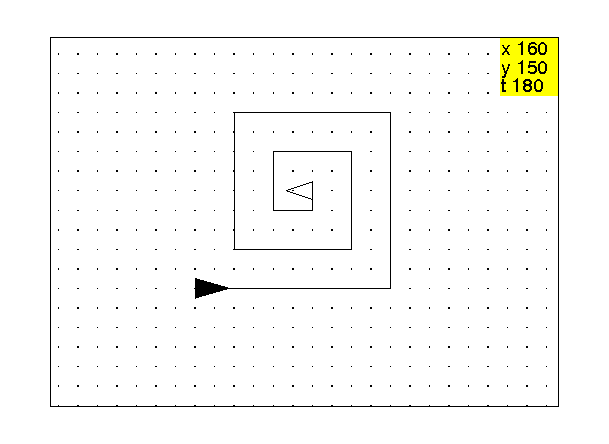
\includegraphics[width=8cm]{tortue0}\end{center}

\subsection{Pour faire une boucle en utilisant la r\'ecursivit\'e}
Une proc\'edure r\'ecursive est une proc\'edure qui s'appelle elle-m\^eme mais
avec des param\`etres diff\'erents et comporte un test d'arr\^et qui permet 
d'interrompre cet appel.\\
On tape dans un \'editeur de programmes puis on compile en appuyant sur {\tt OK}
ou sur {\tt F9} :
\begin{verbatim} 
polygo(n,p,a):={
 si p!=0 alors
   avance(a);
   tourne_gauche(360/n);
   polygo(n,p-1,a);
 fsi;
}:;
\end{verbatim}
Ou on tape en utilisant {\tt si...alors...fsi} au lieu de {\tt if...\{...\}} :
\begin{verbatim} 
polygo(n,p,a):={
 si (p!=0) alors
   avance(a);
   tourne_gauche(360/n);
   polygo(n,p-1,a);
 fsi;
};
\end{verbatim}
Ou on tape une proc\'edure non r\'ecursive en utilisant {\tt repete} :
\begin{center}{\tt polygo(n,p,a):=repete(p,avance(a),tourne\_gauche(360/n))}\end{center}
Puis on tape dans un niveau de l'\'ecran tortue :
\begin{center}{\tt efface;dessine\_tortue;polygo(6,5,50)}\end{center}
On obtient :
\begin{center}{\tt Les 5 cot\'es d'un hexagone de c\^ot\'es 50}\end{center}
\begin{center}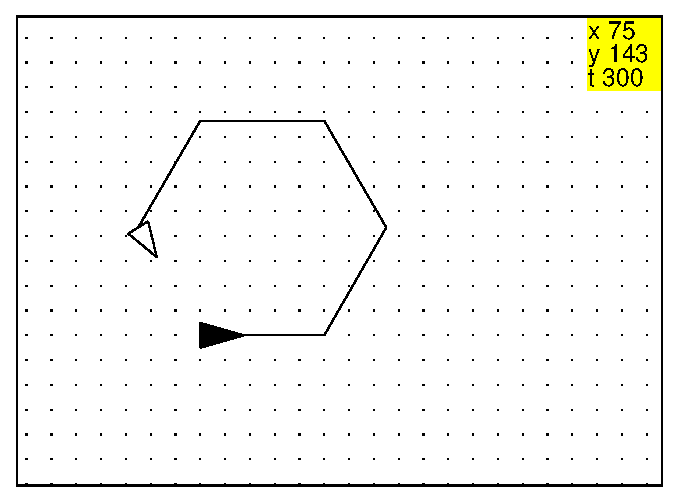
\includegraphics[width=6cm]{tortueh}\end{center}
On veut faire une suite de $n$ triangles \'equilat\`eraux : le premier a pour 
c\^ot\'es $a$, le deuxi\`eme a pour sommet les milieux des cot\'es du premier 
triangle etc ...
On suppose que la tortue a comme position de d\'epart :
un sommet du premier triangle et est dirig\'ee selon un cot\'e et que 
les triangles sont situ\'es sur sa gauche (si vous choisissez les triangles 
sont situ\'es sur sa droite, il suffira de changer les {\tt tourne\_droite} en
{\tt tourne\_gauche} et vice-versa). On choisit la m\^eme position comme 
position d'arriv\'ee.\\
Voici deux proc\'edures r\'ecursives.\\
On dessine le premier triangle, puis on place la tortue \`a l'endroit o\`u il
faut \^etre pour faire l'appel r\'ecursif, on fait l'appel r\'ecursif,
et on ramene la tortue \`a sa position de d\'epart.\\
On tape par exemple dans un \'editeur de programmes puis on compile en appuyant
sur {\tt OK} ou sur {\tt F9} :
\begin{verbatim}
tria(n,a):={
si n!=0 alors 
repete(3,avance(a),tourne_gauche(120));
avance(a/2);
tourne_gauche(60);
tria(n-1,a/2);
tourne_droite(60);
avance(-a/2);
fsi;
}:;
\end{verbatim}
On tape :\\
{\tt efface;dessine\_tortue;tria(5,100)}\\
On obtient :
\begin{center}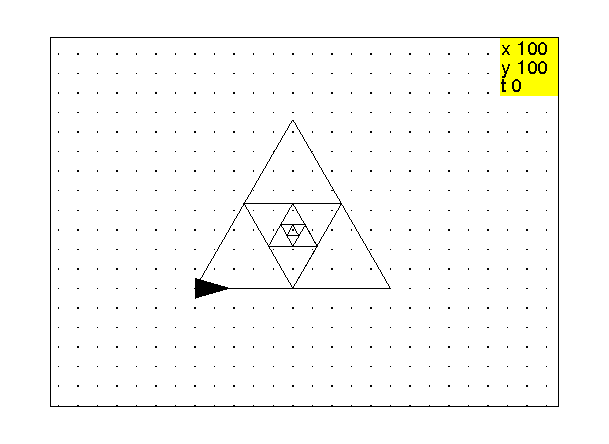
\includegraphics[width=10cm]{tortuet}\end{center}

Ou pour ne pas repasser sur le m\^eme trait, on commence \`a dessiner le 
d\'ebut du premier triangle, puis on place la tortue \`a l'endroit o\`u il faut
\^etre pour faire l'appel r\'ecursif,  on fait l'appel r\'ecursif, puis on 
finit de dessiner le premier triangle et on ram\`ene la tortue \`a sa position 
de d\'epart.\\
On tape :
\begin{verbatim} 
tria1(n,a):={
si n!=0 alors
avance(a/2);
tourne_droite(60);
tria1(n-1,a/2);
tourne_gauche(60);
avance(a/2);
tourne_droite(120);
repete(2,avance(a),tourne_droite(120));
fsi;
}:;
\end{verbatim}
Puis on tape :
\begin{center}{\tt efface;dessine\_tortue;tria1(5,100)}\end{center}
On obtient :
\begin{center}{\tt 5 triangles \'equilat\`eraux, le deuxi\`eme triangle a pour sommet les milieux des cot\'es du premier triangle etc ...}\end{center}
c'est \`a dire le m\^eme dessin que pr\'ec\'edemment.

\subsection{Pour d\'efinir une fonction : {\tt retourne}}\index{retourne}
\noindent {\tt retourne} a un argument qui est la valeur que l'on veut donner 
\`a la fonction.\\
{\tt retourne} permet d'interrompre le programme et de renvoyer l'argument 
de {\tt retourne} comme \'etant la valeur de la fonction que l'on d\'efinit.\\
On tape pour avoir une fonction bool\'eenne qui nous dit si il y a un terme nul dans une liste {\tt l} :
\begin{verbatim}
zerodansl(l):={
 pour k de 0 jusque size(l)-1 faire 
  si l[k]==0 alors 
  retourne(1);
  fsi; 
 fpour; 
 retourne(0);
}:;
\end{verbatim}
Ou on tape :\\
\begin{verbatim}
zeroinl(l):={
 for (k:=0;k<size(l);k++){
  if (l[k]==0) retourne(1);
 } 
 retourne(0);
 }:;
\end{verbatim}
On obtient :
\begin{center}{\tt La fonction bool\'eenne qui teste si il y a un z\'ero dans 
une liste}\end{center}
{\bf Remarque}\\
Lorsqu'on fait un dessin tortue, on \'ecrit une proc\'edure : cette proc\'edure
va ex\'ecuter toutes les instructions graphiques et renvoie automatiquement 
l'\'etat de la tortue. On n'a donc pas besoin d'utiliser {\tt retourne}, sauf 
si on a besoin de transmettre un r\'esultat.

\subsection{Pour lire une expression\`a partir du clavier : {\tt lis}}\index{lis}
\noindent {\tt lis} a un argument qui est le nom d'une variable.\\
{\tt lis} interrompt le programme et ouvre une petite fene\^etre qui permet 
d'entrer une expression qui sera la valeur de l'argument de {\tt lis} : si 
l'expression est une cha\^{\i}ne de caract\`eres il faut mettre des 
guillemets.\\
On tape :
\begin{verbatim}
pilote(l):={
si l==f alors retourne 1;fsi; 
si l==e alors L:=L,"efface";efface; fsi;
si l==a alors avance; fsi;
si l==r alors recule; fsi;
si l==d alors tourne_droite; fsi;
si l==g alors tourne_gauche; fsi;
lis(l);
pilotee(l);
}:;
\end{verbatim}
Puis on tape :
\begin{center}{\tt pilote(a) d a d a d a f}\end{center}
On obtient :
\begin{center}{\tt un carr\'e}\end{center}
Si on veut garder les instructions qui ont \'et\'e ex\'ecut\'ees, On peut  
renvoyer une chaine de caract\`eres contenant ces instructions separ\'ees par 
des {\tt ;}.\\
On tape :
\begin{verbatim}
piloter(l):={
local L;
si l==f alors retourne "";fsi; 
si l==e alors L:="efface;";efface; fsi;
si l==a alors L:="avance;";avance; fsi;
si l==r alors L:="recule;";recule; fsi;
si l==d alors L:="tourne_droite;";tourne_droite; fsi;
si l==g alors L:="tourne_gauche;";tourne_gauche; fsi;
lis(l);
retourne L+piloter(l);
}:;
\end{verbatim}
Puis on tape :
\begin{center}{\tt A:=piloter(a)}\end{center}
Puis :
\begin{center}{\tt d a d a d a f}\end{center}
On obtient :
\begin{center}{\tt un carr\'e}\end{center}
Puis on tape :
\begin{center}{\tt A}\end{center}
On obtient :
\begin{center}{\tt "avance;tourne\_droite;avance;tourne\_droite;\\
  avance;tourne\_droite;avance;tourne\_droite"}\end{center}
Puis on tape :
\begin{center}{\tt efface;execute(A)}\end{center}
On obtient \`a nouveau :
\begin{center}{\tt un carr\'e}\end{center}

\subsection{Pour lire une cha\^{\i}ne de caract\`eres \`a partir du clavier : {\tt lis\_phrase}}\index{lis\_phrase}
\noindent {\tt lis\_phrase} a un argument qui est le nom d'une variable.\\
{\tt lis\_phrase} interrompt le programme et ouvre une petite fene\^etre qui 
permet d'entrer une cha\^{\i}ne de caract\`eres qui sera la valeur de 
l'argument de {\tt lis\_phrase} : on tape la cha\^{\i}ne de caract\`eres sans
mettre les guillemets.\\
On tape :
\begin{verbatim}
conduite(l):={
si l=="f" alors retourne 1;fsi; 
si l=="e" alors efface; fsi;
si l=="a" alors avance fsi;
si l=="r" alors recule fsi;
si l=="d" alors tourne_droite; fsi;
si l=="g" alors tourne_gauche; fsi;
lis_phrase(l);
conduite(l);
}:;
\end{verbatim}
Puis on tape :
\begin{center}{\tt conduite("a") d a d a d a f}\end{center}
On obtient :
\begin{center}{\tt un carr\'e}\end{center}
Si on veut garder la suite des instructions qui a \'et\'e ex\'ecut\'ee, on peut
renvoyer une chaine de caract\`eres contenant ces instructions separ\'ees par 
des {\tt ;}.\\
On tape :
\begin{verbatim}
conduire(l):={
local L;
si l=="f" alors retourne "";fsi; 
si l=="e" alors L:="efface;";efface; fsi;
si l=="a" alors L:="avance;";avance; fsi;
si l=="r" alors L:="recule;";recule; fsi;
si l=="d" alors L:="tourne_droite;";tourne_droite; fsi;
si l=="g" alors L:="tourne_gauche;";tourne_gauche; fsi;
lis_phrase(l);
retourne L+conduire(l);
}:;
\end{verbatim}
Puis on tape :
\begin{center}{\tt A:=conduire("a") d a d a d a f}\end{center}
On obtient :
\begin{center}{\tt un carr\'e}\end{center}
Puis on tape :
\begin{center}{\tt A}\end{center}
On obtient :
\begin{center}{\tt "avance;tourne\_droite;avance;tourne\_droite;\\
  avance;tourne\_droite;avance;tourne\_droite"}\end{center}
Puis on tape :
\begin{center}{\tt  efface;execute(A)}\end{center}
On obtient \`a nouveau :
\begin{center}{\tt un carr\'e}\end{center}

\subsection{Pour ex\'ecuter une cha\^{\i}ne de caract\`eres : {\tt execute}}\index{execute}
\noindent {\tt execute} a comme argument cha\^{\i}ne de caract\`eres qui est 
une suite de commande. L'argument doit \^etre mis entre des parenth\`eses\\
{\tt execute} ex\'ecute cette suite de commande.\\
On tape :\\
\begin{center}{\tt execute(" tourne\_droite;avance 40; rectangle\_plein(20,40);avance -40")}\end{center}
On obtient :
\begin{center}{\tt le dessin d'un "drapeau"}\end{center}

\section{Faire un dessin pas \`a pas en le m\'emorisant}
\subsection{Pour enregistrer les commandes : {\tt debut\_enregistrement}}\index{debut\_enregistrement}
\noindent {\tt debut\_enregistrement} a comme argument un nom de proc\'edure.\\
{\tt debut\_enregistrement} va permettre d'enregistrer les commandes comprises 
entre {\tt debut\_enregistrement} et {\tt fin\_enregistrement} et ainsi
d\'efinir une proc\'edure du nom donn\'e en argument de 
{\tt debut\_enregistrement}.\\
On tape :
\begin{center}{\tt tourne\_gauche }\end{center}
\begin{center}{\tt debut\_enregistrement(arbre)}\end{center}
Puis on tape les instructions pour d\'efinir {\tt arbre} par exemple :
\begin{center}{\tt avance 50}\end{center}
Puis
\begin{center}{\tt disque\_centre 20}\end{center}
Puis
\begin{center}{\tt recule 40}\end{center}
Puis on termine  l'enregistrement avec :
\begin{center}{\tt fin\_enregistrement("arbre.tor")}\end{center}
On obtient :
\begin{center}{\tt Un fichier arbre.tor qui content les instructions d'une 
proc\'edure qui a comme nom arbre}\end{center}
On tape :
\begin{center}{\tt efface;tourne\_gauche;}\end{center}
\begin{center}{\tt arbre()}\end{center}
On obtient :
\begin{center}{\tt Le dessin de n\^otre arbre}\end{center}

\subsection{Pour terminer l'enregistrement : {\tt fin\_enregistrement}}\index{fin\_enregistrement}
\noindent {\tt fin\_enregistrement} a comme argument une chaine de caract\`eres.\\
{\tt fin\_enregistrement} sauve la proc\'edure d\'efinie par les instructions 
comprises entre {\tt debut\_enregistrement} et {\tt fin\_enregistrement}
dans le fichier dont le nom est pass\'e en argument de {\tt fin\_enregistrement}.\\
On tape :
\begin{center}{\tt debut\_enregistrement(arbre)}\end{center}
Puis on tape les instructions pour d\'efinir {\tt arbre}, puis on tape :
\begin{center}{\tt fin\_enregistrement("arbre.tor")}\end{center}
On obtient :
\begin{center}{\tt Le fichier arbre.tor contenant la proc\'edure arbre}\end{center}
\section{Faire un dessin en \'ecrivant une proc\'edure}
\noindent On peut \'ecrire une proc\'edure dans l'\'editeur de programmes.\\
On tape les instructions pour d\'efinir {\tt arbre} par exemple :
\begin{verbatim}
arbre():={
 avance 50;
 disque_centre 20;
 recule 40;
}:;
\end{verbatim}
Puis on tape :
\begin{verbatim}
tourne_gauche;
dessine_tortue;
arbre()
}:;
\end{verbatim}
On obtient :
\begin{center}{\tt Le dessin qui a comme nom arbre : on remarque que la tortue n'est pas revenue \`a sa position de d\'epart}\end{center}
\begin{center}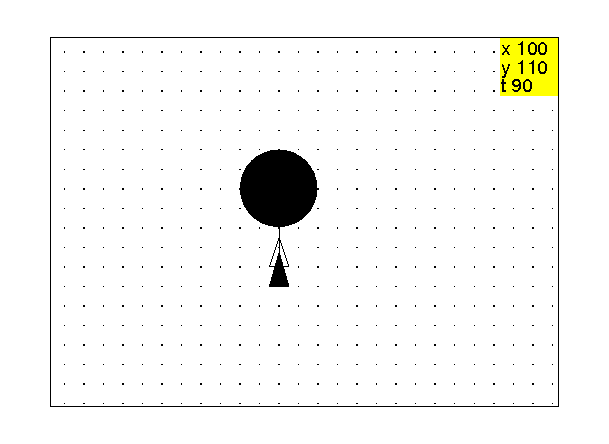
\includegraphics[width=\textwidth]{tortuea}\end{center}
On tape les instructions pour d\'efinir {\tt arbre} avec deux param\`etres :
\begin{verbatim}
arbres(a,b):={
 avance a;
 disque_centre b;
 recule 2*b;
}:;
\end{verbatim}
Puis on tape :
\begin{center}{\tt efface;tourne\_gauche;dessine\_tortue;arbres(50,20)}\end{center}
On obtient :
\begin{center}{\tt Le dessin pr\'ec\'edent }\end{center}

\section{Mettre et retrouver des proc\'edures dans un fichier}
\subsection{\'Ecrire des proc\'edures dans un fichier : {\tt sauve}}\index{sauve}
\noindent {\tt sauve} a comme argument une cha\^{\i}ne de caract\`eres qui est 
le nom d'un fichier et le nom des proc\'edures et des variables que l'on veut 
sauver dans ce fichier.\\
{\tt sauve} permet de mettre en m\'emoire ces proc\'edures dans ce fichier
et donc de pouvoir les r\'eutiliser dans une autre session de travail.\\
On tape :
\begin{center}{\tt sauve("toto.tor",tete,bras)}\end{center}
On obtient :
\begin{center}{\tt le fichier "toto.tor" contenant les proc\'edures tete et bras}\end{center}
On tape :
\begin{center}{\tt sauve("toto.tor",tete,bras)}\end{center}
On obtient :
\begin{center}{\tt le fichier "toto.tor"contenant les proc\'edures tete et bras}\end{center}

\subsection{Utiliser les proc\'edures \'ecrites dans un fichier : {\tt ramene}}\index{ramene}
\noindent {\tt ramene} a comme argument une cha\^{\i}ne de caract\`eres qui 
est le nom d'un fichier contenant des proc\'edures agissant sur la tortue.\\
{\tt ramene} permet de valider et donc d'utiliser les proc\'edures 
se trouvant dans ce fichier.\\
On tape :
\begin{center}{\tt ramene("toto.tor")}\end{center}
On obtient :
\begin{center}{\tt la validation des proc\'edures tete et bras}\end{center}


\chapter{Pour g\'erer l'espace de travail}

\section{Pour d\'emarrer}
Ouvrir un \'ecran {\tt dessin tortue} ({\tt Alt+d}), et \'eventuellement un 
\'editeur de programmes ({\tt Alt+p}).

\section{Pour conserver votre travail en fin de session}
Pour conserver tout le contenu de votre feuille en fin de session il faut
utiliser le menu {\tt Fich}, et cliquer sur {\tt sauver} ou 
{\tt sauver comme} (vous pouvez choisir le nom du fichier de sauvegarde
d'extension {\tt .xws}). 
Vous avez ainsi un fichier archive d'extension {\tt .xws}.

\section{Pour retrouver le travail de la session pr\'ec\'edente}
Pour retrouver le travail de la session pr\'ec\'edente et mettre son contenu 
dans votre feuille de calcul, il faut utiliser le menu {\tt Fich}, et cliquer 
sur {\tt Charger} puis mettre le nom du fichier de sauvegarde

\section{Pour \'ecrire et sauver des proc\'edures}
On peut \'ecrire des proc\'edures dans son \'editeur pr\'ef\'er\'e ou dans 
un \'editeur de programmes de {\tt Xcas} ou encore avec les commandes 
{\tt debut\_enregistrement} et {\tt fin\_enregistrement}.\\
Lorsque votre programme est dans un \'editeur de programmes ouvert avec 
{\tt Alt+p}, vous pouvez valider votre programme avec le 
bouton {\tt OK}. Si il y a une erreur, on vous donne la ligne o\`u elle se 
trouve dans les messages et cette ligne est en surbrillance dans l'\'editeur 
de programmes (attention l'erreur se trouve quelquefois \`a la fin de la ligne 
pr\'ec\'edente par exemple si il manque ;). Si il n'y a pas d'erreur, on vous 
dit {\tt Success} la ligne dans les messages. Lorsqu'on vous clique sur
le bouton {\tt save} de l'\'editeur de programmes, on vous propose un 
nom pour le sauver : ce nom sera par defaut  {\tt session0.cxx} puis 
{\tt session1.cxx} etc...\\
{\bf Conseil :}  donner un nom aux fichiers que vous voulez conserver !


On peut aussi d\'efinir des proc\'edures en recopiant, dans un \'editeur de 
programmes ouvert avec {\tt Alt+p}, les commandes qui se sont
inscritent dans l'enregistreur qui est le petit \'editeur de programmes 
attach\'e \`a l\'ecran tortue
lors de la confection d'un dessin. Cela permet de mettre au
point une proc\'edure car on peut modifier son contenu en supprimant les faux 
pas ou en rajoutant des commandes et refaire 
l'execution de ce qui s'y trouve : puisque les commandes  d\'ebutent par 
{\tt efface;}, il suffit de mettre mettre le cuseur dans l'enregistreur (petit 
\'editeur de programmes attach\'e \`a la tortue),
puis, de s\'electionner le menu {\tt Edit-> Executer tout} de l'enregistreur
ou d'appuyer sur {\tt F7} (voir aussi \ref{sec:enregis}).

On peut aussi d\'efinir des proc\'edures en enregistrant les commandes quand on 
fait du pas \`a pas en utilisant {\tt debut\_enregistrement} et 
{\tt fin\_enregistrement} : ainsi de jeunes enfants peuvent d\'efinir 
facilement des proc\'edures.

\section{Pour utiliser des proc\'edures sauv\'ees pr\'ec\'edement}
\noindent Pour utiliser des proc\'edures sauv\'ees pr\'ec\'edement il faut 
utiliser la commande {\tt ramene}.\\
On tape, pour valider les proc\'edures se trouvant dans le fichier 
{\tt "toto.cxx"}:\\
\begin{center}{\tt ramene("toto.cxx")}\end{center}
On obtient \'ecrit en bleu :
\begin{center}{\tt //Parsing toto //Success compiling toto etc...}\end{center}
On obtient en noir :
\begin{center}{\tt la d\'efinition des proc\'edures contenues dans toto.cxx}\end{center}
\section{Pour connaitre les noms des proc\'edures utilisables}\index{VARS}\index{sommet}\index{'program'}
Pour connaitre les noms des proc\'edures pr\'esentes dans votre espace de 
travail il faut taper {\tt VARS}  : cela donne les noms des proc\'edures 
valides et des variables affect\'ees.
0n tape :
\begin{center}{\tt a:=30;c(b):=\{avance(b);tourne\_droite;\}}\end{center}
Puis on tape :
\begin{center}{\tt VARS}\end{center}
On obtient :
\begin{center}{\tt [a,c]}\end{center}
On peut tester si c'est un programme en utilisant :\\
{\tt sommet(c)=='program'} 
0n tape :
\begin{center}{\tt sommet(c)=='program'}\end{center}
On obtient :
\begin{center}{\tt 1}\end{center}
0n tape :
\begin{center}{\tt sommet(a)=='program'}\end{center}
On obtient :
\begin{center}{\tt 0}\end{center}


\section{Pour voir les instructions d\'efinissant une proc\'edure}
Pour connaitre les instructions d\'efinissant une proc\'edure, il suffit de 
taper le nom de cette proc\'eduredans une ligne d'entr\'ee de commandes : la 
d\'efinition de la proc\'edure s'affiche alors dans la zone des r\'eponses.\\
Pour connaitre la valeur d'une variable, il suffit de 
taper son nom dans une ligne d'entr\'ee de commandes : la valeur de la 
variable s'affiche alors dans la zone des r\'eponses.\\
Puisque les sorties de la  ligne d'entr\'ee de  la tortue ne sont prevues que
pour afficher une seule ligne, il est pr\'ef\'erable de taper le nom d'une 
proc\'edure dans une ligne d'entr\'ee de commandes de {\tt Xcas}.


\section{Pour effacer des fichiers}
Il faut effacer les fichiers depuis l'\'ecran {\tt xterm} (sous Linux) et 
employer la commande {\tt rm}.
0n tape par exemple :
\begin{center}{\tt rm titi.tor}\end{center}
On obtient :
\begin{center}{\tt rm: d\'etruire fichier r\'egulier `titi.tor'?}\end{center} 
Le fichier sera d\'etruit si on tape sur {\tt enter} et non d\'etruit si on 
r\'epond  {\tt n enter}.

\section{Pour imprimer vos dessins}
{\tt Imprimer} du menu de {\tt Menu} de la barre de boutons de l'\'ecran 
{\tt Tortue} imprime le dessin situ\'e sur cet \'ecran ou transforme cet 
\'ecran en un fichier LaTex ({\tt Pr\'evisualiser avec LaTex}).\\ 
Vous pouvez ainsi obtenir deux fichiers :\\
-  un fichier LaTex d'extension {\tt .tex} (que vous pouvez compiler et 
imprimer ou encore ins\'erer en enlevant l'en t\^ete et la 
derni\`ere ligne dans un autre fichier LaTex),\\
- un fichier postscript d'extension {\tt .ps} (que vous pouvez imprimer)


\section{Pour arr\^eter}
V\'erifier que vous avez sauv\'e ce que vous voulez conserver.\\
Cliquer sur le menu {\tt Session}, selectionner  {\tt Quitter}. 


\chapter{Des activit\'es en CP, CE1 et CE2}
Le CP est le cours pr\'eparatoire destin\'e aux enfants de 6 ans environ.\\
Le CE1 et le CE2 sont les cours elementaires premi\`ere et deuxi\`eme ann\'ee
destin\'es aux enfants de 7-8 ans environ.
\section{Des dessins en pas \`a pas}
On utilise ici les commandes {\tt avance}, {\tt tourne\_droite} et 
{\tt tourne\_gauche}. \\
L'enfant utilise les boutons de la barre des boutons :\\
{\tt av} ou  {\tt td} ou {\tt tg} qui \'ecrivent {\tt avance} ou
{\tt tourne\_droite} ou {\tt tourne\_gauche} dans la ligne de commande.\\
Dans les dessins de cette section, il s'agit de reconnaitre la gauche de la 
droite de la tortue. Pour les enfants qui sont en dificult\'e on peut tracer 
sur un morceau de papier calque une fl\`eche, o\`u l'on marque {\tt D} sur le
cot\'e droit et {\tt G} sur le cot\'e gauche, par exemple :

%\input figtortue/fleche.tex
\begin{center}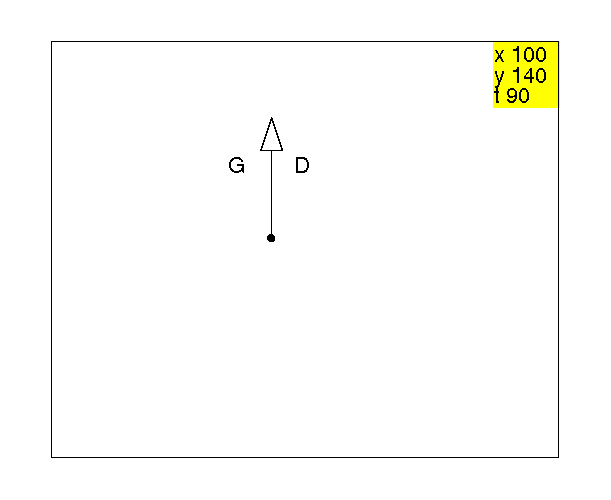
\includegraphics[width=10cm]{tortuef}\end{center}

On explique que la fl\`eche c'est la t\^ete de la tortue et que le point c'est 
l\`a o\`u elle se trouve, et quand elle tourne, elle reste \`a la m\^eme place 
et seule sa t\^ete change de direction.  
\subsection{Faire un escalier en pas \`a pas}
Sur un papier quadrill\'e ou sur du papier point\'e, l'enfant dessine 
l'escalier de 4 marches ci-dessous :

%file escalier
% Generated by xcas
%segment(-3-3*i,-3-2*i);segment(-3-2*i,-2-2*i);
%segment(-2-2*i,-2-i);segment(-2-i,-1-i);segment(-1-i,-1);
%segment(-1,0);segment(0,1);segment(1,1+i);
%\input figtortue/escalier.tex
\begin{center}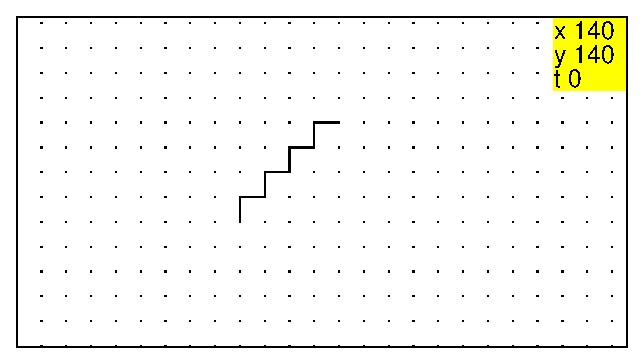
\includegraphics[width=10cm]{tortuee}\end{center}

Puis il doit reproduire ce dessin sur l'\'ecran de l'ordinateur.\\
L'enfant utilise les boutons {\tt av} ou {\tt td} ou {\tt tg}, puis appuie 
sur {\tt entree} : il ne pr\'evoit pas \`a l'avance les commandes mais il 
travaille au pas \`a pas.\\
Dans un deuxi\`eme temps on pourra ex\'ecuter plusieurs commandes en 
les s\'eparant par {\tt ;} par exemple :
{\tt avance;tourne\_droite; avance;tourne\_gauche;}
\subsection{Faire descendre l'escalier \`a la tortue}
Une fois l'escalier termin\'e on peut lui demander de faire revenir la tortue 
\`a son point de d\'epart en passant sur les traits : ce dessin se fera en 
utilisant une autre couleur.\\
L'enfant utilise les boutons {\tt cr} puis {\tt av} ou {\tt td} ou {\tt tg}, 
puis appuie sur {\tt entree}.\\
 {\tt cr} est l'abreviation de la commande {\tt crayon} qui permet de changer 
la couleur du crayon par exemple : {\tt crayon rouge} ou {\tt crayon gomme}.
\subsection{Faire deux escaliers sym\'etriques}
L'enfant peut utiliser les boutons {\tt av}, {\tt re}, {\tt td} et {\tt tg}, 
abreviations des commandes 
{\tt avance, recule, tourne\_gauche, tourne\_droite}.\\
Ici, on remarquera que le symetrique s'obtient avec la m\^eme suite de 
commandes que celle utilis\'ee pour faire le premier escalier.\\ 
\begin{center}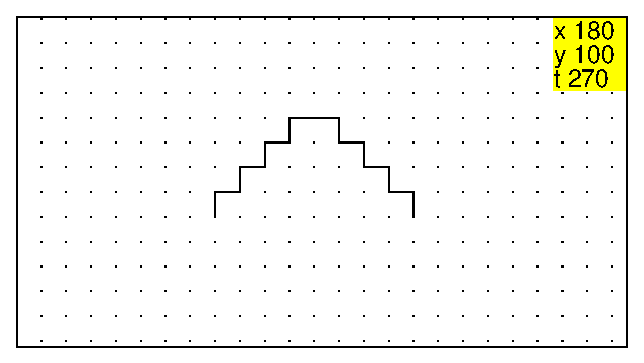
\includegraphics[width=\textwidth]{tortuee2}\end{center}
\subsection{Faire une tour et un chateau fort}
Sur un papier point\'e, l'enfant dessine la tour et le chateau fort suivants :\\
%\input figtortue/tour.tex
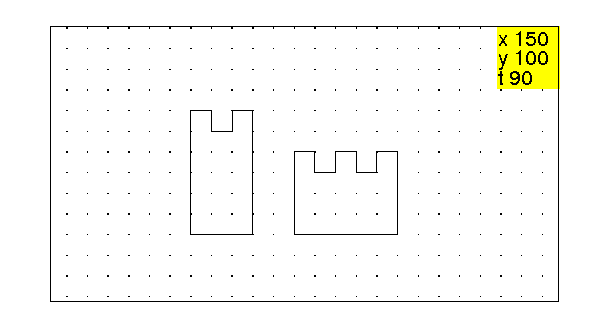
\includegraphics[width=\textwidth]{tortuetch} 
Puis il doit reproduire ce dessin sur l'\'ecran de l'ordinateur.

\subsection{Faire un chateau et deux tours}
Durant cette s\'eance, il faut faire comprendre que les commandes pour 
r\'ealiser la deuxi\`eme tour seront les m\^emes que celles de la premi\`ere 
tour \`a condition de mettre la tortue au bon endroit au demarrage du trac\'e
 de la deuxi\`eme tour.

\begin{center}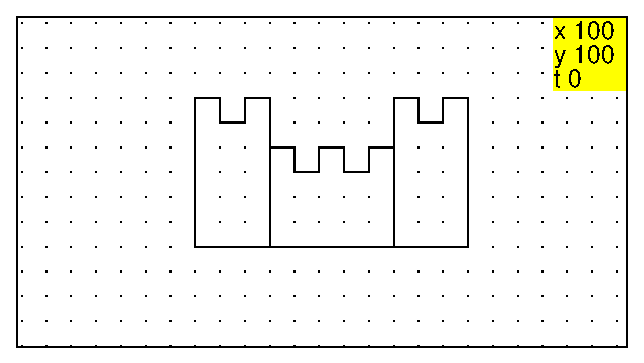
\includegraphics[width=\textwidth]{tortuech}\end{center}

\section{Cr\'eation de nouvelles commandes}
On explique  que l'on peut donner un nom \`a une suite de commandes en
 utilisant les commandes {\tt debut\_enregistrement} et 
{\tt fin\_enregistrement}
\subsection{M pour faire une marche d'escalier}
La proc\'edure {\tt M} va r\'ealiser le dessin ci-dessous sur lequel on a 
not\'e \`a l'aide d'un triangle plein la position de d\'epart de la tortue et
 par un triangle la position d'arriv\'ee de la tortue.
% Generated by xcas marche.tex
%\input figtortue/marche.tex\end{center}
\begin{center}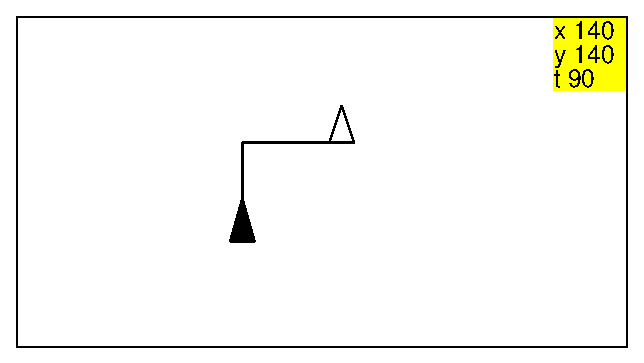
\includegraphics[width=\textwidth]{tortuem}\end{center}
On tape par exemple :\\
{\tt debut\_enregistrement "M"} puis,\\
{\tt avance entr\'ee}\\
{\tt tourne\_droite entr\'ee}\\ 
{\tt avance entr\'ee}\\
{\tt tourne\_gauche entr\'ee} puis,\\
{\tt fin\_enregistrement "M.cxx"}\\
On vient ainsi de cr\'eer deux choses :\\
la commande {\tt M()} qui dessine une marche et le fichier {\tt M.cxx} qui 
contient cette commande : on pourra ainsi retrouver la commande {\tt M} lors des s\'eances suivantes en tapant :\\
{\tt ramene "M.cxx"}.\\
 {\bf Attention} \\
- les noms des fichiers sont entour\'es de {\tt "} mais pas 
le nom de la commande.
- pour ex\'ecuter la commande il est obligatoire de faire suivre le nom par des
 parenth\`eses comme : {\tt M()}.
- une commande r\'ealise un dessin d\'ependant de la position de la tortue
avant son ex\'ecution (position de d\'epart) et qui laisse la tortue en 
g\'en\'eral \`a un autre endroit (position finale).\\
Il faut comprendre que les deux dessins ci-dessous sont le r\'esultat de 
l'ex\'ecution de la m\^eme proc\'edure {\tt M()} car les dessins sont 
superposables et se font selon la position de la tortue au d\'epart.
\begin{center}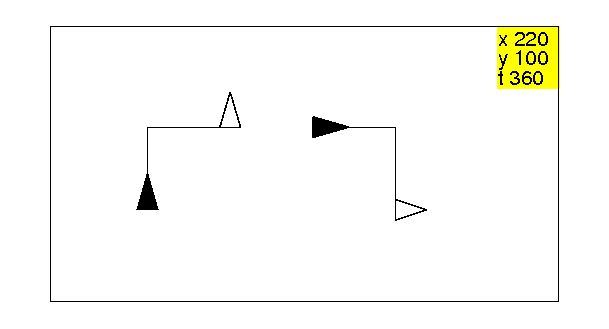
\includegraphics[width=\textwidth]{tortuem2}\end{center}

{\bf Exemple : l'escalier sym\'etrique}\\
On tape :\\
{\tt M();M();M();M(); entr\'ee} puis,\\
{\tt tourne\_droite; entr\'ee}\\
{\tt M();M();M();M(); entr\'ee}\\
Avec des \'el\`eves plus ag\'es on peut \'ecrire directement :\\
{\tt M():=\{avance;tourne\_droite;avance;tourne\_gauche;\}},
puis pour avoir le dessin de l'escalier :\\
{\tt tourne\_gauche;repete(4,M())}

On peut aussi \'ecrire la proc\'edure {\tt escalier} ayant comme param\`etre
{\tt n}, le nombre de marches :\\
{\tt escalier(n):=repete(n,M())}.\\
On a alors :\\
{\tt escalier2(n):=\{escalier(n); tourne\_droite;escalier(n)\}}
puis pour avoir le dessin de l'escalier sym\'etrique ayant 7 marches:\\
{\tt tourne\_gauche; escalier2(7)}
\subsection{T pour faire une tour}
La proc\'edure {\tt T} va r\'ealiser le dessin ci-dessous sur lequel on a 
not\'e \`a l'aide d'un triangle plein la position de d\'epart de la tortue et
 par un triangle la position d'arriv\'ee de la tortue : ici on ne voit qu'un 
triangle plein car la position d'arriv\'ee  de la tortue est la m\^eme que sa 
position de d\'epart.
% Generated by xcas tour2.tex
%\input figtortue/tour2.tex\\
\begin{center}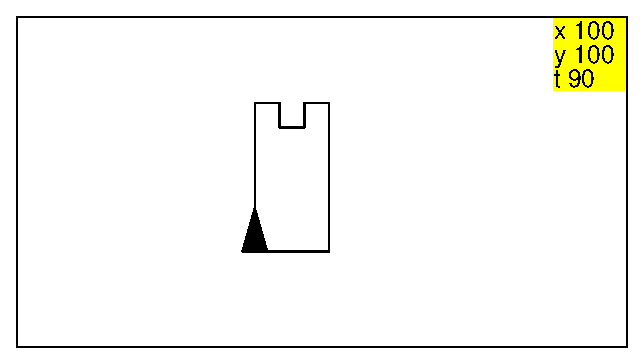
\includegraphics[width=\textwidth]{tortuett}\end{center}
{\bf Remarque}\\
Il faut bien voir que l'\'ecriture de la proc\'edure {\tt T} d\'epend du choix
de la position de d\'epart et d'arriv\'ee de la tortue et que pour un m\^eme 
dessin il y a plusieurs choix possibles.\\ 
On tape :\\
{\tt debut\_enregistrement "T"} puis,\\
{\tt avance(60) entr\'ee}\\
{\tt tourne\_droite entr\'ee}\\ 
{\tt avance entr\'ee}\\
{\tt tourne\_droite entr\'ee}\\ 
{\tt avance entr\'ee}\\
{\tt tourne\_gauche entr\'ee}\\
{\tt avance entr\'ee}\\
{\tt tourne\_gauche entr\'ee}\\
{\tt avance entr\'ee}\\
{\tt tourne\_droite entr\'ee}\\ 
{\tt avance entr\'ee}\\
{\tt tourne\_droite entr\'ee}\\ 
{\tt avance(60) entr\'ee}\\
{\tt tourne\_droite entr\'ee}\\ 
{\tt avance(30) entr\'ee}\\
{\tt tourne\_droite entr\'ee}\\ 
{\tt fin\_enregistrement "M.cxx"}\\
Puis on tape :\\
{\tt tourne\_gauche entr\'ee}\\
{\tt T() entr\'ee}
\subsection{Pour faire plusieurs tours}
Pour faire plusieurs tours, on tape :\\
{\tt tourne\_gauche entr\'ee}\\
{\tt T() entr\'ee}
{\tt pas\_de\_cote -30 entr\'ee}
{\tt T() entr\'ee}
{\tt pas\_de\_cote -30 entr\'ee}
{\tt T() entr\'ee} etc...
\section{Le dessin d'un train}
Ce train est compos\'e d'une locomotive {\tt L}, de wagons de voyageurs  
{\tt V} et de  wagons de marchandises {\tt W}.\\

Pour faire {\tt L},{\tt V} et {\tt W} on a besoin de savoir faire un carr\' e
{\tt C}.
Les proc\'edures {\tt C}, {\tt L}, {\tt V} et {\tt W} vont r\'ealiser le dessin 
ci-dessous sur lequel on a 
not\'e \`a l'aide d'un triangle plein la position de d\'epart de la tortue et
\`a l'aide d'un triangle sa position d'arriv\'ee.\\
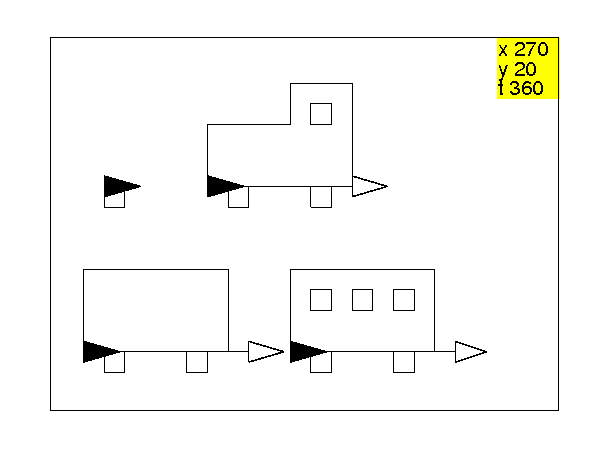
\includegraphics[width=\textwidth]{tortuew}\\
On tape :
\begin{verbatim}
C():={
repete(4,avance,tourne_droite);
 }:;
W():={
avance ;C();
avance 40;C();
avance 20;
tourne_gauche ;
avance 40;
tourne_gauche ;
avance 70;
tourne_gauche ;
avance 40;
tourne_gauche ;
avance 80;
}:;
V():={
W();
recule 70;
pas_de_cote 30;
repete(3,C(),saute 20);
pas_de_cote -30;
avance;
}:;
L():={
avance 10;C();
avance 40;C();
avance 20;
tourne_gauche ;
avance 50;
tourne_gauche ;
avance 30;
tourne_droite ;
recule 20;
pas_de_cote -10;
C();pas_de_cote ;
tourne_gauche ;
avance 40;
tourne_gauche ;
avance 30;
tourne_gauche ;
avance 70;
}
:;
\end{verbatim}

Un train peut alors se former en tapant :
{\tt  W();V();L()}\\

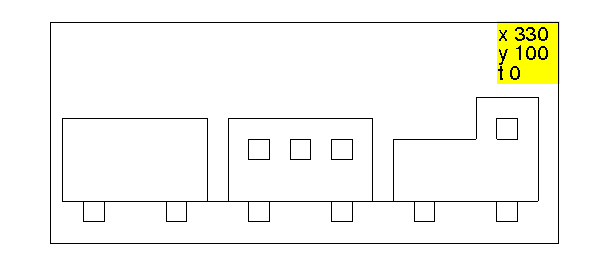
\includegraphics[width=\textwidth]{tortuetrain}
\section{Les frises}
Nous allons apprendre dans cette s\'eance \`a se servir des commandes :\\
{\tt rectangle\_plein, triangle\_plein, disque} et utiliser aussi les commandes
 {\tt repete} pour r\'ep\'eter et {\tt crayon} pour changer la couleur.\\
Nous allons mettre c\^ote \`a cote plusieurs fois le m\^eme motif.\\
Nous choisissons des motifs simples comme par exemple :
un carr\'e, un saut etc...\\
un carr\'e rouge, un carr\'e noir etc...\\
un triangle isoc\`ele rectangle plein, un saut etc...\\
un triangle isoc\`ele rectangle plein rouge, un  isoc\`ele rectangle plein noir etc...\\
un disque, un saut etc...\\
un disque rouge, un disque noir etc...\\
un quart de disque, un saut etc...\\
un quart de disque rouge, un quart de disque noir etc...\\
On pourra  \'ecrire dans la ligne des commandes :\\
{\tt rectangle\_plein 20;saute 40}\\
que l'on peut valider plusieurs fois (il faut savoir aussi que  {\tt Ctrl}+
la fl\`eche vers le haut du clavier met dans la ligne des commandes, les 
commandes pr\'ec\'edentes et que {\tt esc} efface la ligne des commandes).\\
On explique que :\\
{\tt rectangle\_plein 20;saute 40;rectangle\_plein 20;saute 40;}\\
produit la m\^eme chose que :\\
{\tt repete(2,rectangle\_plein 20,saute 40)}\\
Il faut bien faire attention \`a la syntaxe :\\
{\tt ;} s\'epare deux instructions et\\
{\tt ,} s\'epare les param\`etres d'une instruction.\\
On tape par exemple :
\begin{verbatim}
des_tor():={
cache_tortue;
tourne_gauche;
avance 5;
tourne_droite(180-180/pi*atan(3.4));
avance(sqrt(25+17^2));
tourne_droite(180-2*180/pi*atan(1/3.4));
avance(sqrt(25+17^2));
tourne_droite(180-180/pi*atan(3.4));
avance 5;tourne_droite;
montre_tortue;
}:;
motif0():={
crayon vert;
rectangle_plein 20;
crayon jaune;
dessine_tortue;
saute(20);
crayon rouge;
tourne_droite ;
rectangle_plein 20;
tourne_gauche;
saute(20);
}:;
motif():={
crayon vert;
rectangle_plein 20;
saute(20);
crayon rouge;
tourne_droite ;
rectangle_plein 20;
tourne_gauche;
saute(20);
}:;
\end{verbatim}
Puis on tape :
\begin{verbatim}
pas_de_cote -60;
saute -40;
repete(5,motif());
cache_tortue;
\end{verbatim}
On obtient :\\
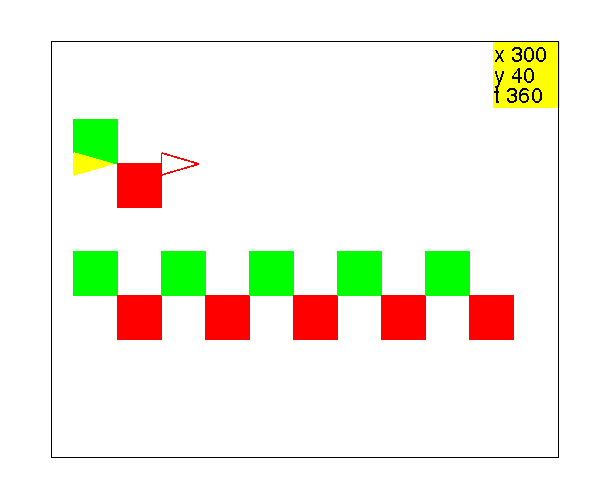
\includegraphics[width=\textwidth]{tortfrise}
\section{Le dessin d'un  bonhomme et d'une ribambelle de bonhommes}
Ici on utilise la commande {\tt rectangle\_plein} qui dessine un carr\'e ou 
un rectangle plein :\\
{\tt rectangle\_plein} dessine un carr\'e plein de c\^ot\'es 10 dans le sens 
trigonom\'etrique.\\
{\tt rectangle\_plein 20} ou {\tt rectangle\_plein(20)} dessine un carr\'e  
plein de c\^ot\'es 20 dans le sens trigonom\'etrique.\\
{\tt rectangle\_plein(20,50)} dessine un rectangle plein de 
c\^ot\'es 20 et 50 dans le sens trigonom\'etrique.\\
{\bf Attention}
Les parenth\`eses sont onligatoires pour les primitives ayant plus d'un 
param\`etre.\\
Voici la ribambelle de bonhommes que l'on veut dessiner :\\
% Generated by xcas bonhom.tex
%\input figtortue/bonhom.tex
 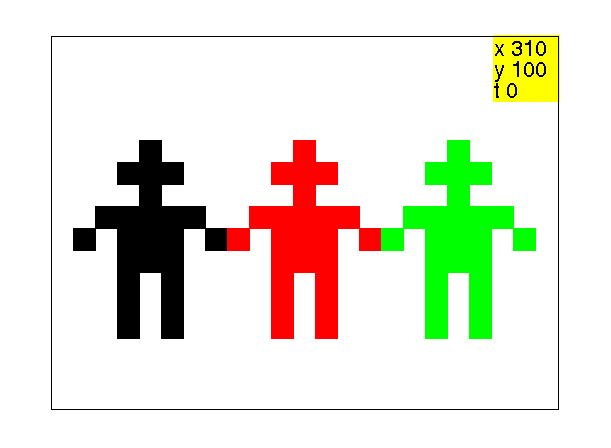
\includegraphics[width=\textwidth]{tortbon}
On va \'ecrire une proc\'edure {\tt bonhomme}. Il faut bien comprendre que les 
choix du d\'epart et d'arriv\'ee de la tortue ne sont pas uniques et dependent 
de ce que l'on veut faire par 
exemple, pour faire une ribambelle il 
peut \^etre judicieux de d\'emarrer le bonhomme au
bout du bras gauche et de terminer au bout du bras droit pour \^etre pr\^et 
\`a un nouveau d\'epart. Pour cela,
on d\'ecompose ce bonhomme en :\\
- une t\^ete form\'ee par une croix compos\'ee de 5 carr\'es de c\^ot\'es 10 
pas.\\
- deux bras form\'es chacun par 2 carr\'es,\\
- un corps form\'e par un carr\'e de c\^ot\'es 30 pas.\\
- deux jambes form\'ees chacune par un rectangle de c\^ot\'es 10 et 30 pas
On d\'efinit alors les proc\'edures {\tt tete} et {\tt bras} correspondant aux 
dessins o\`u la position de d\'epart de la tortue est une forme pleine et
 sa position d'arriv\'ee une forme vide.\\
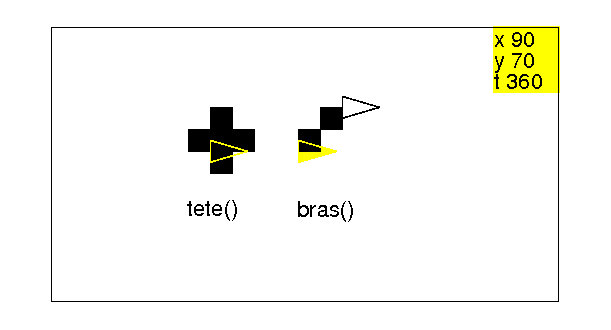
\includegraphics[width=\textwidth]{tortbras}\\
On tape
\begin{verbatim}
tete():={
rectangle_plein;
repete(4,saute,rectangle_plein,tourne_gauche);
}:;
\end{verbatim}

% Generated by xcas tete.tex
%\input figtortue/tete.tex

On d\'efinit la proc\'edure {\tt bras} en tapant :
\begin{verbatim}
bras():={
rectangle_plein ;
saute ;
pas_de_cote ;
rectangle_plein ;
saute ;
pas_de_cote ;
}:;
\end{verbatim}
% Generated by xcas bras.tex
%\input figtortue/bras.tex
Puis on tape :\\
\begin{verbatim}
bonhomme():={
bras();
tourne_droite ;
rectangle_plein 30;
tourne_gauche ;
saute ;
pas_de_cote ;
tete();
pas_de_cote -40;
tourne_gauche 180;
rectangle_plein(10,30);
recule 20;
rectangle_plein(10,30);
pas_de_cote -30;
tourne_gauche ;
bras();
tourne_gauche ;
}:;
\end{verbatim}
Ensuite on peut faire des variantes en r\'ealisant des bonhommes avec les deux 
bras lev\'es ou avec un bras lev\'e et l'autre baiss\'e...puis faire une 
ribambelle. 
On tape par exemple {\tt bonhomme1} qui a le bras gauche baiss\'e et le  bras 
droit lev\'e et {\tt bonhomme2} qui a le bras gauche lev\'e et le  bras 
droit baiss\'e :\\
On tape :
\begin{verbatim}
bonhomme1():={
bras();
tourne_droite ;
rectangle_plein 30;
tourne_gauche ;
saute ;
pas_de_cote ;
tete();
pas_de_cote -40;
tourne_gauche 180;
rectangle_plein(10,30);
recule 20;
rectangle_plein(10,30);
pas_de_cote -20;
tourne_gauche 180;
bras();
tourne_droite ;
}:;
bonhomme2():={
bras();
recule ;
rectangle_plein 30;
tourne_gauche ;
saute ;
pas_de_cote ;
tete();
pas_de_cote -40;
tourne_gauche 180;
rectangle_plein(10,30);
recule 20;
rectangle_plein(10,30);
pas_de_cote -30;
tourne_gauche ;
bras();
tourne_gauche ;
}:;
\end{verbatim}
On tape :
\begin{verbatim}
efface ;
bonhomme1();
crayon rouge;
bonhomme2();
crayon vert;
bonhomme1();
cache_tortue;
\end{verbatim}
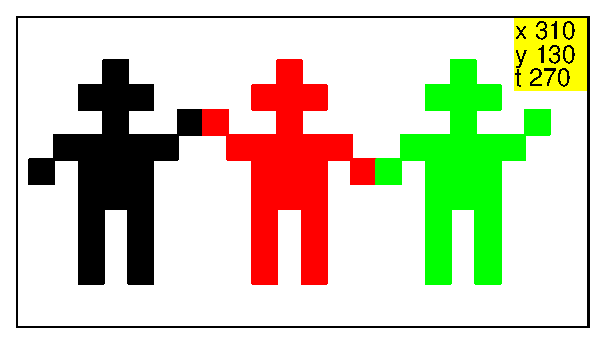
\includegraphics[width=\textwidth]{tortribam}
\section{La maison et le bateau}
Ici on utilise les commandes {\tt rectangle\_plein} ou {\tt triangle\_plein} 
qui dessine un rectangle plein ou un triangle plein, 
\`a gauche de la position de d\'epart de la tortue, la tortue \'etant 
dirig\'ee au d\'epart selon un c\^ot\'e.\\
Voici les dessins du toit, de la maison et du bateau sur lesquels on a not\'e 
\`a l'aide d'un triangle plein la position de d\'epart de la tortue et
 par un triangle la position d'arriv\'ee de la tortue, lorsqu'on ne voit qu'un 
triangle plein c'est que la position d'arriv\'ee de la tortue est la m\^eme 
que sa position de d\'epart.\\
On remarquera que le bateau et la maison se font avec la m\^eme proc\'edure.\\
% Generated by xcas bateau.tex
%\input figtortue/bateau.tex
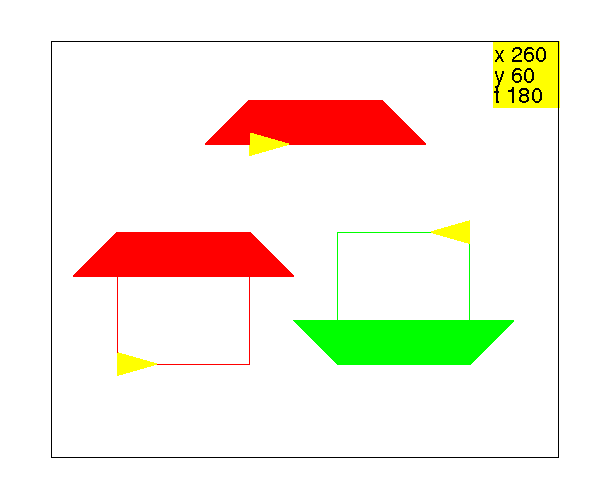
\includegraphics[width=\textwidth]{tortbat}
\begin{verbatim}
toit():={
rectangle_plein(60,20);
tourne_gauche;
triangle_plein(20,20);
pas_de_cote -60;
tourne_droite;
triangle_plein(20,20);
}:;
\end{verbatim}
\begin{verbatim}
maison():={
tourne_gauche;
avance 40;
tourne_droite;
toit();
tourne_droite;
avance 40;
tourne_droite;
avance 60;
tourne_droite 180;
}:;
\end{verbatim}
On tape :\\
{\tt maison()}\\
Ou on tape  :\\
{\tt tourne\_droite 180;bateau()}
\section{Le toit et deux autres bateaux}
Voici les dessins des bateaux que l'on veut r\'ealiser :\\
% Generated by xcas bateaux.tex
%\input figtortue/bateaux.tex
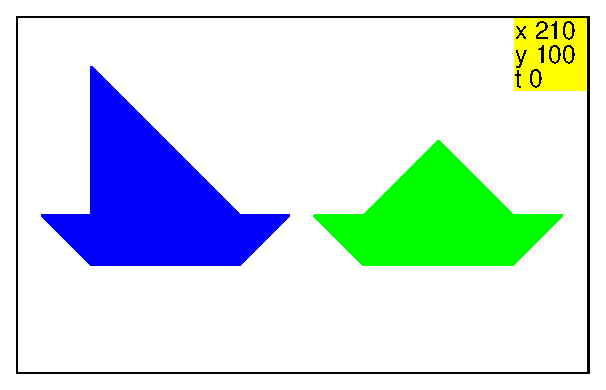
\includegraphics[width=\textwidth]{tortbateau}\\
Il s'agit de r\'eutiliser la proc\'edure {\tt toit} cr\'eer pr\'ec\'edemment.\\
Pour cela on tape, par exemple les proc\'edure {\tt bateau1} et {\tt bateau2} 
dans lesquelles la position d'arriv\'ee de la tortue est aussi sa position de 
d\'epart :
\begin{verbatim}
bateau1():={
tourne_droite 180;
toit();
tourne_droite 180;
triangle_plein(60,60);
saute 60;
}:;
bateau2():={
tourne_droite 180;
toit();
tourne_droite 180;
avance 30;
triangle_plein(30,30);
tourne_gauche;
triangle_plein(30,30);
tourne_droite;
saute 30;
}:;
\end{verbatim}
Puis on demande de faire une frise faite de 2 lignes compos\'ees chacune de 
trois {\tt bateau2}, on veut obtenir :\\
% Generated by xcas frise.tex
%\input figtortue/frise.tex
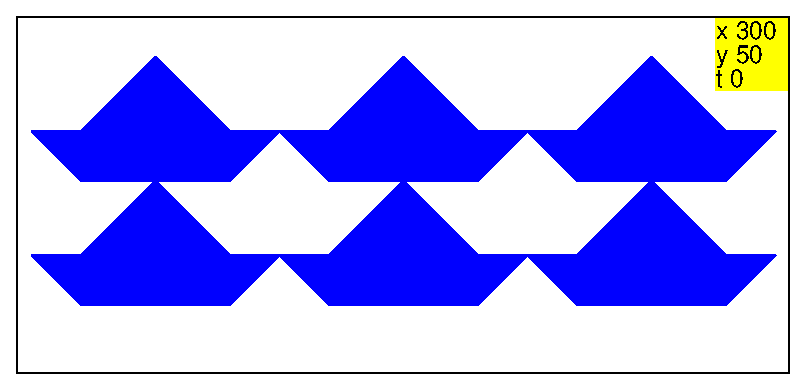
\includegraphics[width=\textwidth]{tortbatfr}\\
On remarque alors qu'il apparait un troisi\`eme bateau que l'on demande de 
d\'efinir.\\
On tape par exemple :
\begin{verbatim}
bateau3():={
tourne_droite;
triangle_plein(30,30);
tourne_droite;
rectangle_plein(40,30);
saute 40;
triangle_plein(30,30);
tourne_droite 180;
saute 20;
triangle_plein(20,20);
tourne_gauche;
triangle_plein(20,20);
tourne_droite ;
saute 20;
}:;
\end{verbatim}
\section{Cr\'eer un pavage}
Comment faire pour que le bateau qui apparait soit le m\^eme ?\\
Autrement trouver un pavage fait avec un seul bateau.\\
Pour avoir un pavage, il faut que les voiles aient la m\^eme 
dimensions que les triangles formant les bords de la coque. Les voiles peuvent 
alors \^etre plac\'ees n'importe o\`u sur la coque. 
On peut donc d\'efinir une proc\'edure param\'etr\'ee avec {\tt n} 
({\tt 0<n<60}) qui sera la place des voiles sur la coque.\\
Par exemple, on tape si on veut encore utiliser {\tt toit} :
\begin{verbatim} 
navire(n):={
tourne_droite 180;
toit();
tourne_droite 180;
saute n;
triangle_plein(20,20);
tourne_gauche;
triangle_plein(20,20);
tourne_droite;
saute 60-n;
}:;
\end{verbatim}
Voici par exemple {\tt navire(10)} et {\tt navire(50)} :\\
% Generated by xcas navire.tex
%\input figtortue/navire.tex
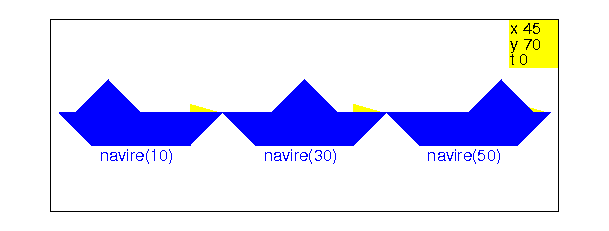
\includegraphics[width=\textwidth]{tortnavs}\\
Voici par exemple un pavage r\'ealis\'e avec {\tt navire(30)} :\\
% Generated by xcas navire30.tex
%\input figtortue/navire30.tex
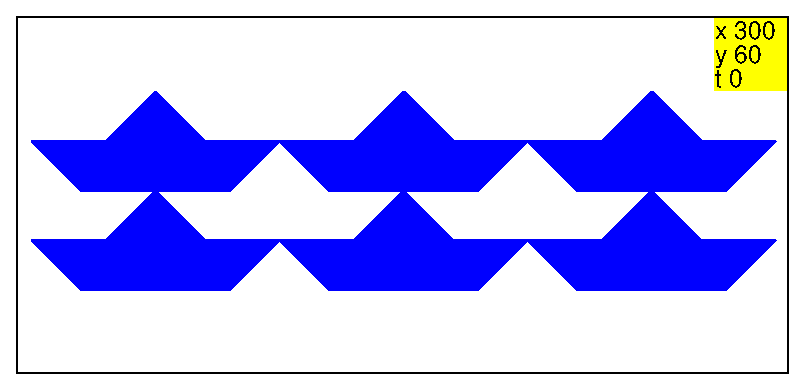
\includegraphics[width=\textwidth]{tortnav}\\
Voici par exemple un pavage r\'ealis\'e avec {\tt navire(10)} :\\
% Generated by xcas navire10.tex
%\input figtortue/navire10.tex
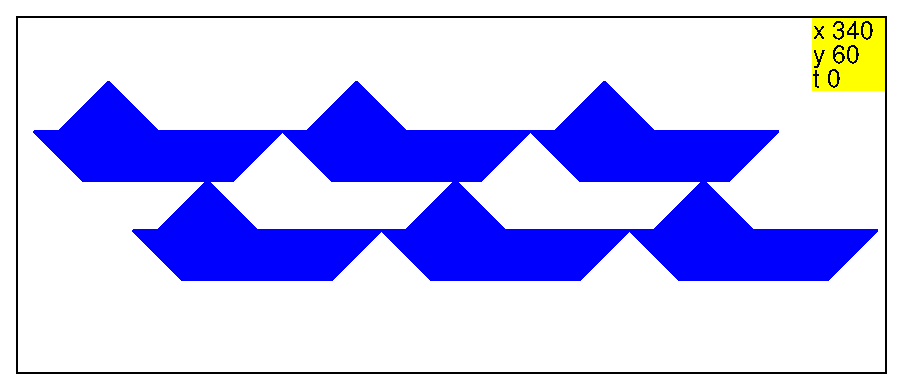
\includegraphics[width=\textwidth]{tortnavf}
ou un pavage  r\'ealis\'e avec {\tt navire(10)} et {\tt navire(50)} :\\
 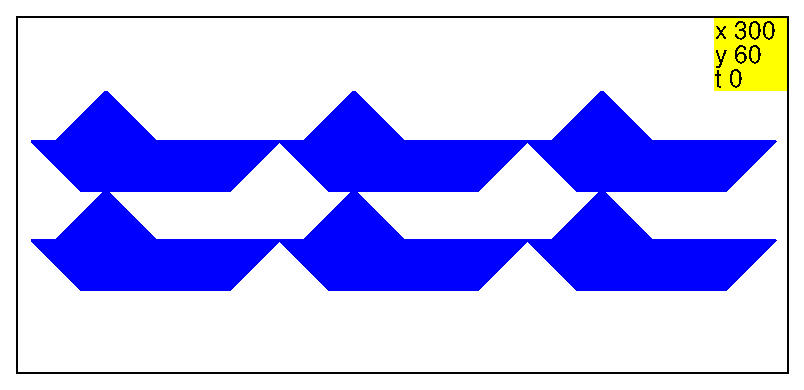
\includegraphics[width=\textwidth]{tortnavfr}\\
Et encore un pavage fait avec les {\tt navire(n)} pour {\tt n=10,20...60}, 
pour cela on tape :
\begin{verbatim}
pavage():={
repete(2,navire(10),saute 100);
navire(10);
saute -240;
pas_de_cote -20;
crayon rouge;
repete(3,navire(20),saute 100);
navire(20);
saute -250;
pas_de_cote -20;
crayon vert;
repete(2,navire(30),saute 100);
navire(30);
saute -260;
pas_de_cote -20;
crayon bleu;
repete(3,navire(40),saute 100);
navire(40);
saute -270;
pas_de_cote -20;
crayon jaune;
repete(2,navire(50),saute 100);
navire(50);
saute -180;
pas_de_cote -20;
crayon magenta;
repete(2,navire(60),saute 100);
navire(60);
saute -230;
pas_de_cote -20;
crayon noir;
repete(3,navire(10),saute 100);
navire(10);
saute -340;
pas_de_cote -20;
crayon rouge;
repete(3,navire(20),saute 100);
navire(20);
saute -250;
pas_de_cote -20;
crayon vert;
repete(2,navire(30),saute 100);
navire(30);
saute -260;
pas_de_cote -20;
crayon bleu;
repete(3,navire(40),saute 100);
navire(40);
saute -270;
pas_de_cote -20;
crayon jaune;
repete(2,navire(50),saute 100);
navire(50);
}:;
\end{verbatim}
Puis on tape :
\begin{verbatim}
efface;
pavage();
cache_tortue;
\end{verbatim}
On obtient :\\
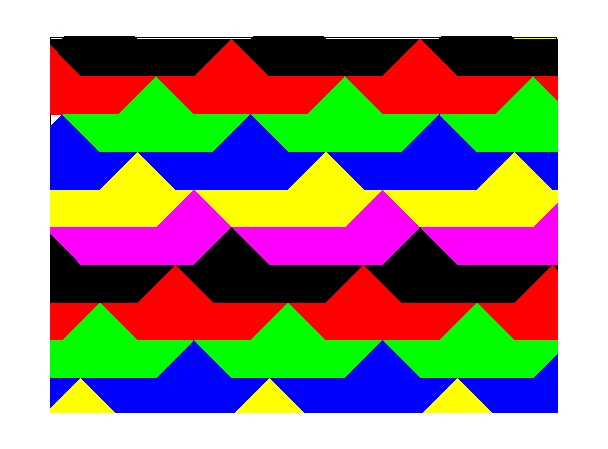
\includegraphics[width=\textwidth]{tortpav}
\section{Cr\'eer une frise avec toit}
On peut faire une ligne compos\'ee de {\tt toit} espac\'ee par {\tt n} pas,
pour cela on tape :
\begin{verbatim}
toit():={
rectangle_plein(60,20);
tourne_gauche;
triangle_plein(20,20);
pas_de_cote -60;
tourne_droite;
triangle_plein(20,20);
};
toits(n):={
repete(3,toit(),saute 40+n);
}:;
\end{verbatim} 
En effet dans la proc\'edure {\tt toit} la tortue a avanc\'e de 60 pas et comme
la longueur du toit est de 100 pas, il faut faire 40 pas, pour r\'ealiser
 un deuxi\`eme toit qui touche le premier.\\
En faisant plusieurs lignes de {\tt toits(0)}, en quinconce, et
n faisant plusieurs lignes de {\tt toits(60)}, on tape :
\begin{verbatim}
efface ;
saute 60;
crayon rouge;
toits(0);
pas_de_cote -20;
saute -350;
crayon vert;
toit();
saute 40;
toits(0);
pas_de_cote -20;
saute -350;
crayon rouge;
toits(0);
saute -60;
pas_de_cote -40;
saute -350;
crayon bleu;
toits(60);
pas_de_cote -20;
saute -400;
crayon jaune;
toits(60);
pas_de_cote -20;
saute -560;
crayon bleu;
toits(60);
cache_tortue;

\end{verbatim}
On obtient :\\
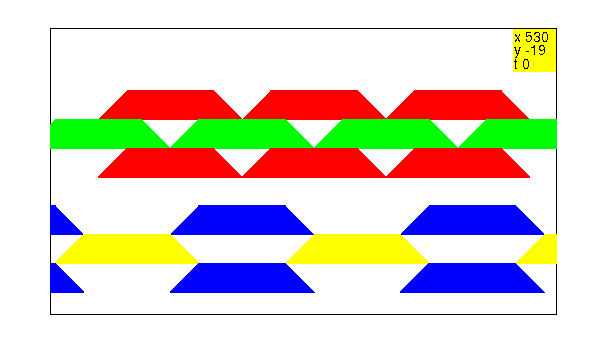
\includegraphics[width=\textwidth]{torttoit}\\
% Generated by xcas toits.tex
%\input figtortue/toits.tex

%En faisant plusieurs lignes de {\tt toits(60)}, en quinconce, on obtient :\\
% Generated by xcas toits60.tex
%\input figtortue/toits60.tex

\section{Le bonhomme de neige et son balai}
Ici on utilise les commandes {\tt disque} ou {\tt rond} qui dessine un disque
ou un cercle \`a partir d'une position de la tortue qui est tangentielle au 
disque ou au cercle.\\
Voici le dessin du bonhomme de neige et de son balai que l'on fera dessiner 
sur papier millim\'etr\'e aux enfants :
le corps est un cercle qui a comme rayon 60, la t\^ete est un cercle qui a
 comme rayon 20, les boutons et les yeux sont des cercles de rayon 6 et
 le chapeau un demi-disque de rayon 10.\\
On choisit comme mod\'ele de balai le dessin ci-dessous sur lequel on a 
mis un petit triangle plein pour d\'esigner le choix de la position de d\'epart
et d'arriv\'ee de la tortue :\\
% Generated by xcas neige.tex
%\input figtortue/neige.tex
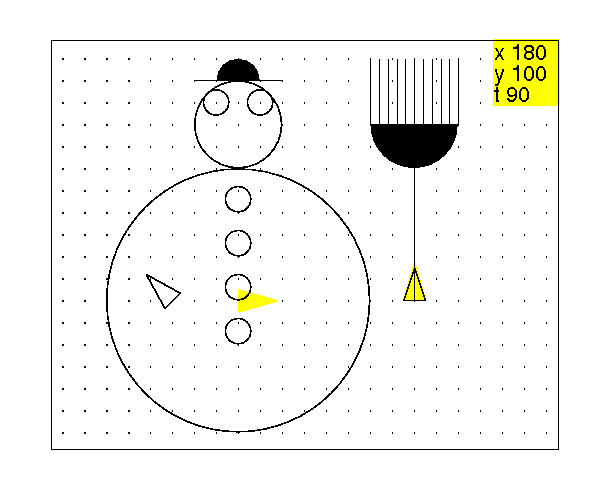
\includegraphics[width=\textwidth]{tortneige}

Si on choisit de prendre comme position de d\'epart 
de la tortue, le centre du corps, avec le cap 0, et une arriv\'ee d\'ecal\'ee 
\`a gauche de 30 pas, par rapport \`a ce centre, et de cap 135 (pour \^etre en position pour mettre le balai),
 On tape :
\begin{verbatim}
bonhomme():={
pas_de_cote 60;
rond 20;
rond -60;
pas_de_cote -20;
rond 6;
pas_de_cote -20;
rond 6;
pas_de_cote -20;
rond 6;
pas_de_cote -20;
rond 6;
pas_de_cote 110;
saute 16;
tourne_gauche;
rond 6;
pas_de_cote 20;
rond 6;
pas_de_cote -4;
saute;
tourne_gauche;
avance 20;
recule 40;
avance;
tourne_droite ;
disque(10,180);
saute 100;
pas_de_cote -20;
tourne_droite 135;
}:;
\end{verbatim}

% Generated by xcas balai.tex
%\input figtortue/balai.tex

On tape :
\begin{verbatim}
balai():={
avance 80;
tourne_gauche;
avance 20;
tourne_gauche;
disque(20,180);
repete(5,avance 30,pas_de_cote 4,recule 30,pas_de_cote 4);
avance 30;
recule 30;
pas_de_cote -20;
recule 80;
} :;
\end{verbatim}
Puis on tape :\\
{\tt bonhomme()}\\
{\tt balai()}\\
On obtient :\\
% Generated by xcas balneige.tex
%\input figtortue/balneige.tex
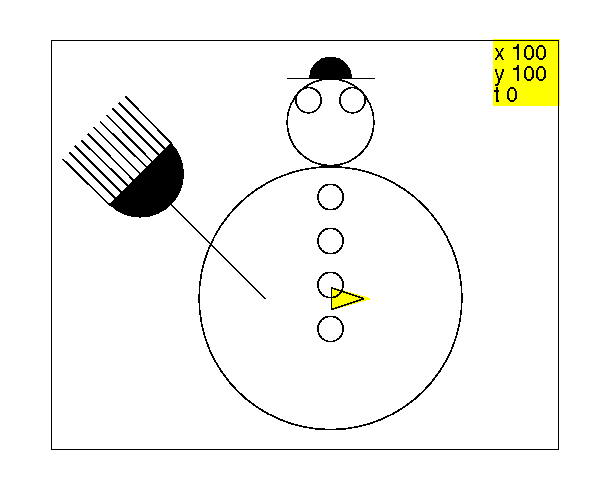
\includegraphics[width=\textwidth]{tortbbn}
\chapter{D'autres exemples d'activit\'es}
\section{Le plan de la classe}
Travail sur le rep\'erage dans le plan et les coordonn\'ees et sur la notion 
d'echelle.\\
Chaque \'el\`eve est responsable du trac\'e de son bureau.\\
Le professeur \'etant charg\'e de tracer son bureau et de d\'eterminer 
par exemple l'empacement des fen\^etres.
\section{La croix de pharmacie}
Faire le trac\'e d'une croix ayant la forme d'un plus.\\
Faire le trac\'e du contour externe d'une croix de pharmacie (les branches 
externes de la croix sont des carr\'es).\\
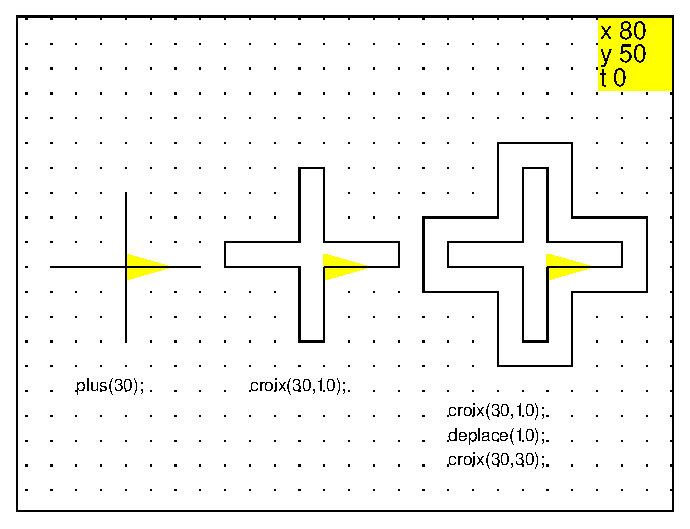
\includegraphics[width=\textwidth]{tortcroix}

Faire le trac\'e de 4 croix emboit\'ees \`a l'image des croix de pharmacie.\\
-Analyse d'un dessin en le d\'ecomposant en \'el\'ements pertinents.\\
-Essayer d'avoir une \'ecriture consise.\\
-Premi\`ere approche de la notion de param\`etres.\\
-Premi\`ere approche de la notion de boucle {\tt pour}.
\begin{verbatim}
plus(a):={
repete(4,avance(a),recule(a),tourne_gauche);
}:;
\end{verbatim}
\begin{verbatim}
croix(a,b):={
repete(4,avance(a),tourne_gauche,avance(b),tourne_gauche,avance(a),tourne_droite);
}:;
\end{verbatim}
\begin{verbatim}
deplace(b):={
saute(b);pas_de_cote(-b);
}:;
\end{verbatim}
Puis, on veut de plus que la position d'arriv\'ee de la tortue soit la m\^eme 
que celle de d\'epart, on tape :
\begin{verbatim}
plus(60);
deplace(10);
croix(60,20);
deplace(10);
croix(60,40);
deplace(10);
croix(60,60);
deplace(-30);
\end{verbatim}
Puis on d\'efinit :
\begin{verbatim}
croix_pharma(a):={
plus(a);
deplace(a/6);
croix(a,a/3);
deplace(a/6);
croix(a,2*a/3);
deplace(a/6);
croix(a,a);
deplace(-a/2);
}:;
\end{verbatim}
On remarque que {\tt plus(a)} fait le m\^eme dessin que {\tt croix(a,0)}, 
l'\'ecriture de la proc\'edure {\tt plus} est donc inutile.
On veut de plus que la position d'arriv\'ee de la tortue soit la m\^eme que 
celle de d\'epart et on veut utiliser une boucle {\tt pour}, on tape :
\begin{verbatim}
croix_pharmacie(a):={
pour n de 0 jusque 3 faire croix(a,n*a/3);deplace(a/6);fpour;
deplace(-2*a/3);
}:;
\end{verbatim}
On peut aussi \'ecrire une proc\'edure r\'ecursive, mais on a alors besion de 2
 param\`etres {\tt a,b} : cette proc\'edure ne dessine rien si {\tt a<b} 
et dessine les croix emboit\'ees avec 10 pas d'\'ecart jusqu'\`a  obtenir la 
{\tt croix(a,a)}.\\
On tape :
\begin{verbatim}
croix_pharmar(a,b):={
si b<=a alors
croix(a,b);
deplace(10);
croix_pharmar(a,b+20);
deplace(-10);
fsi;
}:;
\end{verbatim}
puis on tape :\\
{\tt croix\_pharma(40);saute 130;}
{\tt croix\_pharmar(40,0);}
On obtient :\\
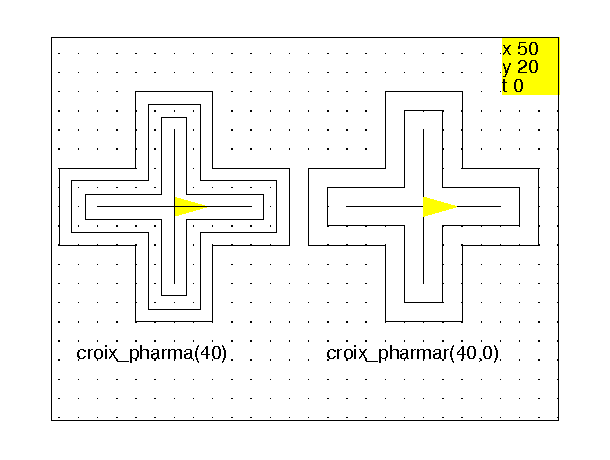
\includegraphics[width=\textwidth]{tortpharma}
\section{Les polygones r\'eguliers}
Faire le trac\'e d'un triangle \'equilat\`eral, d'un carr\'e, d'un hexagone,
 d'un octogone puis, d'un pentagone et d'un polygone r\'egulier ayant 
$n$ cot\'es.\\
\'Ecrire la proc\'edure des triangles \'equilat\`eraux de cot\'es de longueur 
$a$ puis, celle  des carr\'es de cot\'es de longueur $a$ etc...\\
\'Ecrire la proc\'edure des polygones r\'eguliers ayant $n$ cot\'es de longueur
 $a$.\\
Le triangle \'equilat\`eral :
\begin{verbatim}
triequi(a):={
repete(3,avance(a),tourne_gauche(120));
}
\end{verbatim}
Le carr\'e :
\begin{verbatim}
ca(a):={
repete(4,avance(a),tourne_gauche);
}
\end{verbatim}
L'hexagone :
\begin{verbatim}
hexa(a):={
repete(6,avance(a),tourne_gauche(60));
}
\end{verbatim}
L'octogone :
\begin{verbatim}
octo(a):={
repete(8,avance(a),tourne_gauche(45));
}
\end{verbatim}
Le polygone r\'egulier \`a $n$ cot\'es :
\begin{verbatim}
polyg(a,n):={
repete(n,avance(a),tourne_gauche(360/n));
}:;
\end{verbatim}

\section{Les toiles d'araign\'ees}
L'activit\'e consiste \`a tracer des polygones r\'eguliers emboit\'es et de 
dessiner aussi les segments joignant le centre aux sommets du polygone 
ext\'erieur. Cela met en \'evidence le centre du polygone. Mais sans notion de 
trigonom\'etrie c'est difficile. On peut faire faire une toile d'araign\'ee 
hexagonale ou aussi faire cherher par tatonement la longueur de la diagonale
d'un polyg\^one r\'egulier ayant un nombre pair de c\^ot\'es

\subsection{Les toiles d'araign\'ees hexagonales}
On commence par \'ecrire une proc\'edure qui trace un hexagone  de c\^ot\'e 
{\tt l} lorsque la tortue part du centre et est dirig\'ee vers un sommet et 
revient  \`a son point de d\'epart.\\
On tape :
\begin{verbatim}
hexag_centre(l):={
avance l;
tourne_gauche 120;
repete(6,avance l,tourne_gauche 60);
tourne_droite 120;
recule l;
}:;
\end{verbatim}
On dessine les diagonales de l'hexagone centr\'e facilement, on tape :
\begin{verbatim}
diag_hexagc(l):={
repete(6,avance l,recule l,tourne_gauche 60);
}:;
\end{verbatim} 
Pour faire la toile il faut faire des hexagones emboit\'es avec un pas de 
{\tt p}. On dessine les hexagones de c\^ot\'es {\tt p, 2p,3p...} et on donne le 
nombre {\tt n} d'hexagones. La tortue part du centre de la toile, est dirig\'ee
selon un sommet de la toile et revient \`a son point de d\'epart.\\
On tape :
\begin{verbatim}
araign6(p,n):={
diag_hexagc(n*p);
pour j de 1 jusque n faire 
hexag_centre(j*p);
fpour;
}:;  
\end{verbatim} 
On peut remarquer qu'il n'est pas astucieux de faire revenir la tortue au 
centre lorsqu'on a fait un hexagone et que ce serait mieux de passer au suivant
directement. On \'ecrit alors la proc\'edure {\tt hexag} qui dessine un 
hexagone direct de c\^ot\'e {\tt l} lorsque la tortue part d'un sommet et est 
dirig\'ee selon un c\^ot\'e.\\
On tape :
\begin{verbatim}
hexag(l):={
repete(6,avance l,tourne_gauche 60);
}:;
\end{verbatim}
La toile est obtenue en tapant (la tortue part du centre et revient au centre) :
On tape :
\begin{verbatim}
toile6(p,n):={
diag_hexagc(n*p);
pour j de 1 jusque n faire 
avance p;
tourne_gauche 120;
hexag(j*p);
tourne_droite 120;
fpour;
recule n*p;
}:;
\end{verbatim}
On tape ;\\
{\tt efface ;araign6(10,7);}\\
Ou on tape :\\
{\tt efface ;toile6(10,7);}\\
On obtient :\\
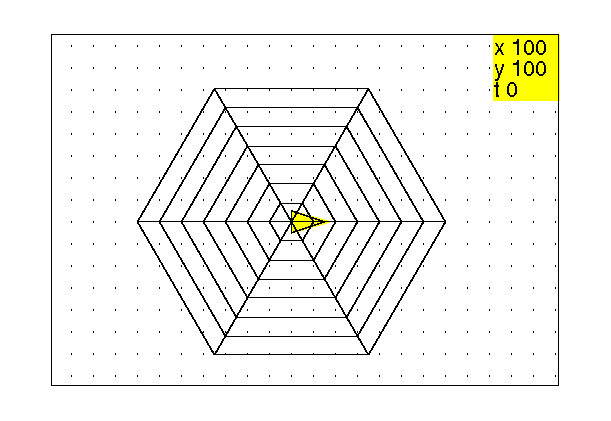
\includegraphics[width=\textwidth]{tortaraign}

\subsection{Une activit\'e sur la proportionalit\'e}
On essaye par essai et erreur de trouver la longueur de la diagonale d'un
octogone.\\
On tape :
\begin{verbatim}
octog(l):={
repete(8,avance l,tourne_gauche 45);
}:;
\end{verbatim}
Puis, on tape :
\begin{verbatim}
efface ;
crayon jaune;
dessine_tortue;
crayon noir;
octog(80);
tourne_gauche 135/2;
avance 200;
\end{verbatim}
On obtient :\\
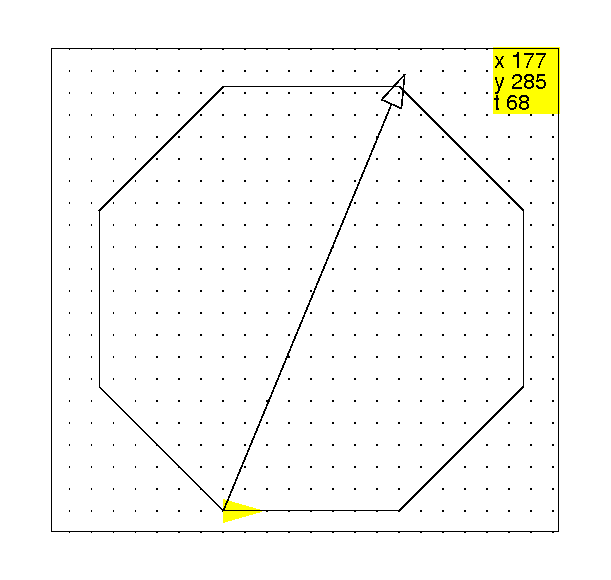
\includegraphics[width=\textwidth]{tortoctog}\\
Puis on fait des essais et on estime que la dagonale vaut d'un octogone de 
c\^ot\'e 80 vaut 209.\\
On remplit le tableau suivant en faisantt calculer par {\tt Xcas} la derni\`ere
ligne avec {\tt Digits:=4} :\\
\begin{tabular}{|l|r|r|r|r|r|r|r|}
\hline
$cote$&40&50&60&70&80&90&100\\
\hline
$diagonale$&&&&&&&\\
\hline
$\frac{diagonale}{cote}$& & & & & & & \\
\hline
\end{tabular}

On obtient par exemple :\\
\begin{tabular}{|l|r|r|r|r|r|r|r|}
\hline
$cote$&40&50&60&70&80&90&100\\
\hline
$diagonale$&104.5&130.5&157.&183.&209.&235.&261.\\
\hline
$\frac{diagonale}{cote}$&2.612&2.61&2.617&2.614&2.612&2.611&2.61\\
\hline
\end{tabular}

On en d\'eduit que :\\
$diagonale*cote\simeq 2.61$.\\
\begin{verbatim}
toile8(p,n):={
repete(8,avance n*p*2.61/2,recule n*p*2.61/2,tourne_gauche 45);
pour j de 1 jusque n faire 
avance p*2.61/2;
tourne_gauche 135/2+45;
octog(j*p);
tourne_droite 135/2+45;
fpour;
recule n*p*2.61/2;
}:;
\end{verbatim}
Puis, on tape :
\begin{verbatim}
efface ;
crayon jaune;
dessine_tortue;
crayon noir;
toile8(10,5);
\end{verbatim}
On obtient :
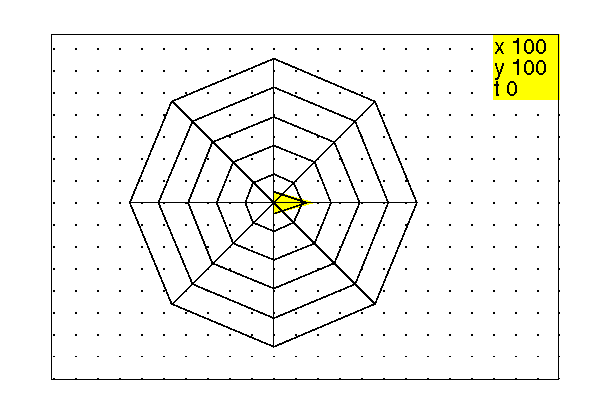
\includegraphics[width=\textwidth]{tortaraign8}
\subsection{La toile d'araign\'ee et la trigonom\'etrie}
On \'ecrit une proc\'edure qui trace un polygone r\'egulier direct de {\tt k} 
c\^ot\'es de longueur {\tt l} lorsque la tortue part d'un sommet et est 
dirig\'ee vers un sommet et revient  \`a son point de d\'epart.\\
On tape :
\begin{verbatim}
polyg(l,k):={
repete(k,avance l,tourne_gauche 360/k);
}:;
\end{verbatim}
La proc\'edure {\tt araignee(k,p,n)} trace  
{\tt n} polygones emboit\'es, r\'eguliers, directs et de {\tt k} 
c\^ot\'es o\`u le plus petit polygone $P$ a des c\^ot\'es de longueur {\tt p}. 
La distance du centre de $P$ a un de ces sommets donne l'espacement entre les 
diff\'erents polygones. La tortue part du centre et est 
dirig\'ee vers un sommet et revient \`a son point de d\'epart.
On tape dans l'\`editeur de programme :
On tape :
\begin{verbatim}
araignee(k,p,n):={
local r,j;
r:=p/sin(pi/k)/2;
repete(k,avance n*r,recule n*r,tourne_gauche 360/k);
pour j de 1 jusque n faire 
saute r;
tourne_gauche 90+180/k;
crayon rouge;
polyg(j*p,k);
tourne_droite 90+180/k;
fpour;
saute -n*r;
}:;
\end{verbatim}
Puis, on tape :
\begin{verbatim}
efface ;
crayon jaune;
dessine_tortue;
crayon noir;
araignee(9,10,8);
\end{verbatim}
On obtient :\\
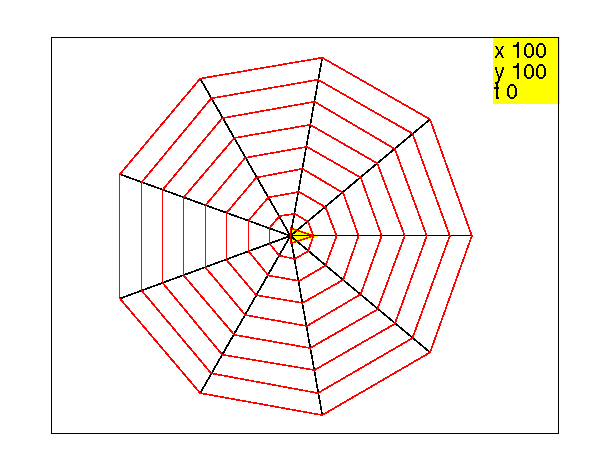
\includegraphics[width=\textwidth]{tortaraigne}
On peut \'ecrire une proc\'edure r\'ecursive :
\begin{verbatim}
araigneer(k,p,n):={
local r;
r:=p/sin(pi/k)/2;
crayon noir;
repete(k,avance n*r,recule n*r,tourne_gauche 360/k);
si n>0 alors 
saute n*r;
tourne_gauche 90+180/k;
crayon rouge;
polyg(n*p,k);
tourne_droite 90+180/k;
saute -n*r;
araigneer(k,p,n-1)
fsi;}
:;
\end{verbatim}
\section{Le drapeau anglais}
L'activit\'e consiste \`a tracer un carr\'e avec ses diagonales et ses 
m\'edianes.\\
Au d\'ebut, les dimensions du carr\'e ne sont pas impos\'ees.\\
On fait ensuite varier le cot\'e du carr\'e.
Cette activit\'e est double :\\
-travail sur les valeurs approch\'ees (quelle est la longueur de la diagonale 
d'un carr\'e ?),\\
-travail sur les proc\'edures param\'etr\'ees.\\
On choisit de faire partir la tortue en bas et \`a gauche du drapeau, on tape :
\begin{verbatim}
drapeau(a):={
repete(4,avance(a),tourne_gauche);
leve_crayon;
avance(a/2);tourne_gauche;avance(a/2);
baisse_crayon;
repete(4,avance(a/2),saute(-a/2),tourne_gauche);
tourne_gauche(45);
repete(4,avance(a*sqrt(2)/2),saute(-a*sqrt(2)/2),tourne_gauche);
tourne_droite(45);
leve_crayon;
recule(a/2);tourne_droite;recule(a/2);
baisse_crayon;
}:;
\end{verbatim}
Ou encore, on choisit de faire partir la tortue au centre du drapeau, on tape :
\begin{verbatim}
carre_diag(a):={
repete(4,avance(a),tourne_gauche);
tourne_gauche(45);
avance(a*sqrt(2));
saute(-a*sqrt(2));
tourne_droite(45);
}:;
\end{verbatim}
\begin{verbatim}
drapeau_centre(a):={
repete(4,carre_diag(a/2),tourne_gauche);
}:;
\end{verbatim}
On tape :\\
{\tt drapeau(80);saute 160;}
{\tt pas\_de\_cote 40;}
{\tt drapeau\_centre(80);}
On obtient :\\
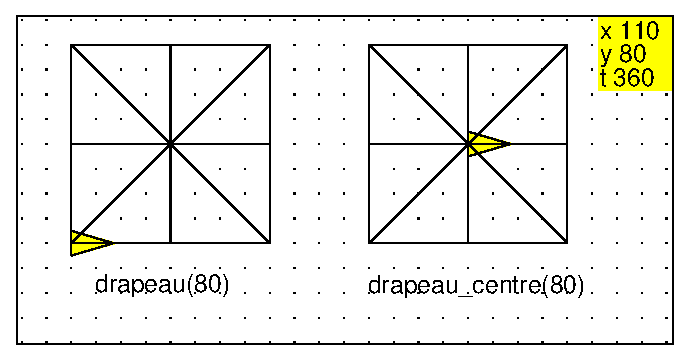
\includegraphics[width=\textwidth]{tortdrap}

ou encore
\begin{verbatim}
triang(a):={
repete(2,avance(a),tourne_gauche);
avance(a);
saute(-a);
tourne_gauche(45);
avance(a*sqrt(2));
tourne_gauche(135);
}:;
\end{verbatim}
\begin{verbatim}
drapeaut(a):={
repete(4,triang(a/2),tourne_gauche);
}:;
\end{verbatim}

\section{La famille des sapins et la proportionali\'e}
{\bf 1-i\`ere s\'eance}\\
On dessine un triangle rectangle isoc\`ele plein et direct $ABC$ avec comme 
position de d\'epart et d'arriv\'ee de la tortue, le milieu de l'hypot\'enuse 
$BC$ avec un cap dirig\'e selon le vecteur $BC$.
\begin{verbatim}
tri(a):={
triangle_plein(a,a);
tourne_droite;
triangle_plein(a,a);
tourne_gauche;
}:;
\end{verbatim}
On dessine un sapin form\'e de 2 triangles {\tt tri} de dimensions 50 et 40 pas
de tortue et  d\'ecal\'es de 40 pas de tortue, avec comme position de d\'epart 
et d'arriv\'ee de la tortue le milieu de l'hypot\'enuse avex un  cap dirig\'e 
selon la hauteur de {\tt tri(50)}.

% Generated by xcas sapin.tex
%\input figtortue/sapin.tex
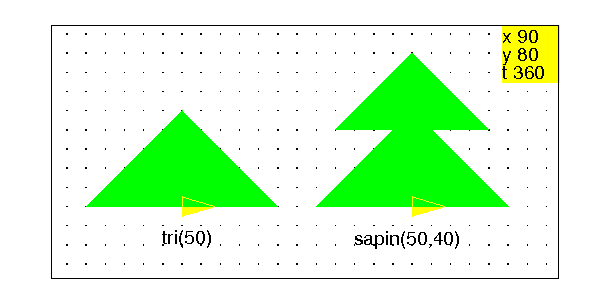
\includegraphics[width=\textwidth]{tortsapin}

Pour faire le dessin dans l'\'ecran de {\tt g\'eom\'etrie} :
\begin{verbatim}
//dessin du triangle qui represente la tortue
tortue_g(a):={
[triangle_rectangle(a,a+0.1,2),triangle_rectangle(a,a+0.2*i,0.5)];
}
//dessin du triangle rectangle isocele d'hypothenuse 2a
tri_g(a,l):={
[triangle_rectangle(a,a+l,1),triangle_rectangle(a,a+i*l,1)];
}
sapin_g(a,l1,l2):={
[triangle_rectangle(a,a+l1,1),triangle_rectangle(a,a+i*l1,1),triangle_rectangle(a+i*l2,a+i*l2+l2,1),triangle_rectangle(a+i*l2,a+2*i*l2,1)];
}
\end{verbatim}
puis 
\begin{verbatim}
tortue_g(-3);
tri_g(-3,1);
legende(-3.5-0.5*(i),"tri(50)");
tortue_g(0);
sapin_g(0,0.8,1);
legende(-0.5-0.5*(i),"sapin(50,40)");
\end{verbatim}

Revenons \`a la tortue, on \'ecrit la proc\'edure {\tt sapin} :
\begin{verbatim}
sapin():={
tri(50);
avance(40);
tri(40);
recule(40);
}:;
\end{verbatim}

{\bf 2-i\`eme s\'eance}\\
On demande d'\'ecrire \`a partir de sapin une proc\'edure param\'etr\'ee avec 
2 param\`etres {\tt a}  et {\tt b} : {\tt a} pour {\tt 50} et {\tt b} pour 
{\tt 40}.\\
On \'ecrit en classe en expliquant : 
\begin{verbatim}
sapin(a,b):={
tri(a);
avance(b);
tri(b);
recule(b);
}
\end{verbatim}
On a donc fait dessiner la derni\`ere fois {\tt sapin(50,40)}.\\
On demande maintenant de dessiner les sapins de la famille du   
{\tt sapin(50,40)},
c'est \`a dire ceux qui ont la m\^eme forme 
que lui \`a un agrandissement ou \`a une r\'educion pr\`es.\\
On demande aux enfants de remplir le tableau suivant :\\
\begin{tabular}{|l|l|}
\hline
a &b\\
\hline
5& \\
10& \\
15& \\
20& \\
25& \\
30& \\
35& \\
40& \\
45& \\
50&40 \\
55& \\
60& \\
70& \\
80& \\
90& \\
100& \\
\hline
\end{tabular}

Les enfants remplissent tous le tableau au d\'ebut en se servant 
syst\'ematiquement de l'addition ils \'ecrivent :\\
\begin{tabular}{|l|l|}
\hline
a &b\\
\hline
15& 5\\
20& 10\\
25& 15\\
30& 20\\
35& 25\\
40& 30\\
45& 35\\
50& 40 \\
\hline
\end{tabular}

Mais lorsqu'il testent {\tt sapin(20,10)} ils n'obtiennent qu'un seul triangle
et s'apercoivent que'il y a une erreur....et ils sont alors oblig\'es de 
proc\'eder par essais et erreurs ...mais cela est quelquefois difficile car il
n'y a gu\'ere de diff\'erence entre {\tt sapin(45,35)} et {\tt sapin(45,36)}.\\
Il faut donc demander :\\
si {\tt a=100} que vaut {\tt b} ?\\
si {\tt a=25} que vaut {\tt b} ?\\
si {\tt a=5} que vaut {\tt b} ?\\
si {\tt a=10} que vaut {\tt b} ?\\
si {\tt a=20} que vaut {\tt b} ?\\
Comment \'ecrire cette famille avec un seul param\`etre ?
On veut arriver  \`a l'\'ecriture de la proc\'edure :
\begin{verbatim}
famille_sapin(k):={
sapin(5*k,4*k);
}
\end{verbatim}
Ainsi le {\tt sapin(50,40)} est le m\^eme que {\tt famille\_sapin(10)}.

\section{La sym\'etrie orthogonale}
Activit\'e r\'ealis\'ee dans une classe de CM2.\\
Les \'el\`eves viennent de faire des travaux pratiques de physique sur la r\'eflexion de la lumi\`ere : fabrication de p\'eriscope, boite noire et image r\'efl\'echie par un miroir.\\
Ils ont observ\'e comment un dessin trac\'e sur une feuille de papier se 
r\'efl\'echit dans un miroir, lorsqu'on pose ce miroir perpendiculairement \`a 
cette feuille.\\
Les sym\'etriques de dessins faits sur un tableau noir muni d'un quadrillage
sont r\'ealis\'es ais\'ement lorsque la droite symbolisant le miroir est
une horizontale ou une verticale ou encore est inclin\'ee de 45 ou de 135
 degr\'es en passant par des n{\oe}ud du quadrillage, mais le quadrillage est 
source d'erreur quand  le sym\'etrique d'un n{\oe}ud n'est pas un n{\oe}ud.
\subsection{Premi\`ere s\'eance en informatique}
Je dessine au tableau les dessins suivants :\\
un drapeau, un k\'epi, une casserole :\\
%kepi.tex
%\input figtortue/kepi.tex
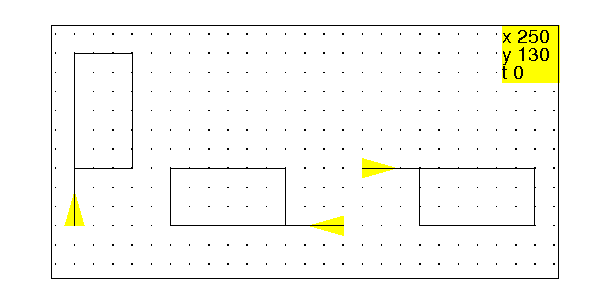
\includegraphics[width=\textwidth]{tortkepi}\\
Il faut que les enfants fasse dessiner \`a la tortue :
\begin{itemize}
\item le miroir qui doit avoir une position quelconque,
\item un des objets ci-dessus : l'objet doit avoir une position quelconque par
 rapport au miroir,
\item l'image de l'objet  cr\'ee par le miroir. 
\end{itemize}
Voici ce que font la plupart des enfants :
le trac\'e d'une droite {\tt D} horizontale ou verticale puis le trac\'e d'un 
drapeau et de son sym\'etrique. Il donne un nom \`a cette suite d'instruction par exemple {\tt exercice}. Puis pour r\'epondre \`a la consigne :\\
le miroir doit avoir une position quelconque, il tape :\\
{\tt efface; tourne\_droite(30);exercice} 
\subsection{Deuxi\`eme s\'eance en informatique}
On demande de d\'efinir une fonction {\tt objet} qui dessine un objet avec au 
plus 5 traits. Puis on demande de refaire le m\^eme travail que lors de la 
premi\`ere s\'eance en dessinant le sym\'etrique de {\tt objet} par rapport 
\`a $D$  mais la position de {\tt objet} par rapport \`a la droite ne doit pas
 \^etre fig\'ee.\\
Il faut donc pr\'evoir une fonction {\tt place\_objet}
qui place l'objet par rapport \`a la droite ainsi qu'une fonction 
{\tt place\_objetsym} qui place l'objet sym\'etrique par 
rapport \`a la droite et une fonction {\tt objetsym} qui dessine le
 sym\'etrique de {\tt objet}.
\begin{verbatim}
axe(c):={
pas_de_cote(100);
tourne_gauche(c);
avance(200);
recule(400);
avance(200);
};
objet():={
avance 30;
repete(2,avance 60,tourne_droite,avance 30,tourne_droite);
recule 30;
};
objetsym():={
avance(30);
repete(2,avance(60),tourne_gauche,avance(30),tourne_gauche);
recule(30);
};
place_objet(a,b):={
leve_crayon;
tourne_gauche;
avance a;
tourne_gauche b;
baisse_crayon;
};
replace_tortue(a,b):={
leve_crayon;
tourne_droite b;
recule a;
tourne_droite;
baisse_crayon;
};
place_objetsym(a,b):={
leve_crayon;
tourne_droite;
avance a;
tourne_droite b;
baisse_crayon;
};
retoursym(a,b):={
leve_crayon;
tourne_gauche b;
recule a;
tourne_gauche;
baisse_crayon;
};
exo(a,b,c):={
efface;
axe(c);
place_objet(a,b);
objet();
replace_tortue(a,b);
place_objetsym(a,b);
objetsym();
retoursym(a,b);
tourne_droite c;
pas_de_cote(-100);
};
\end{verbatim}
Puis on tape : {\tt exo(30,40,20)}

\section{Feuille de TP}
Voici la feuille d'un TP suivi d'une correction possible o\`u l'on a utilis\'e 
{\tt pas\_de\_cote}.
\begin{center}{\bf La tortue et la sym\'etrie orthogonale par rapport \`a une droite}\end{center}
\subsection{Exercice I}
Voici les dessins d'un drapeau, d'un k\'epi, d'une casserole :\\
%\input figtortue/kepi.tex
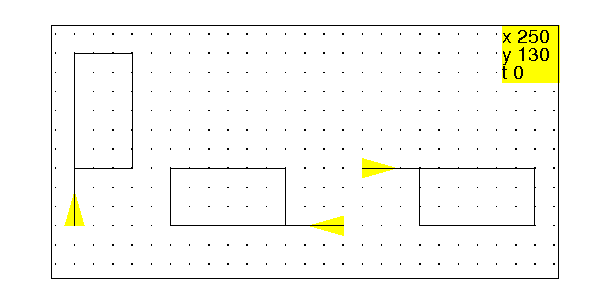
\includegraphics[width=\textwidth]{tortkepi}\\
1/ \'Ecrire une proc\'edure {\tt objet} qui r\'ealise l'un de ces dessins : on 
prendra soin de noter sur le dessin la position choisie pour
le d\'epart et l'arriv\'ee de la tortue.

2/ On veut dessiner l'image de {\tt objet} dans un miroir, pour cela :
\begin{itemize}
\item Dessiner une droite qui symbolise un miroir : le miroir doit avoir une position quelconque,
\item Dessiner l'objet ci-dessus : l'objet doit avoir une position quelconque 
par rapport au miroir,
\item Dessiner l'image de l'objet  cr\'ee par le miroir. 
\end{itemize}

\subsection{Exercice II}
1/ Refaire l'exercice pr\'ec\'edent en \'ecrivant les proc\'edures suivantes :
\begin{itemize}
\item {\tt miroir} qui trace une droite, 
\item {\tt place\_miroir} qui place et oriente le miroir,
\item {\tt objet} qui dessine l'objet de votre choix, 
\item {\tt place\_objet} qui place et oriente l'objet par rapport au miroir,
%\item {\tt replace\_tortue} qui replace et r\'eoriente la tortue selon sa position avant d'avoir fait {\tt place\_objet}
\item {\tt objetsym} qui dessine l'objet sym\'etrique par rapport au miroir,
\item {\tt place\_objetsym} qui place et oriente {\tt objetsym} selon le
 sym\'etrique de {\tt objet} par rapport au miroir,
\end{itemize}
2/ Comment peut-on \'ecrire de fa\c{c}on automatique la proc\'edure 
{\tt objetsym} \`a partir de la proc\'edure {\tt objet} ?\\
Comment peut-on \'ecrire de fa\c{c}on automatique la proc\'edure 
{\tt place\_objetsym} \`a partir de la proc\'edure {\tt place\_objet} ?
\subsection{Corrections}
Une solution pour l'exercice I peut \^etre :
\begin{verbatim}
objet(a):={
avance(a);
repete(2,avance(2*a),tourne_droite,avance(a),tourne_droite);
recule(a);
};
objetsym(a):={
avance(a);
repete(2,avance(2*a),tourne_gauche,avance(a),tourne_gauche);
recule(a);
};
exo1():={
pas_de_cote(200);
objet(40);
pas_de_cote(-100);
tourne_droite(20);
avance(200);
recule(400);
avance(200);
tourne_droite(110);
saute(100);
tourne_gauche;
objetsym(40);
}
\end{verbatim}
Les proc\'edures de l'exercice II :
\begin{verbatim}
miroir():={
avance(200);
recule(400);
avance(200);
};
place_miroir(d):={
pas_de_cote(100);
tourne_gauche(d);
miroir();
}
\end{verbatim}
Le param\`etre {\tt d} repr\'esente l'angle du miroir avec l'horizontale.\\
Le param\`etre {\tt b} repr\'esente la distance du d\'epart de l'objet avec le 
miroir et le param\`etre {\tt c} repr\'esente son inclinaison par rapport au 
miroir.
\begin{verbatim}
place_objet(b,c):={
pas_de_cote(-b);
tourne_gauche(c);
};
replace_tortue(b,c):={
tourne_droite(c);
pas_de_cote(b);
};
place_objetsym(b,c):={
pas_de_cote(b);
tourne_droite(c);
}
\end{verbatim}
On remarque que la proc\'edure {\tt place\_objetsym} est inutile puisque :\\
{\tt place\_objetsym(b,c)=place\_objet(-b,-c)}.\\
\`A la fin pour remettre la tortue sur le miroir on utilisera
{\tt replace\_tortue(-b,-c)}
On peut aussi \'ecrire la proc\'edure {\tt objet2} qui r\'ealise 
{\tt objet} (resp {\tt objetsym}) quand la valeur du deuxi\`eme param\`etre 
est 1 (resp -1).
\begin{verbatim}
objet2(a,s):={
avance(a);
repete(2,avance(2*a),tourne_droite s*90,avance(a),
       tourne_droite s*90);
recule(a);
}
\end{verbatim}
et alors 
{\tt objet(a):=objet2(a,1)}
 et {\tt objetsym(a):=objet2(a,-1)}

On \'ecrit alors :
\begin{verbatim}
exo2(a,b,c,d):={
place_miroir(d);
miroir();
place_objet(b,c);
objet(a);
replace_tortue(b,c);
place_objetsym(b,c)
objetsym(a);
replace_tortue(-b,-c);
}
\end{verbatim}
ou encore, si on suppose que le miroir est dessin\'e et que la tortue est sur 
le miroir, on peut utiliser la proc\'edure suivante :
\begin{verbatim}
finexo2(a,b,c):={
place_objet(b,c);
objet2(a,1);
replace_tortue(b,c);
place_objet(-b,-c)
objet2(a,-1);
replace_tortue(-b,-c);
};
exo2(a,b,c,d):={
place_miroir(d);
miroir();
finexo2(a,b,c);
}
\end{verbatim}
On tape par exemple :\\
{\tt exo2(40,100,20,-10)}
{\tt finexo2(-20,40,30)}
{\tt finexo2(...)}
\chapter{Pour avoir un fond quadrill\'e ou triangul\'e}
\section{Fond quadrill\'e}
On fait une proc\'edure {\tt maillage1(a,k)} qui trace avec la couleur {\tt k}
un \'ecran remplit de car\'es de c\^ot\'es {\tt a}.
\subsection{Le programme}
\begin{verbatim}
//a represente la longueur du carreau et k la couleur du maillage
maillage1(a,k):={
local p,c,cc;
p:= position;
c:=cap;
cc:=crayon;
leve_crayon;position([0,0]);cap 0;baisse_crayon;crayon k;
repete(ceil(260/a),avance(ceil(400/a)*a),pas_de_cote(a),
tourne_droite 180, avance(ceil(400/a)*a),pas_de_cote(-a),
tourne_droite 180);
leve_crayon;position([0,0]);cap 0;baisse_crayon;
tourne_gauche; 
repete(ceil(200/a),avance(ceil(520/a)*a),pas_de_cote(-a),
tourne_droite 180, avance(ceil(520/a)*a),pas_de_cote(a),
tourne_droite 180);
crayon(cc);
leve_crayon;position(p);
cap(c);baisse_crayon;
}
\end{verbatim}
\subsection{Utilisation}
On tape :\\
{\tt maillage1(30,22)}\\
On obtient un fond quadrill\'e avec des carr\'es de c\^ot\'es 30 de couleur 
gris p\^ale de code 22.

\section{Fond triangul\'e}
On fait une proc\'edure {\tt maillage2(a,k)} qui trace avec la couleur {\tt k}
un \'ecran form\'e d'un maillage dont les mailles sont des triangles 
\'equilat\'eraux de c\^ot\'es {\tt a}.
\subsection{Le programme}
\begin{verbatim}
//a represente la longueur du triangle et k la couleur du maillage
//tricot fait un zig-zag a droite ou a gauche selon que s=-1 ou 1
tricot(a,s):={
repete(ceil(400/a),avance a,tourne_gauche s*120,avance a,
tourne_droite s*120)
};
maillage2(a,k):={
local p,c,cc;
p:= position;
c:=cap;
cc:=crayon;
leve_crayon;position([0,0]);cap 0;baisse_crayon;crayon k;
repete(ceil(200/a),avance(ceil(400/a)*a),tourne_gauche 120,
tricot(a,1),avance a,tourne_droite 120,avance(ceil(400/a)*a),
tourne_droite 120,avance -a,tricot(a,-1),tourne_gauche 120);
crayon(cc);
leve_crayon;position(p);
cap(c);baisse_crayon;
}
\end{verbatim}
\subsection{Utilisation}
On tape :\\
{\tt maillage2(30,22)}\\
On obtient un fond triangul\'e avec des triangles \'equilat\'eraux de c\^ot\'es
30 et de couleur gris p\^ale de code 22.

\chapter{La recursivit\'e sur des exemples}
\section{Des spirales}
\subsection{Une spirale}
Voici le d\'ebut du dessin d'une spirale(90) :\\
%\input figtortue/spirale.tex
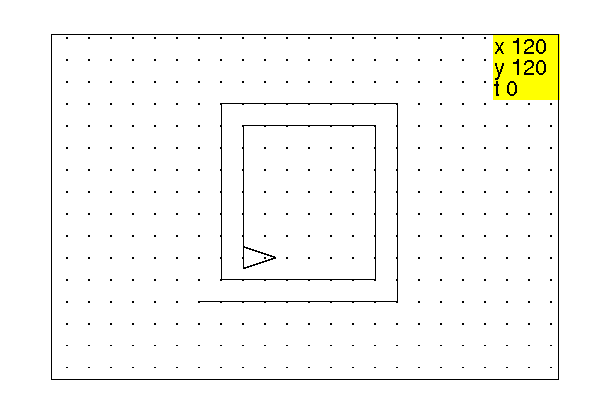
\includegraphics[width=\textwidth]{tortspi}\\
On tape dans un \'editeur de programmes :
\begin{verbatim}
spirale(l):={
si (l>10) alors 
avance(l);
tourne_gauche 90;
avance(l);
tourne_gauche 90;
spirale(l-10);
fsi;
}
\end{verbatim}
On tape dans une ligne de commande :\\
{\tt efface;spirale(100)}\\
On obtient :\\
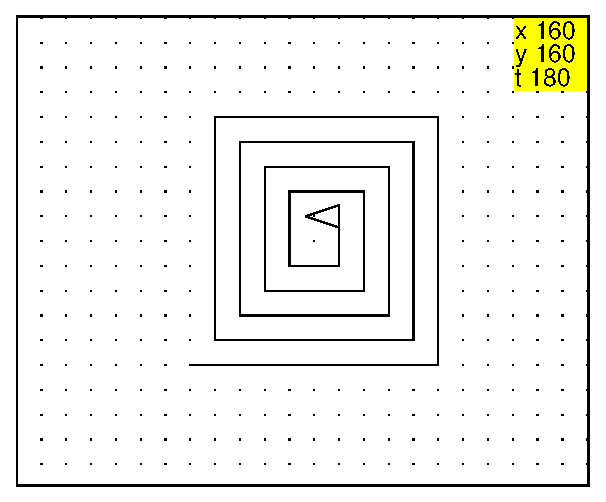
\includegraphics[width=\textwidth]{tortspir}
\subsection{Une spirale plus g\'en\'erale}
On tape dans un \'editeur de programmes :
\begin{verbatim}
//chaque segment de la spirale est obtenu par similitude de rapport k 
//k=rapport et t=angle de rotation (externe)
//n=nombre de segments a construire
spirales(l,k,t,n):={
pour j de 1 jusque n faire
avance(l);
tourne_gauche(t);
l:=k*l;
fpour;
};
\end{verbatim}
ou encore avec la recursivit\'e
\begin{verbatim}
//n=nombre de segments a construire=nombre d'appels recursifs
spiraler(l,k,t,n):={
si n>0 alors
 avance(l);
 tourne_gauche(t);
 spiraler(l*k,k,t,n-1);
fsi;
}:;
\end{verbatim} 
On tape par exemple dans une ligne de commande :\\
{\tt spirales(90,0.8,60,20)}\\
ou\\
{\tt efface;spiraler(90,0.8,60,20)}\\
On obtient :\\
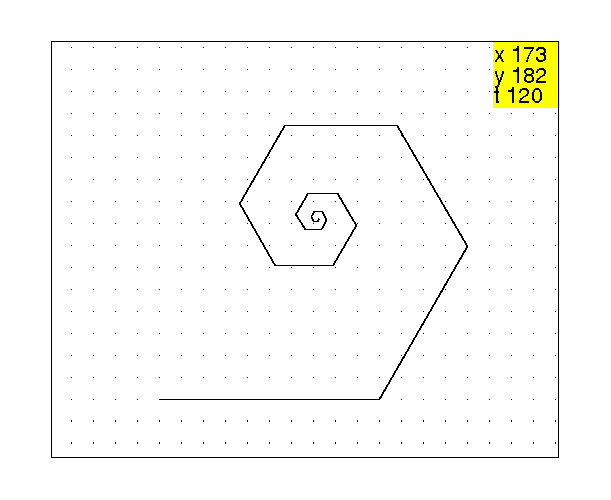
\includegraphics[width=\textwidth]{tortspirr}
%\input figtortue/spiraler.tex

\section{Des arbres}
\subsection{Un arbre a deux branches}
Un arbre est compos\'e d'un tronc de hauteur $h$ et de deux branches 
sym\'etriques faisant 45 degr\'es avec le tronc et que l'on d\'efinit comme 
\'etant chacune un arbre de tronc $h/2$.\\
Pour le r\'ealiser, on tape dans un \'editeur de programmes : 
\begin{verbatim}
//tourne_gauche;arbre1(60)
arbre1(h):={
si (h<5) alors
avance(h);
recule(h);
sinon
avance(h);
tourne_droite(45);
arbre1(h/2);
tourne_gauche(90);
arbre1(h/2):
tourne_droite(45);
recule(h);
fsi;
}:;
\end{verbatim}
On valide avec {\tt OK} ou avec {\tt F9}.\\
On tape par exemple dans une ligne de commande :\\
{\tt efface;tourne\_gauche;arbre1(60)}\\
On obtient :\\
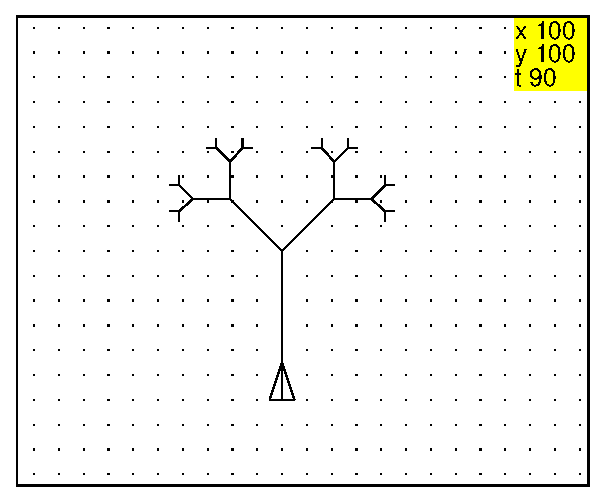
\includegraphics[width=\textwidth]{tortarb1}\\
Ou bien, on rajoute un param\`etre $n$ (la profondeur) pour faire le test 
d'arr\^et, on tape on tape dans un \'editeur de programmes : 
\begin{verbatim}
//tourne_gauche;arbre2(60,3)
arbre2(h,n):={
si (n==0) alors
avance(h);
recule(h);
sinon
avance(h);
tourne_droite(45);
arbre2(h/2,n-1);
tourne_gauche(90);
arbre2(h/2,n-1):
tourne_droite(45);
recule(h);
fsi;
}:;
\end{verbatim}
On valide avec {\tt OK} ou avec {\tt F9}.\\
On tape par exemple dans une ligne de commande :\\
{\tt efface;tourne\_gauche;arbre2(60,5)}\\
On obtient :\\
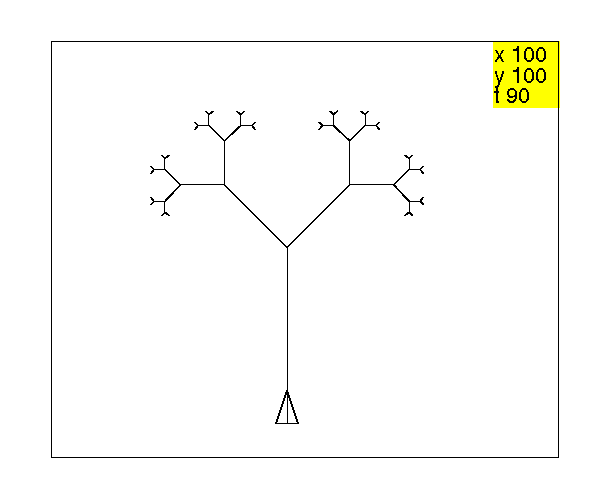
\includegraphics[width=\textwidth]{tortarb2}\\
\subsection{Un arbre a $p$ branches}
Un arbre est compos\'e d'un tronc de hauteur $h$ et de $p$ branches 
\'egalement r\'eparties et que l'on d\'efinit comme 
\'etant chacune un arbre de tronc $h/2$.\\
On tape dans un \'editeur de programmes :
\begin{verbatim}
//tourne_gauche;arbre3(80,4)
arbre3(h,p):={
si (h<5) alors
avance(h);
recule(h);
sinon
avance(h);
tourne_droite(90*(p-1)/p);
repete(p,arbre3(h/2,p),tourne_gauche(180/p));
tourne_droite(90*(p+1)/p);
recule(h);
fsi;
}:;
\end{verbatim}
On valide avec {\tt OK} ou avec {\tt F9}.\\
On tape par exemple dans une ligne de commande :\\
{\tt efface;tourne\_gauche;arbre3(80,4)}\\
On obtient :\\
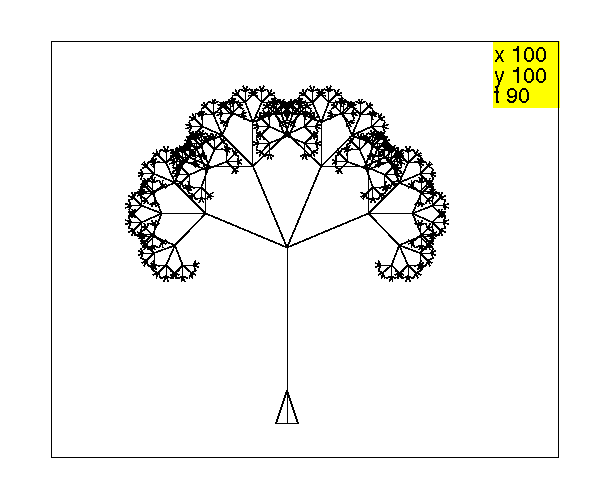
\includegraphics[width=\textwidth]{tortarb3}\\
Ou bien, on rajoute un param\`etre $n$ (la profondeur) pour faire le test 
d'arr\^et, on tape dans un \'editeur de programmes :
\begin{verbatim}
//tourne_gauche;arbre4(60,5,3)
arbre4(h,p,n):={
si (n==0) alors
avance(h);
recule(h);
sinon
avance(h);
tourne_droite(90*(p-1)/p);
repete(p,arbre4(h/2,p,n-1),tourne_gauche(180/p));
tourne_droite(90*(p+1)/p);
recule(h);
fsi;
}:;
\end{verbatim}
On valide avec {\tt OK} ou avec {\tt F9}.\\
On tape par exemple dans une ligne de commande :\\
{\tt efface;tourne\_gauche;arbre4(80,5,4)}\\
On obtient :\\
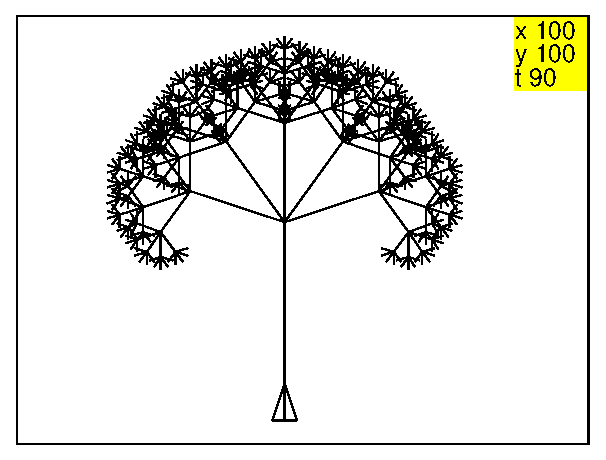
\includegraphics[width=\textwidth]{tortarb4}\\


Et maintenant, un arbre al\'eatoire : \\
\`a chaque n{\oe}ud on choisit, de fa\c{c}on al\'eatoire le rapport $k$ de 
r\'eduction, qui fera les $p$ branches comme un arbre r\'eduit avec le 
coefficient $k$.\\
On tape dans un \'editeur de programmes :
\begin{verbatim}
//tourne_gauche ;saute(-80);arbre5(60,4,3);
arbre5(h,p,n):={
local k;
si (n==0) alors
avance(h);
recule(h);
sinon
avance(h);
tourne_droite(90*(p-1)/p);
k:=hasard(0,1);
repete(p,arbre5(h*k,p,n-1),tourne_gauche(180/p));
tourne_droite(90*(p+1)/p);
recule(h);
fsi;
}:;
\end{verbatim}
On valide avec {\tt OK} ou avec {\tt F9}.\\
On tape par exemple dans une ligne de commande :\\
{\tt efface;tourne\_gauche;arbre5(60,5,4)}\\
On obtient :\\
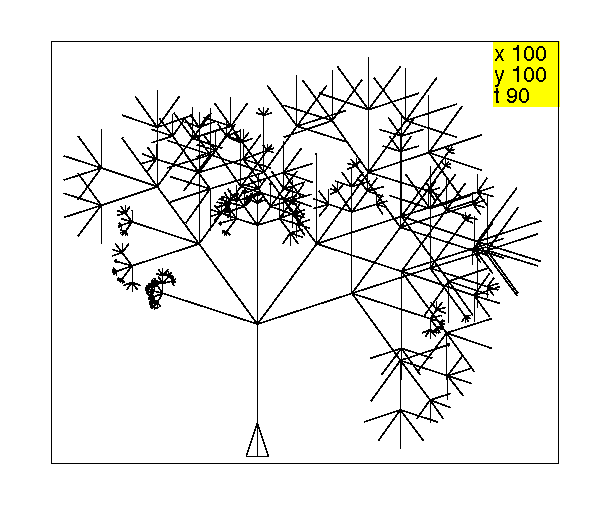
\includegraphics[width=\textwidth]{tortarb5}\\


Et enfin, un arbre encore plus al\'eatoire : \\
pour chaque branche on choisit, de fa\c{c}on al\'eatoire le rapport 
{\tt hasard(0,1)} de r\'eduction, qui fera cette branche comme un arbre 
r\'eduit avec ce coefficient.\\
On tape dans un \'editeur de programmes :
\begin{verbatim}
//tourne_gauche ;saute(-80);arbre6(60,4,3);
arbre6(h,p,n):={
si (n==0) alors
avance(h);
recule(h);
sinon
avance(h);
tourne_droite(90*(p-1)/p);
repete(p,arbre6(h*hasard(0,1),p,n-1),tourne_gauche(180/p));
tourne_droite(90*(p+1)/p);
recule(h);
fsi;
}:;
\end{verbatim}
On valide avec {\tt OK} ou avec {\tt F9}.\\
On tape par exemple dans une ligne de commande :\\
{\tt efface;tourne\_gauche;arbre6(60,5,4)}\\
On obtient :\\
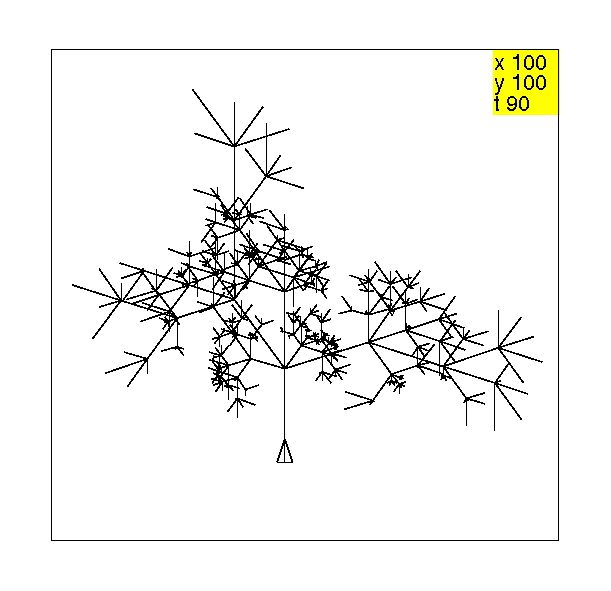
\includegraphics[width=\textwidth]{tortarb6}\\


\subsection{Un arbre ramifi\'e}
Ici on suppose que, du tronc de longueur $h$,
 il part $p$ branches de longueur $h/2$.
Ces branches donnent naissance \`a $p-1$ branches de longueur $h/4$ etc...
jusqu'\`a $p=2$.
On tape dans un \'editeur de programmes :
\begin{verbatim}
//tourne_gauche;saute(-80);arbre7(60,5)
arbre7(h,p):={
avance(h);
si (p>=2) alors
tourne_droite(90*(p-1)/p);
repete(p,arbre7(h/2,p-1),tourne_gauche(180/p));
tourne_droite(90*(p+1)/p);
fsi;
recule(h);
}:;
\end{verbatim}
On valide avec {\tt OK} ou avec {\tt F9}.\\
On tape par exemple dans une ligne de commande :\\
{\tt efface;tourne\_gauche;arbre7(80,5)}\\
On obtient :\\
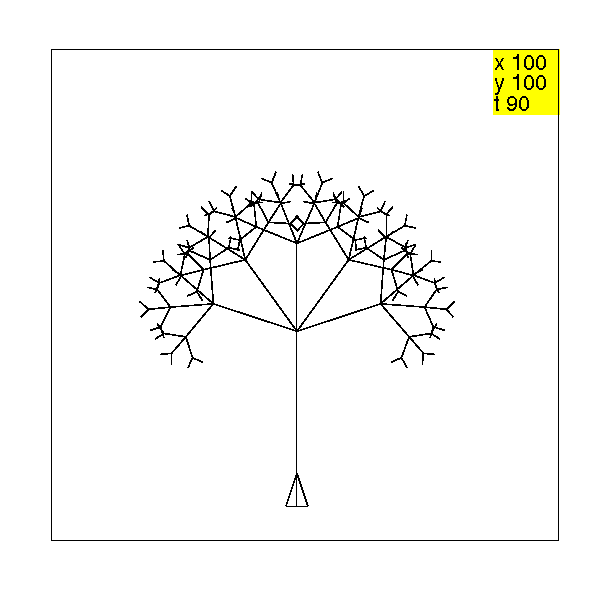
\includegraphics[width=\textwidth]{tortarb7}\\

%On obtient :
%\input figtortue/arbrera.tex

En utilisant aussi la profondeur dans le test d'arr\^et on tape dans un 
\'editeur de programmes :
\begin{verbatim}
//tourne_gauche;saute(-80);arbre8(90,5,3)
arbre8(h,p,n):={
avance(h);
si (p>=2 et n>=1) alors
tourne_droite(90*(p-1)/p);
repete(p,arbre8(h/2,p-1,n-1),tourne_gauche(180/p));
tourne_droite(90*(p+1)/p);
fsi;
recule(h);
}:;
\end{verbatim}
On valide avec {\tt OK} ou avec {\tt F9}.\\
On tape par exemple dans une ligne de commande :\\
{\tt efface;tourne\_gauche;arbre8(80,6,5)}\\
On obtient :\\
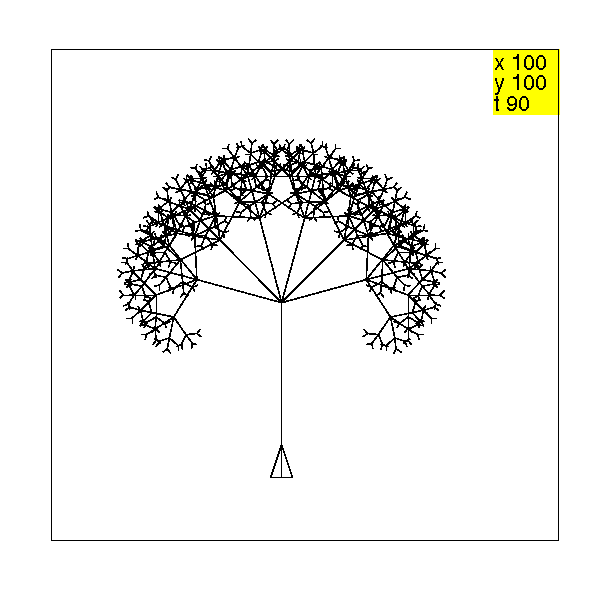
\includegraphics[width=\textwidth]{tortarb8}\\

%Les 8 proc\'edures ci-dessus se trouvent dans le fichier :\\
%{\tt examples/tortue/arbre.cxx}.\\
{\bf Exercice}
Refaire les exemples pr\'ec\'edents mais en ne dessinant que la frondaison de 
l'arbre, c'est \`a dire l'arbre sans son tronc.\\
{\bf Une r\'eponse}
Voici la r\'eponse correspondant \`a {\tt arbre7} et \`a {\tt arbre8}. Bien 
s\^ur, pour avoir la frondaison de {\tt arbre7(60,5)} il faut taper 
{\tt arbre9(30,5)} et pour avoir la frondaison de {\tt arbre8(60,5,3)} il faut 
taper {\tt arbre10(30,5,3)}.
\begin{verbatim}
//tourne_gauche;saute(-80);arbre9(90,5,3)
arbre9(h,p):={
si (p>=2) alors
tourne_droite(90*(p-1)/p);
repete(p,avance(h),arbre9(h/2,p-1),recule(h),tourne_gauche(180/p));
tourne_droite(90*(p+1)/p);
fsi;
}
\end{verbatim}
\begin{verbatim}
//tourne_gauche;saute(-80);arbre10(90,5,3)
arbre10(h,p,n):={
si (n>=1 et p>=2) alors
tourne_droite(90*(p-1)/p);
repete(p,avance(h),arbre10(h/2,p-1,n-1),recule(h),tourne_gauche(180/p));
tourne_droite(90*(p+1)/p);
fsi;
}
\end{verbatim}
\subsection{Un sapin}
Pour d\'ecrire un sapin, il faut choisir un param\`etre par exemple sa hauteur 
$h$ du sapin.\\ 
On dit alors qu'un sapin de hauteur $h$ est compos\'e de :
\begin{itemize}
\item deux branches basses lat\'erales sym\'etriques de longueur $h/2$ et 
faisant un angle de 60 degr\'es avec le tronc,
\item d'un bout de tronc de hauteur $h/4$,
\item d'une t\^ete de hauteur $3h/4h$ .
\end{itemize}
Cette d\'efinition sera r\'ecursive si on dit que les deux branches basses 
lat\'erales sont des sapins plus petits (de hauteur \'egale \`a la  moiti\'e de
 la hauteur du sapin) et que la t\^ete est aussi un  sapin plus petit 
(de hauteur \'egale au trois-quart de la hauteur du sapin). Le tronc a donc 
pour hauteur le quart de  la hauteur du 
sapin. Il nous faut alors d\'efinir ce que l'on consid\'ere 
comme sapin "initial" : c'est le sapin form\'e d'un tronc unique. \\ 
Voici la croissance de ces sapins :\\

%\input figtortue/sapinr.tex
\includegraphics[width=\textwidth]{tortsap}\\

On tape dans un \'editeur de programme :
\begin{verbatim}
//tourne_gauche;sapin1(90)
sapin1(h):={
si (h<5) alors
avance(h);
recule(h);
sinon
tourne_droite(60);
sapin1(h/2);
tourne_gauche(120);
sapin1(h/2):
tourne_droite(60);
avance(h/4);
sapin1(3*h/4);
recule(h/4);
fsi;
}:;
\end{verbatim}
Ou on tape en utilisant pour faire le test d'arr\^et la profondeur $n$ :
\begin{verbatim}
//tourne_gauche;sapin2(90,4)
sapin2(h,n):={
si (n==0) alors
avance(h);
recule(h);
sinon
tourne_droite(60);
sapin2(h/2,n-1);
tourne_gauche(120);
sapin2(h/2,n-1):
tourne_droite(60);
avance(h/4);
sapin2(3*h/4,n-1);
recule(h/4);
fsi;
}:;
\end{verbatim}
On valide avec {\tt OK} ou avec {\tt F9}.\\
On tape par exemple dans une ligne de commande :\\
{\tt efface;tourne\_gauche;sapin2(100,7)}\\
On obtient :\\
\includegraphics[width=\textwidth]{tortsap2}\\
Les diff\'erentes \'etapes ont \'et\'e obtenus en ex\'ecutant :\\
{\tt tourne\_gauche; sapin2(90,0)} puis\\
{\tt tourne\_gauche; sapin2(90,1)} puis\\
{\tt tourne\_gauche; sapin2(90,2)} puis\\
{\tt tourne\_gauche; sapin2(90,3)}.  
%Les 2 proc\'edures ci-dessus se trouvent dans le fichier :\\{\tt examples/tortue/sapin.cxx}

\section{Les flocons de Koch}
Voici les \'etapes de construction d'une courbe 
d\'ecouverte par  Koch :

%\input figtortue/flocon.tex
\includegraphics[width=\textwidth]{tortkoch}\\
On voit l'\'etape 0 : un segment de longueur $l$.\\
Pour obtenir l'\'etape 1, on divise ce segment de longueur $l$ en trois et on 
r\'ealise la deuxi\`eme figure qui est compos\'ee de quatre segments de 
longueur $l/3$ (le deuxi\'eme et troisi\'eme segments sont les c\^ot\'es d'un 
triangle \'equilat\'eral),
puis on recommence en transformant chacun de ces 4 segments en 4 segments....\\
et cela tant que $l \geq 10$.
%La  troisi\'eme figure est alors {\tt koch1(90)}.\\
On tape dans un \'editeur de programme :
\begin{verbatim}
//koch1(90)
koch1(l):={
si (l<10) alors
avance(l);
sinon
koch1(l/3);tourne_gauche(60);
koch1(l/3);tourne_droite(120);
koch1(l/3);tourne_gauche(60);
koch1(l/3);
fsi;
}:;
\end{verbatim}
Ou on tape en utilisant un param\`etre $n$ repr\'esentant la profondeur (i.e. 
le nombre d'appels r\'ecursifs) :
\begin{verbatim}
//koch2(90,3)
koch2(l,n):={
si (n==0) alors
avance(l);
sinon
koch2(l/3,n-1);tourne_gauche(60);
koch2(l/3,n-1);tourne_droite(120);
koch2(l/3,n-1);tourne_gauche(60);
koch2(l/3,n-1);
fsi;
}:;
\end{verbatim}
On valide avec {\tt OK} ou avec {\tt F9}.\\
On tape par exemple dans une ligne de commande :\\
{\tt efface;koch2(270,7)}\\
On obtient :\\
\includegraphics[width=\textwidth]{tortkoch2}\\
Les dessins des diff\'erentes \'etapes ont \'et\'e obtenus en tapant :\\
{\tt koch2(90,0)}  puis, \\
{\tt koch2(90,1)}  puis, \\
{\tt koch2(90,2)} \\
%Les 2 proc\'edures ci-dessus se trouvent dans le fichier :\\{\tt examples/tortue/koch.cxx}

\section{Les courbes de P\'eano}
Parmi les nombreuses courbes invent\'ees par P\'eano, prouvant l'existence de 
courbes remplissant un carr\'e, on n'en retiendra que trois, celles d\'ecrites 
dans les paragraphes suivants.
\subsection{La courbe $\mathcal C^0$ de P\'eano}
Soit un carr\'e de diagonale $l$ :\\
au jour 0, on trace une diagonale,\\
au jour 1, on divise ce carr\'e en 9 carr\'es et on trace les diagonales de ces
 carr\'es, de fa\c{c}on \`a avoir un trait continu en parcourant la premi\`ere 
ligne, puis la deuxi\`eme, et enfin la troisi\`eme, comme ci-dessous :\\
%\input figtortue/peano.tex
\includegraphics[width=\textwidth]{tortpeano}\\

puis on recommence le m\^eme processus.\\
On tape dans un \'editeur de programme :
\begin{verbatim}
//peano(90)
peano(l):={
  si (l<10) alors avance(l);
  sinon
  peano(l/3);
  tourne_droite;peano(l/3);
  tourne_gauche;peano(l/3);
  tourne_gauche;peano(l/3);
  tourne_gauche;peano(l/3);
  tourne_droite;peano(l/3);
  tourne_droite;peano(l/3);
  tourne_droite;peano(l/3);
  tourne_gauche;peano(l/3);
  fsi
}:;
\end{verbatim}
On valide avec {\tt OK} ou avec {\tt F9}.\\
On tape par exemple dans une ligne de commande :\\
{\tt efface;tourne\_gauche 45;peano(200)}\\
On obtient :\\
\includegraphics[width=\textwidth]{tortpeano1}
\subsection{La courbe de P\'eano binaire}
Soit un carr\'e de cot\'e $l$ :\\
au jour 0, on trace un segment de longueur $l$ i.e. un cot\'e du carr\'e,\\
au jour 1, on remplace ce segment, en tra\c{c}ant 4 segments de longueur $l/2$ 
qui sont dispos\'es selon les trois cot\'es d'un rectangle situ\'e \`a gauche 
de la position de la tortue, de largeur $l/2$ et de longueur $l$,\\
au jour 2, on remplace chaque segment de longueur $k$ par 4 segments de 
longueur $k/2$ en tracant les trois 
co\'es d'un rectangle de largeur $k/2$ et de longueur $k$ et situ\'e soit 
\`a droite soit \`a gauche de la position de la tortue comme cela :\\
%\input figtortue/peanobi.tex
\includegraphics[width=\textwidth]{tortpeanob}\\
 puis on recommence le m\^eme processus.\\
On remarque que l'on remplace un segment en tracant un rectangle situ\'e soit 
\`a droite soit \`a gauche de la position de la tortue : on introduit donc un 
param\`etre $s$ qui vaut 1 si ce rectangle se situe \`a droite et qui vaut -1 
si ce rectangle se situe \`a gauche.\\ 
On tape :
\begin{verbatim}
//peanob(90,1)
peanob(l,s):={
  si (l<10) alors avance(l);
  sinon
  tourne_gauche(-90*s);peanob(l/2,-s);
  tourne_droite(-90*s);peanob(l/2,s);
  peanob(l/2,s);tourne_droite(-90*s);
  peanob(l/2,-s);tourne_gauche(-90*s);
  fsi
}:;
\end{verbatim}
On valide avec {\tt OK} ou avec {\tt F9}.\\
On tape par exemple dans une ligne de commande :\\
{\tt efface;peanob(200,-1)}\\
On obtient :\\
\includegraphics[width=\textwidth]{tortpeanob1}

\subsection{La courbe de P\'eano ternaire}
Au jour 1, on trace la premi\`ere courbe {\tt peano1(l,0)} dans le carr\'e de 
cot\'e $l$,\\
Au jour 2, on trace la deux\`eme courbe dans le carr\'e de cot\'e $l$
obtenue en partageant le carr\'e en 9 carr\'es et en tra\c{c}ant dans le premier carr\'e {\tt peano1(l,0)}, et dans les autres soit  
{\tt peano1(l,1)}, soit  {\tt peano1(l,-1)}, de fa\c{c}on \`a ce que les 
courbes se raccordent entre elles.\\
Voici les dessins, o\`u la position de d\'epart et d'arriv\'ee de la tortue est
 choisie comme indiqu\'ee sur la premi\`ere figure :\\
%\input figtortue/peanoter.tex
\includegraphics[width=\textwidth]{tortpeanot}\\
\hspace*{0.5cm}{\tt peano1(60,0)} {\tt peano1(60,1)} {\tt peano1(60,-1)}
On d\'ecide alors de prendre comme d\'epart de la tortue le 
sommet inf\'erieur gauche du carr\'e. On d\'efinit {\tt car(l)} qui dessine un 
carr\'e de c\^ot\'e {\tt l}, on tape :
\begin{verbatim}
//carre de cote l
car(l):={
repete(4,avance(l),tourne_gauche 90);
}:;
//peano1(30,0) ou peano1(30,1) ou peano1(30,-1)
peano1(l,s):={
si (s==-1) alors 
  tourne_droite(45);saute(-l*sqrt(2)/6);rond(round(l*sqrt(2)/6.),90);
sinon 
  si (s==1) alors
   tourne_gauche(135);saute(-l*sqrt(2)/6);rond(round(-l*sqrt(2)/6.),90);
  sinon
   tourne_gauche(45);
   saute(l*sqrt(2)/6);
  fsi;
fsi;
rond(round(l*sqrt(2)/6.),90);
rond(round(-l*sqrt(2)/6.),270);
rond(round(l*sqrt(2)/6.),270);
rond(round(-l*sqrt(2)/6.),90);
saute(l*sqrt(2)/6);
tourne_droite(45);
}:;
//peanot(90,0)
peanot(l,s):={
  si (l<31) alors 
    peano1(l,s);
  sinon
    peanot(l/3,s);
    tourne_droite;peanot(l/3,1);
    tourne_gauche;peanot(l/3,-1);
    tourne_gauche;peanot(l/3,-1);
    tourne_gauche;peanot(l/3,-1);
    tourne_droite;peanot(l/3,1);
    tourne_droite;peanot(l/3,1);
    tourne_droite;peanot(l/3,1);
    tourne_gauche;peanot(l/3,-1);
  fsi;
}:;
\end{verbatim}
On valide avec {\tt OK} ou avec {\tt F9}.\\
On tape par exemple dans une ligne de commande :\\
\begin{verbatim}
dessine_tortue;
crayon jaune;
car(90);
crayon noir;
peanot(90,0);
\end{verbatim}
On obtient :\\
\includegraphics[width=\textwidth]{tortpeanot1}\\
% fltk N4xcas7EditeurE 709 74 231 399 20 0
%fltk N4xcas10Log_OutputE 16 473 924 1 20 0

Mais, on voit qu'\`a cause des erreurs d'arrondis, la courbe n'est pas centr\'ee
dans le carr\'e. En particuler, {\tt peanot(120,0), peanot(110,0),peanot(100,0)}
donne le m\^eme dessin !!!

  On d\'ecide alors de prendre comme d\'epart de la tortue le 
centre du carr\'e.
\begin{verbatim}
carc(l):={
pas_de_cote -l/2;
repete(4,avance l/2,tourne_gauche ,avance l/2);
pas_de_cote l/2;
}:;
pean1(l,s):={
tourne_gauche 45;
rond(round(l*sqrt(2)/6.),270);
rond(round(-l*sqrt(2)/6.),90);
si (s==-1) alors 
  rond(round(-l*sqrt(2)/6.),90);
  tourne_droite 180;
  rond(round(l*sqrt(2)/6.),90);
sinon 
  si (s==1) alors
   rond(round(l*sqrt(2)/6.),90); 
   tourne_droite 180;
   rond(round(-l*sqrt(2)/6.),90);
   sinon tourne_droite 180;
  fsi;
fsi;
rond(round(l*sqrt(2)/6.),90);
rond(round(-l*sqrt(2)/6.),270);
tourne_droite 225;
}:;
pean2(l,s):={
tourne_droite 135;
rond(round(l*sqrt(2)/6.),270);
rond(round(-l*sqrt(2)/6.),90);
tourne_droite 180;
rond(round(l*sqrt(2)/6.),90);
rond(round(-l*sqrt(2)/6.),270);
tourne_gauche -45;
}:;
pean(l,s):={
pean2(l,s);
pean1(l,s)
}:;
peant(l,s):={
  si (l<31) alors 
    pean(l,s);
  sinon
  pas_de_cote -l/3;
  saute -l/3;
  peant(l/3,s);
  saute l/3;tourne_droite;peant(l/3,1);
  pas_de_cote l/3;tourne_gauche;peant(l/3,-1);
  pas_de_cote l/3;tourne_gauche;peant(l/3,-1);
  pas_de_cote l/3;tourne_gauche;peant(l/3,-1);
  saute l/3;tourne_droite;peant(l/3,1);
  saute l/3;tourne_droite;peant(l/3,1);
  saute l/3;tourne_droite;peant(l/3,1);
  pas_de_cote l/3;tourne_gauche;peant(l/3,-1);
  pas_de_cote -l/3;saute -l/3;
fsi;
}:;
\end{verbatim}
On valide avec {\tt OK} ou avec {\tt F9}.\\
On tape par exemple dans une ligne de commande :\\
\begin{verbatim}
dessine_tortue;
peant(180,0);
crayon jaune;
carc(180);
\end{verbatim}
On obtient :\\
\includegraphics[width=\textwidth]{tortpeant1}\\
Mais ce n'est pas encore parfait, la courbe est bien centr\'ee dans le carr\'e
mais les raccords entres les diff\'erents morceaux ne se fait pas bien : c'est 
toujours \`a cause des erreus d'arrondis !

On peut aussi supprimer les {\tt saute}, les {\tt tourne} et les $\sqrt2$, 
c'est \`a dire en prenant comme d\'epart et d'arriv\'ee de la tortue les 
tangentes aux arcs et comme param\`etre $l$ la diagonale du carr\'e et en rajoutant le param\`etre $n$ pour la profondeur.\\
On tape :
\begin{verbatim}
//fait le dessin de la tortue
des_tor():={
cache_tortue;
tourne_gauche;
avance 5;
tourne_droite(180-180/pi*atan(3.4));
avance(sqrt(25+17^2));
tourne_droite(180-2*180/pi*atan(1/3.4));
avance(sqrt(25+17^2));
tourne_droite(180-180/pi*atan(3.4));
avance 5;tourne_droite;
montre_tortue;
}:;
//carre de cote l
card(d):={
repete(4,avance(d/sqrt(2)),tourne_gauche 90);
}:;
//peano2(30,0) ou peano2(30,-1) ou peano2(30,1)
peano2(l,s):={
  si (s==-1) alors 
   rond(round(l/6),90);
  sinon 
    si (s==1) alors
    rond(round(-l/6),90);
    fsi;
  fsi;
  rond(round(l/6),90);
  rond(round(-l/6),270);
  rond(round(l/6),270);
  rond(round(-l/6),90);
}:;

//tourne_gauche 45;peanot2(90,0,2)
peanot2(l,s,n):={
  si (n==1) alors 
    peano2(l,s);
  sinon
    peanot2(l/3,s,n-1);
    peanot2(l/3,1,n-1);
    peanot2(l/3,-1,n-1);
    peanot2(l/3,-1,n-1);
    peanot2(l/3,-1,n-1);
    peanot2(l/3,1,n-1);
    peanot2(l/3,1,n-1);
    peanot2(l/3,1,n-1);
    peanot2(l/3,-1,n-1);
 fsi;
}:;
\end{verbatim}
On remarquera que {\tt peanot2} commence \`a un sommet du carr\'e et se termine
 en un point proche du sommet oppos\'e : le point d'arriv\'ee est ici fonction 
de la valeur du param\`etre {\tt n} et est a une distance de $l/3^{n}/2$ du 
sommet oppos\'e au carr\'e.\\
Puis on tape par exemple :\\
\begin{verbatim}
efface ;
tourne_gauche 45;
crayon jaune;
dessine_tortue;
crayon noir;
peanot2(180,0,2);
des_tor();
saute 180/3^2/2;
tourne_droite 135;
crayon jaune;
card(180);
cache_tortue;
\end{verbatim}
On obtient :\\
\includegraphics[width=\textwidth]{torpeant2}\\
Puis on tape par exemple :\\
\begin{verbatim}
efface ;
tourne_gauche 45;
crayon jaune;
dessine_tortue;
crayon noir;
peanot2(162,0,4);
des_tor();
saute 162/3^4/2;
tourne_droite 135;
crayon jaune;
card(162);
cache_tortue;
\end{verbatim}
On obtient :\\
\includegraphics[width=\textwidth]{tortpeant2}\\

Si on d\'efinit :\\
\begin{verbatim}
//peanot1(90,0,2)
peanot1(l,s,n):={
tourne_gauche 45;
saute(l/2/3^n);
peanot2(l,s,n);
saute(l/2/3^n);
tourne_droite 45;
}:;
\end{verbatim}
 On a :\\
{\tt peanot1(l/sqrt(2),s,n)} ressemble \`a {\tt peanot(l,s)}....mais ce n'est 
pas parfait \`a cause des erreurs d'arrondis.
%Les proc\'edures ci-dessus se trouvent dans le fichier :\\{\tt examples/tortue/peano.cxx}
\section{La courbe de Hilbert}
C'est une courbe remplissant un carr\'e qui a \'et\'e 
d\'ecouverte par Hilbert :
cette courbe se fait a partir de quatre proc\'edures r\'ecursives qui 
s'appellent les unes les autres et que j'ai 
appel\'e {\tt hilbg}, {\tt hilbd}, {\tt bertg}, {\tt bertd}.\\
Voici les \'etapes de construction :
- au jour 0 on trace un segment,\\
- au jour 1 on trace les dessins o\`u on a dessin\'e les positions de d\'epart 
et d'arriv\'ee de la tortue (la forme pleine repr\'esente la tortue au d\'epart
 et la forme vide celle d'arriv\'ee). \\
%\input figtortue/hilbert.tex
\includegraphics[width=\textwidth]{torthilbert}\\
\hspace{0.1cm} {\tt hilbg} \hspace{0.8cm} {\tt hilbd} \hspace{0.8cm} {\tt bertg} \hspace{0.8cm} {\tt bertd}\\

{\tt hilbg} est compos\'ee de 4 segments qui sont le dessin obtenu au jour 0
par {\tt hilbd} {\tt hilbg} {\tt bertg} {\tt bertd}\\
{\tt hilbd} est compos\'ee de 4 segments qui sont le dessin obtenu au jour 0
par {\tt hilbg} {\tt hilbd} {\tt bertd} {\tt bertg}\\
{\tt bertg} est compos\'ee de 4 segments qui sont le dessin obtenu au jour 0
par {\tt hilbd} {\tt hilbg} {\tt bertg} {\tt hilbd}\\
{\tt bertd} est compos\'ee de 4 segments qui sont le dessin obtenu au jour 0
par {\tt hilbg} {\tt hilbd} {\tt bertd} {\tt hilbg}\\
 On \'ecrit : 
\begin{verbatim}
//hilbg(200)
hilbg(l):={
si (l<=10) alors
avance(l);
sinon
tourne_gauche(90);hilbd(l/2);
tourne_droite(90);hilbg(l/2);
tourne_droite(90);bertg(l/2);
tourne_gauche(90);bertd(l/2);
fsi;
}:;
hilbd(l):={
si (l<=10) alors
avance(l);
sinon
tourne_droite(90);;hilbg(l/2);
tourne_gauche(90);;hilbd(l/2);
tourne_gauche(90);bertd(l/2);
tourne_droite(90);bertg(l/2);
fsi;
}:;
bertg(l):={
si (l<=10) alors
avance(l);
sinon
tourne_droite(180);hilbd(l/2);
tourne_droite(90);hilbg(l/2);
tourne_droite(90);bertg(l/2);
hilbd(l/2);
fsi;
}:;
bertd(l):={
si (l<=10) alors
avance(l);
sinon
tourne_droite(180);hilbg(l/2);
tourne_gauche(90);hilbd(l/2);
tourne_gauche(90);bertd(l/2);
hilbg(l/2);
fsi;
}:;
\end{verbatim}
On tape par exemple :
\begin{verbatim}
efface ;
crayon jaune;
dessine_tortue;
crayon noir;
hilbg(200);
\end{verbatim}
On obtient :\\
\includegraphics[width=\textwidth]{torthilber}
%Les 4 proc\'edures ci-dessus se trouvent dans le fichier :\\{\tt examples/tortue/hilbert.cxx}

\section{Le dragon}
0/ Prener une longue bande de papier $AB$ de longueur $l$ : c'est le dragon au 
jour 0.\\
1/ Plier cette bande de papier en deux, en amenant $B$
en coincidence avec $A$ par une rotation d'angle $+\pi*2$ et de centre $C$,
 milieu de $AB$ : en d\'epliant \`a angle droit, on a le dragon au jour 1.\\
2/ Replier comme pr\'ec\'edemment, puis plier \`a nouveau en deux, en amenant 
$C$ en coincidence avec $A$ par une rotation d'angle $+\pi*2$ : en d\'epliant 
\`a angle droit chaque pliure, on a le dragon au jour 2.\\
3/ Recommencer tant que la longueur \`a plier n'est pas trop petite (pour la 
tortue on s'arr\^ete de plier si $l<10$).\\
Voici les 5 premi\`eres \'etapes :\\
%\input figtortue/dragon.tex
\includegraphics[width=\textwidth]{tortdrag}\\

On remarque que le segment $AC$ et le segment $CB$ donne naissance \`a deux 
dragons sym\'etriques : on appelle {\tt dragong} le dragon obtenu par des 
pliages fait avec une rotation d'angle $+\pi*2$ et {\tt dragond} le dragon 
obtenu par des pliages fait avec une rotation d'angle $-\pi*2$.\\
On tape : 
\begin{verbatim}
//dragong(1800)
dragong(l):={
si (l<10) alors
avance(l);
sinon
dragong(l/2);
tourne_gauche(90);
dragond(l/2);
fsi;
}:;
dragond(l):={
si (l<10) alors
avance(l);
sinon
dragong(l/2);
tourne_droite(90);
dragond(l/2);
fsi;
}:;
\end{verbatim}
Ou encore en utilisant une seule proc\'edure {\tt dragon2} mais avec un 
param\`etre suppl\'ementaire {\tt s} (si {\tt s=1} on a un dragon gauche et 
si {\tt s=-1} on a un dragon droit).\\
On tape :
\begin{verbatim}
//dragon2(1800,1)
dragon2(l,s):={
si (l<10) alors
avance(l);
sinon
dragon2(l/2,1);
tourne_gauche(90*s);
dragon2(l/2,-1);
fsi;
}
\end{verbatim}

On tape par exemple :\\
\begin{verbatim}
efface;
rayon jaune;
dessine_tortue;
crayon noir;
dragon2(2880,1)}
\end{verbatim}
%\input figtortue/dragon2.tex
\includegraphics[width=\textwidth]{tortdragon}\\
 
Ou encore on \'ecrit {\tt dragon3} en utilisant le param\`etre $n$ profondeur 
pour faire le test d'arr\^et :
\begin{verbatim}
//dragon3(1800,1,3)
dragon3(l,s,n):={
si (n==0) alors
avance(l);
sinon
dragon3(l/2,1,n-1);
tourne_gauche(90*s);
dragon3(l/2,-1,n-1);
fsi;
}:;
\end{verbatim}
Les dessins des 5 premi\`eres \'etapes ont \'et\'e r\'ealis\'es 
en ex\'ecutant :
\begin{verbatim}
efface ;
crayon jaune;
dessine_tortue;
crayon noir;
dragon3(60,1,0);
des_tor();
saute 20;
crayon jaune;
dessine_tortue;
crayon noir;
dragon3(60,1,1);
des_tor();
pas_de_cote -20;
saute -30;
tourne_droite ;
crayon jaune;
dessine_tortue;
crayon noir;
dragon3(60,1,2);
des_tor();
pas_de_cote -40;
saute -30;
tourne_droite ;
crayon jaune;
dessine_tortue;
crayon noir;
dragon3(60,1,3);des_tor();
pas_de_cote -60;
saute -15;
tourne_droite ;
crayon jaune;
dessine_tortue;
crayon noir;
dragon3(60,1,4);
\end{verbatim}
%Les proc\'edures ci-dessus se trouvent dans le fichier :\\{\tt examples/tortue/dragon.cxx}

\subsection{La courbe de Gosper}
Voici {\tt gosperg(40,1);} et {\tt  gosperd(40,1);} qui forment la courbe de 
Gosper et  l'\'etape 2 ({\tt gosperg(40,2)}) :\\
%\input figtortue/gosper.tex
\includegraphics[width=\textwidth]{tortgosper}
On remarque que les 7 segments de la premi\`ere courbe donne naissance soit 
 \`a la premi\`ere courbe, soit \`a la courbe obtenue en faisant le
 trajet en sens inverse. On va donc d\'efinir deux proc\'edures :\\
{\tt gosperg} et {\tt gosperd} qui r\'ealisent les dessins suivants (avec comme
 position de d\'epart de la tortue, le triangle plein et comme position 
d'arriv\'ee, le triangle vide) :\\ 
%\input figtortue/gosperdg.tex


On d\'eduit l'\'ecriture de {\tt gosperd} de celle de {\tt gosperg} en mettant 
les instructions de {\tt gosperg} de la derni\`ere \`a la premi\`ere en 
changeant {\tt gauche} en {\tt droite} et r\'eciproqement.
\begin{verbatim}
//gosperg(80,3)
gosperg(l,n):={
  si (n==0) alors avance(l);
sinon
  gosperg(l/2,n-1);
  tourne_gauche(60);
  gosperd(l/2,n-1);
  tourne_gauche(120);
  gosperd(l/2,n-1);
  tourne_droite(60);
  gosperg(l/2,n-1);
  tourne_droite(120);
  gosperg(l/2,n-1);
  gosperg(l/2,n-1);
  tourne_droite(60);
  gosperd(l/2,n-1);
  tourne_gauche(60);
fsi;
};
gosperd(l,n):={
  si (n==0) alors avance(l);
sinon
  tourne_droite(60);
  gosperg(l/2,n-1);
  tourne_gauche(60);
  gosperd(l/2,n-1);
  gosperd(l/2,n-1);
  tourne_gauche(120);
  gosperd(l/2,n-1);
  tourne_gauche(60);
  gosperg(l/2,n-1);
  tourne_droite(120);
  gosperg(l/2,n-1);
  tourne_droite(60);
  gosperd(l/2,n-1);
fsi;
};
\end{verbatim}
On tape :
{\tt gosperg(80,3)}\\
On obtient :\\
{\tt la courbe de gosper \`a la troisi\`eme g\'en\'eration}\\
 \includegraphics[width=\textwidth]{tortgosp}\\
Autre \'ecriture on choisit les fl\`eches d\'epart et d'arriv\'ee comme 
ci-dessous mais alors la tortue a chang\'e de direction il faut donc aussi la 
faire changer de la m\^eme direction dans le test d'arr\^et. L'\'ecriture de 
{\tt gosperd} se fait encore \`a partir de celle de {\tt gosperg}, en mettant 
les instructions de {\tt gosperg} de la derni\`ere \`a la premi\`ere en 
changeant {\tt gauche} en {\tt droite} et r\'eciproqement, et cela m\^eme dans 
le test d'arr\^et!!!

%\input figtortue/gosper2.tex
\includegraphics[width=\textwidth]{tortgospe}
\begin{verbatim}
//gosperg2(80,3)
gosperg2(l,n):={
 si (n==0) alors 
   avance(l);tourne_droite(60);
 sinon
  gosperg2(l/2,n-1);
  tourne_gauche(60);
  gosperd2(l/2,n-1);
  tourne_gauche(60);
  gosperd2(l/2,n-1);
  tourne_droite(60);
  gosperg2(l/2,n-1);
  tourne_droite(60);
  gosperg2(l/2,n-1);
  tourne_gauche(60);
  gosperg2(l/2,n-1);
  tourne_droite(60);
  gosperd2(l/2,n-1);
 fsi;
}:;
gosperd2(l,n):={
 si (n==0) alors 
  tourne_gauche(60);avance(l);
 sinon
  gosperg2(l/2,n-1);
  tourne_gauche(60);
  gosperd2(l/2,n-1);
  tourne_droite(60);
  gosperd2(l/2,n-1);
  tourne_gauche(60);
  gosperd2(l/2,n-1);
  tourne_gauche(60);
  gosperg2(l/2,n-1);
  tourne_droite(60);
  gosperg2(l/2,n-1);
  tourne_droite(60);
  gosperd2(l/2,n-1);
 fsi;
}:;
\end{verbatim}
On tape :\\
{\tt gosperg2(80,3)}\\
On obtient :\\
{\tt la courbe de gosper \`a la troisi\`eme g\'en\'eration}\\
\includegraphics[width=\textwidth]{tortgos} 
%Les  proc\'edures ci-dessus se trouvent dans le fichier :\\
%{\tt examples/tortue/gosper.cxx}
\newpage
\printindex
\newpage
\tableofcontents
\end{document}
\section{\'Ex\'ecution en pas \`a pas d'une proc\'edure}
On peut mettre une suite d'instrucrtions dans {\tt prg}, puis on  demande
 que l'\'ecran se coupe selon 2 fen\^etres (menu {\tt Edit} sous-menu 
{\tt Fen\^etres} puis {\tt 2 Fen\^etres}).\\
On appuie sur {\tt geo} pour voir la tortue sur un des \'ecrans et sur 
{\tt prg} pour voir les instructions.\\
Puis on met en surbrillance la 
premi\`ere ligne de {\tt prg} et on appuie sur le bouton {\tt exec} 
de la barre de boutons de {\tt prg}.\\
\`A chaque  {\tt exec} les instructions sont ex\'ecut\'ees et visualis\'ees
 sur l'\'ecran {\tt geo}.
